% **************************************************************************************************************
% A Classic Thesis Style
% An Homage to The Elements of Typographic Style
%
% Copyright (C) 2018 André Miede and Ivo Pletikosić
%
% If you like the style then I would appreciate a postcard. My address
% can be found in the file ClassicThesis.pdf. A collection of the
% postcards I received so far is available online at
% http://postcards.miede.de
%
% License:
% This program is free software; you can redistribute it and/or modify
% it under the terms of the GNU General Public License as published by
% the Free Software Foundation; either version 2 of the License, or
% (at your option) any later version.
%
% This program is distributed in the hope that it will be useful,
% but WITHOUT ANY WARRANTY; without even the implied warranty of
% MERCHANTABILITY or FITNESS FOR A PARTICULAR PURPOSE.  See the
% GNU General Public License for more details.
%
% You should have received a copy of the GNU General Public License
% along with this program; see the file COPYING.  If not, write to
% the Free Software Foundation, Inc., 59 Temple Place - Suite 330,
% Boston, MA 02111-1307, USA.
%
% PLEASE SEE ALSO THE AUTHORS' NOTE REGARDING THIS LICENSE
% IN THE DOCUMENTATION (ClassicThesis.pdf --> Chapter 1 / Chapter01.tex)
% **************************************************************************************************************
\RequirePackage{silence} % :-\
    \WarningFilter{scrreprt}{Usage of package `titlesec'}
    %\WarningFilter{scrreprt}{Activating an ugly workaround}
    \WarningFilter{titlesec}{Non standard sectioning command detected}
\documentclass[ twoside,
openright,
titlepage,
numbers=noenddot,%1headlines,
                headinclude,
                footinclude,
                cleardoublepage=empty,
                abstract=on,
                BCOR=5mm,
                paper=letter,
                % DIV=11,
                fontsize=12pt
                ]{scrreprt}

%********************************************************************
% Note: Make all your adjustments in here
%*******************************************************
% ****************************************************************************************************
% classicthesis-config.tex
% formerly known as loadpackages.sty, classicthesis-ldpkg.sty, and classicthesis-preamble.sty
% Use it at the beginning of your ClassicThesis.tex, or as a LaTeX Preamble
% in your ClassicThesis.{tex,lyx} with % ****************************************************************************************************
% classicthesis-config.tex
% formerly known as loadpackages.sty, classicthesis-ldpkg.sty, and classicthesis-preamble.sty
% Use it at the beginning of your ClassicThesis.tex, or as a LaTeX Preamble
% in your ClassicThesis.{tex,lyx} with % ****************************************************************************************************
% classicthesis-config.tex
% formerly known as loadpackages.sty, classicthesis-ldpkg.sty, and classicthesis-preamble.sty
% Use it at the beginning of your ClassicThesis.tex, or as a LaTeX Preamble
% in your ClassicThesis.{tex,lyx} with \input{classicthesis-config}
% ****************************************************************************************************
% If you like the classicthesis, then I would appreciate a postcard.
% My address can be found in the file ClassicThesis.pdf. A collection
% of the postcards I received so far is available online at
% http://postcards.miede.de
% ****************************************************************************************************


% ****************************************************************************************************
% 0. Set the encoding of your files. UTF-8 is the only sensible encoding nowadays. If you can't read
% äöüßáéçèê∂åëæƒÏ€ then change the encoding setting in your editor, not the line below. If your editor
% does not support utf8 use another editor!
% ****************************************************************************************************
\PassOptionsToPackage{utf8}{inputenc}
  \usepackage{inputenc}

\PassOptionsToPackage{T1}{fontenc} % T2A for cyrillics
  \usepackage{fontenc}


% ****************************************************************************************************
% 1. Configure classicthesis for your needs here, e.g., remove "drafting" below
% in order to deactivate the time-stamp on the pages
% (see ClassicThesis.pdf for more information):
% ****************************************************************************************************
\PassOptionsToPackage{
  drafting=true,    % print version information on the bottom of the pages
  tocaligned=false, % the left column of the toc will be aligned (no indentation)
  dottedtoc=false,  % page numbers in ToC flushed right
  eulerchapternumbers=true, % use AMS Euler for chapter font (otherwise Palatino)
  linedheaders=false,       % chaper headers will have line above and beneath
  floatperchapter=true,     % numbering per chapter for all floats (i.e., Figure 1.1)
  eulermath=false,  % use awesome Euler fonts for mathematical formulae (only with pdfLaTeX)
  beramono=true,    % toggle a nice monospaced font (w/ bold)
  palatino=false,    % deactivate standard font for loading another one, see the last section at the end of this file for suggestions
  style=classicthesis % classicthesis, arsclassica
}{classicthesis}


% ****************************************************************************************************
% 2. Personal data and user ad-hoc commands (insert your own data here)
% ****************************************************************************************************
\newcommand{\myTitle}{Controllable Natural Langauge Generation for Audience-Centric Styles\xspace}
\newcommand{\mySubtitle}{An Homage to The Elements of Typographic Style\xspace}
\newcommand{\myDegree}{\textsc{Thesis}\\
Submitted in partial fulfillment of the requirements \\
for the degree of Master of Science in Computer Science\\ in the Graduate College of the \\ University of Illinois at Urbana-Champaign, 2023\xspace}
\newcommand{\myName}{Samraj Moorjani\xspace}
\newcommand{\myProf}{Hari Sundaram\xspace}
\newcommand{\myOtherProf}{Put name here\xspace}
\newcommand{\mySupervisor}{Put name here\xspace}
\newcommand{\myFaculty}{\noindent
% \noindent \textsc{Doctoral Committee}:\\
  % \indent Associate Professor Hari Sundaram, Chair, \\
  % \indent Assistant Professor Alexander Schwing, \\
  % \indent Professor ChengXiang Zhai,\\
  % \indent Dr. Chris Brew
  % \xspace
  }
\newcommand{\myDepartment}{Department of Computer Science\xspace}
\newcommand{\myUni}{University of Illinois, Urbana-Champaign\xspace}
\newcommand{\myLocation}{Urbana, Illinois \xspace}
\newcommand{\myTime}{May 2023\xspace}
\newcommand{\myVersion}{\classicthesis}

% ********************************************************************
% Setup, finetuning, and useful commands
% ********************************************************************
\providecommand{\mLyX}{L\kern-.1667em\lower.25em\hbox{Y}\kern-.125emX\@}
\newcommand{\ie}{i.\,e.}
\newcommand{\Ie}{I.\,e.}
\newcommand{\eg}{e.\,g.}
\newcommand{\Eg}{E.\,g.}
% ****************************************************************************************************


% ****************************************************************************************************
% 3. Loading some handy packages
% ****************************************************************************************************
% ********************************************************************
% Packages with options that might require adjustments
% ********************************************************************
\PassOptionsToPackage{ngerman,american}{babel} % change this to your language(s), main language last
% Spanish languages need extra options in order to work with this template
%\PassOptionsToPackage{spanish,es-lcroman}{babel}
    \usepackage{babel}

\DeclareUnicodeCharacter{0301}{HERE}
\usepackage{csquotes}
\PassOptionsToPackage{%
  backend=biber,
  bibencoding=utf8, %instead of bibtex
  % backend=bibtex8,
  % bibencoding=ascii,%
  doi=true,
  url=false,
  language=auto,%
  % style=numeric-comp,%
  style=authoryear-comp, % Author 1999, 2010
  %bibstyle=authoryear,dashed=false, % dashed: substitute rep. author with ---
  sorting=nyt, % name, year, title
  maxbibnames=10, % default: 3, et al.
  backref=true,%
  natbib=true % natbib compatibility mode (\citep and \citet still work)
}{biblatex}
    \usepackage{biblatex}

% avoids the too many math alphabets error
% https://www.texfaq.org/FAQ-manymathalph.html
% \newcommand\hmmax{0} % default is 3, restricts the number math groups; TeX doesn't allow more than 16
\newcommand\bmmax{2} % default is 4

\PassOptionsToPackage{fleqn}{amsmath}       % math environments and more by the AMS
  \usepackage{amsmath}

% ********************************************************************
% General useful packages
% ********************************************************************
\usepackage{graphicx} %
\usepackage{scrhack} % fix warnings when using KOMA with listings package
\usepackage{xspace} % to get the spacing after macros right
\PassOptionsToPackage{printonlyused,smaller}{acronym}
  \usepackage{acronym} % nice macros for handling all acronyms in the thesis
  %\renewcommand{\bflabel}[1]{{#1}\hfill} % fix the list of acronyms --> no longer working
  %\renewcommand*{\acsfont}[1]{\textsc{#1}}
  %\renewcommand*{\aclabelfont}[1]{\acsfont{#1}}
  %\def\bflabel#1{{#1\hfill}}
  \def\bflabel#1{{\acsfont{#1}\hfill}}
  \def\aclabelfont#1{\acsfont{#1}}
% ****************************************************************************************************
%\usepackage{pgfplots} % External TikZ/PGF support (thanks to Andreas Nautsch)
%\usetikzlibrary{external}
%\tikzexternalize[mode=list and make, prefix=ext-tikz/]
% ****************************************************************************************************


% ****************************************************************************************************
% 4. Setup floats: tables, (sub)figures, and captions
% ****************************************************************************************************
\usepackage{tabularx} % better tables
  \setlength{\extrarowheight}{3pt} % increase table row height
\newcommand{\tableheadline}[1]{\multicolumn{1}{l}{\spacedlowsmallcaps{#1}}}
\newcommand{\myfloatalign}{\centering} % to be used with each float for alignment
% \usepackage{side}

\usepackage[counterclockwise]{rotating}

% \usepackage{sidenotes}
% \usepackage{subfig} % clash with subcaption
% ****************************************************************************************************


% ****************************************************************************************************
% 5. Setup code listings
% ****************************************************************************************************
\usepackage{listings}
%\lstset{emph={trueIndex,root},emphstyle=\color{BlueViolet}}%\underbar} % for special keywords
\lstset{language=[LaTeX]Tex,%C++,
  morekeywords={PassOptionsToPackage,selectlanguage},
  keywordstyle=\color{RoyalBlue},%\bfseries,
  basicstyle=\small\ttfamily,
  %identifierstyle=\color{NavyBlue},
  commentstyle=\color{Green}\ttfamily,
  stringstyle=\rmfamily,
  numbers=none,%left,%
  numberstyle=\scriptsize,%\tiny
  stepnumber=5,
  numbersep=8pt,
  showstringspaces=false,
  breaklines=true,
  %frameround=ftff,
  %frame=single,
  belowcaptionskip=.75\baselineskip
  %frame=L
}
% ****************************************************************************************************

% Yes, classicthesis loads microtype with the option pdfspacing. You can change the options by issuing

\PassOptionsToPackage{kerning=true, tracking=false}{microtype}


% ****************************************************************************************************
% 6. Last calls before the bar closes
% ****************************************************************************************************
% ********************************************************************
% Her Majesty herself
% ********************************************************************
\usepackage{classicthesis}


% ********************************************************************
% Fine-tune hyperreferences (hyperref should be called last)
% ********************************************************************
\hypersetup{%
  %draft, % hyperref's draft mode, for printing see below
  colorlinks=true, linktocpage=true, pdfstartpage=3, pdfstartview=FitV,%
  % uncomment the following line if you want to have black links (e.g., for printing)
  %colorlinks=false, linktocpage=false, pdfstartpage=3, pdfstartview=FitV, pdfborder={0 0 0},%
  breaklinks=true, pageanchor=true,%
  pdfpagemode=UseNone, %
  % pdfpagemode=UseOutlines,%
  plainpages=false, bookmarksnumbered, bookmarksopen=true, bookmarksopenlevel=1,%
  hypertexnames=true, pdfhighlight=/O,%nesting=true,%frenchlinks,%
  urlcolor=CTurl, linkcolor=CTlink, citecolor=CTcitation, %pagecolor=RoyalBlue,%
  %urlcolor=Black, linkcolor=Black, citecolor=Black, %pagecolor=Black,%
  pdftitle={\myTitle},%
  pdfauthor={\textcopyright\ \myName, \myUni, \myFaculty},%
  pdfsubject={},%
  pdfkeywords={},%
  pdfcreator={pdfLaTeX},%
  pdfproducer={LaTeX with hyperref and classicthesis}%
}


% ********************************************************************
% Setup autoreferences (hyperref and babel)
% ********************************************************************
% There are some issues regarding autorefnames
% http://www.tex.ac.uk/cgi-bin/texfaq2html?label=latexwords
% you have to redefine the macros for the
% language you use, e.g., american, ngerman
% (as chosen when loading babel/AtBeginDocument)
% ********************************************************************
\makeatletter
\@ifpackageloaded{babel}%
  {%
    \addto\extrasamerican{%
      \renewcommand*{\figureautorefname}{Figure}%
      \renewcommand*{\tableautorefname}{Table}%
      \renewcommand*{\partautorefname}{Part}%
      \renewcommand*{\chapterautorefname}{Chapter}%
      \renewcommand*{\sectionautorefname}{Section}%
      \renewcommand*{\subsectionautorefname}{Section}%
      \renewcommand*{\subsubsectionautorefname}{Section}%
    }%
    \addto\extrasngerman{%
      \renewcommand*{\paragraphautorefname}{Absatz}%
      \renewcommand*{\subparagraphautorefname}{Unterabsatz}%
      \renewcommand*{\footnoteautorefname}{Fu\"snote}%
      \renewcommand*{\FancyVerbLineautorefname}{Zeile}%
      \renewcommand*{\theoremautorefname}{Theorem}%
      \renewcommand*{\appendixautorefname}{Anhang}%
      \renewcommand*{\equationautorefname}{Gleichung}%
      \renewcommand*{\itemautorefname}{Punkt}%
    }%
      % Fix to getting autorefs for subfigures right (thanks to Belinda Vogt for changing the definition)
      \providecommand{\subfigureautorefname}{\figureautorefname}%
    }{\relax}
\makeatother


% ********************************************************************
% Development Stuff
% ********************************************************************
\listfiles
%\PassOptionsToPackage{l2tabu,orthodox,abort}{nag}
%  \usepackage{nag}
%\PassOptionsToPackage{warning, all}{onlyamsmath}
%  \usepackage{onlyamsmath}


% ****************************************************************************************************
% 7. Further adjustments (experimental)
% ****************************************************************************************************
% ********************************************************************
% Changing the text area
% ********************************************************************
%\areaset[current]{312pt}{761pt} % 686 (factor 2.2) + 33 head + 42 head \the\footskip
%\setlength{\marginparwidth}{7em}%
%\setlength{\marginparsep}{2em}%

% from the sty file.
% \ifthenelse{\equal{\ct@paper}{letter}}%
%     {% Letter 216mm x 279mm
%             \PackageInfo{classicthesis}{letter paper, Palatino or other}
% \areaset[current]{356pt}{700pt}%  guessing from A4 values, 356*1.75 +  + 33 head + 42 head \the\footskip

% Bringhurst suggests that the Palatino 11pt alphabet length being 145pt, we should use 28 pica = 28*12=336 as the width for 66 characters; but 30 pica will give 70 characters for a 11pt font. 30pica = 30*12=360
% at 12pt palatino, we have 159.67 pt alphabet width, at 30 pica, we have 65 characters per line, at 32pica, we have 69 characters per line.


% in classic thesis, this is what I get
% The footskip is: 50.75pt
% The head height is: 17.0pt
% The head separation is: 21.75pt
%  The sum is 89.5 pt not 75

% use to double check

% The footskip is: \printlength{\footskip}\\
% The head height is: \printlength{\headheight}\\
% The head separation is: \printlength{\headsep}

% this means that the original calculation in the classic thesis sty is incorrect (original calculation is 75=+ 33 head + 42 head \the\footskip)

% % using golden section, 30 pica
% \areaset[current]{360pt}{673pt}%   356*1.62 (golden section) +  89.5 (headep+headheight+footskip)
% \setlength{\marginparwidth}{7em}%
% \setlength{\marginparsep}{2em}%

% using the factor of 1.73 (hexagon), 30 pica, looks good with 11pt.
% \areaset[current]{360pt}{712pt}%   360*1.73 (hexagon) +  89.5 (headep+headheight+footskip)
% \setlength{\marginparwidth}{7em}%
% \setlength{\marginparsep}{2em}%

% % using the factor of 1.73 (hexagon), 32 pica, 12pt only!!
% \areaset[current]{384pt}{754pt}%   384*1.73 (hexagon) +  89.5 (headep+headheight+footskip), new calculation
% \areaset[current]{384pt}{739pt}%   384*1.73 (hexagon) +  75 (headep+headheight+footskip), old calculation
% \setlength{\marginparwidth}{7em}%
% \setlength{\marginparsep}{2em}%

% % using the factor of 1.62 (goldensection), 32 pica, 12pt only!!
\areaset[current]{384pt}{712pt}%   384*1.62 (goldensection) +  89.5 (headep+headheight+footskip), new calculation
% \areaset[current]{384pt}{697pt}%   384*1.62 (hexagon) +  75 (headep+headheight+footskip), old calculation
\setlength{\marginparwidth}{7em}%
\setlength{\marginparsep}{2em}%





% ********************************************************************
% Using different fonts
% ********************************************************************
%\usepackage[oldstylenums]{kpfonts} % oldstyle notextcomp
% \usepackage[libertine]{newtxmath}
% \usepackage[osf]{libertine}

%\usepackage[light,condensed,math]{iwona}
%\renewcommand{\sfdefault}{iwona}
%\usepackage{lmodern} % <-- no osf support :-(
%\usepackage{cfr-lm} %
%\usepackage[urw-garamond]{mathdesign} <-- no osf support :-(
%\usepackage[default,osfigures]{opensans} % scale=0.95
%\usepackage[sfdefault]{FiraSans}
% \usepackage[opticals,mathlf]{MinionPro} % onlytext
% ********************************************************************
% \usepackage[largesc,osf]{newpxtext} % smallcaps is 8% bigger with largesc
\usepackage[theoremfont,tighter,p,osf,largesc]{newpxtext}
\linespread{1.05} % a bit more for Palatino
\usepackage[T1]{fontenc}
% \usepackage{textcomp} % required for special glyphs 
\usepackage[bigdelims,vvarbb]{newpxmath} % too many math alphabets error
% \usepackage[scr=rsfso]{mathalfa}% \mathscr is fancier than \mathcal

\usepackage{sidenotes}


% Used to fix these:
% https://bitbucket.org/amiede/classicthesis/issues/139/italics-in-pallatino-capitals-chapter
% https://bitbucket.org/amiede/classicthesis/issues/45/problema-testatine-su-classicthesis-style
% ********************************************************************
% ****************************************************************************************************

%% microtype
% \usepackage{microtype}
% ****************************************************************************************************
% If you like the classicthesis, then I would appreciate a postcard.
% My address can be found in the file ClassicThesis.pdf. A collection
% of the postcards I received so far is available online at
% http://postcards.miede.de
% ****************************************************************************************************


% ****************************************************************************************************
% 0. Set the encoding of your files. UTF-8 is the only sensible encoding nowadays. If you can't read
% äöüßáéçèê∂åëæƒÏ€ then change the encoding setting in your editor, not the line below. If your editor
% does not support utf8 use another editor!
% ****************************************************************************************************
\PassOptionsToPackage{utf8}{inputenc}
  \usepackage{inputenc}

\PassOptionsToPackage{T1}{fontenc} % T2A for cyrillics
  \usepackage{fontenc}


% ****************************************************************************************************
% 1. Configure classicthesis for your needs here, e.g., remove "drafting" below
% in order to deactivate the time-stamp on the pages
% (see ClassicThesis.pdf for more information):
% ****************************************************************************************************
\PassOptionsToPackage{
  drafting=true,    % print version information on the bottom of the pages
  tocaligned=false, % the left column of the toc will be aligned (no indentation)
  dottedtoc=false,  % page numbers in ToC flushed right
  eulerchapternumbers=true, % use AMS Euler for chapter font (otherwise Palatino)
  linedheaders=false,       % chaper headers will have line above and beneath
  floatperchapter=true,     % numbering per chapter for all floats (i.e., Figure 1.1)
  eulermath=false,  % use awesome Euler fonts for mathematical formulae (only with pdfLaTeX)
  beramono=true,    % toggle a nice monospaced font (w/ bold)
  palatino=false,    % deactivate standard font for loading another one, see the last section at the end of this file for suggestions
  style=classicthesis % classicthesis, arsclassica
}{classicthesis}


% ****************************************************************************************************
% 2. Personal data and user ad-hoc commands (insert your own data here)
% ****************************************************************************************************
\newcommand{\myTitle}{Controllable Natural Langauge Generation for Audience-Centric Styles\xspace}
\newcommand{\mySubtitle}{An Homage to The Elements of Typographic Style\xspace}
\newcommand{\myDegree}{\textsc{Thesis}\\
Submitted in partial fulfillment of the requirements \\
for the degree of Master of Science in Computer Science\\ in the Graduate College of the \\ University of Illinois at Urbana-Champaign, 2023\xspace}
\newcommand{\myName}{Samraj Moorjani\xspace}
\newcommand{\myProf}{Hari Sundaram\xspace}
\newcommand{\myOtherProf}{Put name here\xspace}
\newcommand{\mySupervisor}{Put name here\xspace}
\newcommand{\myFaculty}{\noindent
% \noindent \textsc{Doctoral Committee}:\\
  % \indent Associate Professor Hari Sundaram, Chair, \\
  % \indent Assistant Professor Alexander Schwing, \\
  % \indent Professor ChengXiang Zhai,\\
  % \indent Dr. Chris Brew
  % \xspace
  }
\newcommand{\myDepartment}{Department of Computer Science\xspace}
\newcommand{\myUni}{University of Illinois, Urbana-Champaign\xspace}
\newcommand{\myLocation}{Urbana, Illinois \xspace}
\newcommand{\myTime}{May 2023\xspace}
\newcommand{\myVersion}{\classicthesis}

% ********************************************************************
% Setup, finetuning, and useful commands
% ********************************************************************
\providecommand{\mLyX}{L\kern-.1667em\lower.25em\hbox{Y}\kern-.125emX\@}
\newcommand{\ie}{i.\,e.}
\newcommand{\Ie}{I.\,e.}
\newcommand{\eg}{e.\,g.}
\newcommand{\Eg}{E.\,g.}
% ****************************************************************************************************


% ****************************************************************************************************
% 3. Loading some handy packages
% ****************************************************************************************************
% ********************************************************************
% Packages with options that might require adjustments
% ********************************************************************
\PassOptionsToPackage{ngerman,american}{babel} % change this to your language(s), main language last
% Spanish languages need extra options in order to work with this template
%\PassOptionsToPackage{spanish,es-lcroman}{babel}
    \usepackage{babel}

\DeclareUnicodeCharacter{0301}{HERE}
\usepackage{csquotes}
\PassOptionsToPackage{%
  backend=biber,
  bibencoding=utf8, %instead of bibtex
  % backend=bibtex8,
  % bibencoding=ascii,%
  doi=true,
  url=false,
  language=auto,%
  % style=numeric-comp,%
  style=authoryear-comp, % Author 1999, 2010
  %bibstyle=authoryear,dashed=false, % dashed: substitute rep. author with ---
  sorting=nyt, % name, year, title
  maxbibnames=10, % default: 3, et al.
  backref=true,%
  natbib=true % natbib compatibility mode (\citep and \citet still work)
}{biblatex}
    \usepackage{biblatex}

% avoids the too many math alphabets error
% https://www.texfaq.org/FAQ-manymathalph.html
% \newcommand\hmmax{0} % default is 3, restricts the number math groups; TeX doesn't allow more than 16
\newcommand\bmmax{2} % default is 4

\PassOptionsToPackage{fleqn}{amsmath}       % math environments and more by the AMS
  \usepackage{amsmath}

% ********************************************************************
% General useful packages
% ********************************************************************
\usepackage{graphicx} %
\usepackage{scrhack} % fix warnings when using KOMA with listings package
\usepackage{xspace} % to get the spacing after macros right
\PassOptionsToPackage{printonlyused,smaller}{acronym}
  \usepackage{acronym} % nice macros for handling all acronyms in the thesis
  %\renewcommand{\bflabel}[1]{{#1}\hfill} % fix the list of acronyms --> no longer working
  %\renewcommand*{\acsfont}[1]{\textsc{#1}}
  %\renewcommand*{\aclabelfont}[1]{\acsfont{#1}}
  %\def\bflabel#1{{#1\hfill}}
  \def\bflabel#1{{\acsfont{#1}\hfill}}
  \def\aclabelfont#1{\acsfont{#1}}
% ****************************************************************************************************
%\usepackage{pgfplots} % External TikZ/PGF support (thanks to Andreas Nautsch)
%\usetikzlibrary{external}
%\tikzexternalize[mode=list and make, prefix=ext-tikz/]
% ****************************************************************************************************


% ****************************************************************************************************
% 4. Setup floats: tables, (sub)figures, and captions
% ****************************************************************************************************
\usepackage{tabularx} % better tables
  \setlength{\extrarowheight}{3pt} % increase table row height
\newcommand{\tableheadline}[1]{\multicolumn{1}{l}{\spacedlowsmallcaps{#1}}}
\newcommand{\myfloatalign}{\centering} % to be used with each float for alignment
% \usepackage{side}

\usepackage[counterclockwise]{rotating}

% \usepackage{sidenotes}
% \usepackage{subfig} % clash with subcaption
% ****************************************************************************************************


% ****************************************************************************************************
% 5. Setup code listings
% ****************************************************************************************************
\usepackage{listings}
%\lstset{emph={trueIndex,root},emphstyle=\color{BlueViolet}}%\underbar} % for special keywords
\lstset{language=[LaTeX]Tex,%C++,
  morekeywords={PassOptionsToPackage,selectlanguage},
  keywordstyle=\color{RoyalBlue},%\bfseries,
  basicstyle=\small\ttfamily,
  %identifierstyle=\color{NavyBlue},
  commentstyle=\color{Green}\ttfamily,
  stringstyle=\rmfamily,
  numbers=none,%left,%
  numberstyle=\scriptsize,%\tiny
  stepnumber=5,
  numbersep=8pt,
  showstringspaces=false,
  breaklines=true,
  %frameround=ftff,
  %frame=single,
  belowcaptionskip=.75\baselineskip
  %frame=L
}
% ****************************************************************************************************

% Yes, classicthesis loads microtype with the option pdfspacing. You can change the options by issuing

\PassOptionsToPackage{kerning=true, tracking=false}{microtype}


% ****************************************************************************************************
% 6. Last calls before the bar closes
% ****************************************************************************************************
% ********************************************************************
% Her Majesty herself
% ********************************************************************
\usepackage{classicthesis}


% ********************************************************************
% Fine-tune hyperreferences (hyperref should be called last)
% ********************************************************************
\hypersetup{%
  %draft, % hyperref's draft mode, for printing see below
  colorlinks=true, linktocpage=true, pdfstartpage=3, pdfstartview=FitV,%
  % uncomment the following line if you want to have black links (e.g., for printing)
  %colorlinks=false, linktocpage=false, pdfstartpage=3, pdfstartview=FitV, pdfborder={0 0 0},%
  breaklinks=true, pageanchor=true,%
  pdfpagemode=UseNone, %
  % pdfpagemode=UseOutlines,%
  plainpages=false, bookmarksnumbered, bookmarksopen=true, bookmarksopenlevel=1,%
  hypertexnames=true, pdfhighlight=/O,%nesting=true,%frenchlinks,%
  urlcolor=CTurl, linkcolor=CTlink, citecolor=CTcitation, %pagecolor=RoyalBlue,%
  %urlcolor=Black, linkcolor=Black, citecolor=Black, %pagecolor=Black,%
  pdftitle={\myTitle},%
  pdfauthor={\textcopyright\ \myName, \myUni, \myFaculty},%
  pdfsubject={},%
  pdfkeywords={},%
  pdfcreator={pdfLaTeX},%
  pdfproducer={LaTeX with hyperref and classicthesis}%
}


% ********************************************************************
% Setup autoreferences (hyperref and babel)
% ********************************************************************
% There are some issues regarding autorefnames
% http://www.tex.ac.uk/cgi-bin/texfaq2html?label=latexwords
% you have to redefine the macros for the
% language you use, e.g., american, ngerman
% (as chosen when loading babel/AtBeginDocument)
% ********************************************************************
\makeatletter
\@ifpackageloaded{babel}%
  {%
    \addto\extrasamerican{%
      \renewcommand*{\figureautorefname}{Figure}%
      \renewcommand*{\tableautorefname}{Table}%
      \renewcommand*{\partautorefname}{Part}%
      \renewcommand*{\chapterautorefname}{Chapter}%
      \renewcommand*{\sectionautorefname}{Section}%
      \renewcommand*{\subsectionautorefname}{Section}%
      \renewcommand*{\subsubsectionautorefname}{Section}%
    }%
    \addto\extrasngerman{%
      \renewcommand*{\paragraphautorefname}{Absatz}%
      \renewcommand*{\subparagraphautorefname}{Unterabsatz}%
      \renewcommand*{\footnoteautorefname}{Fu\"snote}%
      \renewcommand*{\FancyVerbLineautorefname}{Zeile}%
      \renewcommand*{\theoremautorefname}{Theorem}%
      \renewcommand*{\appendixautorefname}{Anhang}%
      \renewcommand*{\equationautorefname}{Gleichung}%
      \renewcommand*{\itemautorefname}{Punkt}%
    }%
      % Fix to getting autorefs for subfigures right (thanks to Belinda Vogt for changing the definition)
      \providecommand{\subfigureautorefname}{\figureautorefname}%
    }{\relax}
\makeatother


% ********************************************************************
% Development Stuff
% ********************************************************************
\listfiles
%\PassOptionsToPackage{l2tabu,orthodox,abort}{nag}
%  \usepackage{nag}
%\PassOptionsToPackage{warning, all}{onlyamsmath}
%  \usepackage{onlyamsmath}


% ****************************************************************************************************
% 7. Further adjustments (experimental)
% ****************************************************************************************************
% ********************************************************************
% Changing the text area
% ********************************************************************
%\areaset[current]{312pt}{761pt} % 686 (factor 2.2) + 33 head + 42 head \the\footskip
%\setlength{\marginparwidth}{7em}%
%\setlength{\marginparsep}{2em}%

% from the sty file.
% \ifthenelse{\equal{\ct@paper}{letter}}%
%     {% Letter 216mm x 279mm
%             \PackageInfo{classicthesis}{letter paper, Palatino or other}
% \areaset[current]{356pt}{700pt}%  guessing from A4 values, 356*1.75 +  + 33 head + 42 head \the\footskip

% Bringhurst suggests that the Palatino 11pt alphabet length being 145pt, we should use 28 pica = 28*12=336 as the width for 66 characters; but 30 pica will give 70 characters for a 11pt font. 30pica = 30*12=360
% at 12pt palatino, we have 159.67 pt alphabet width, at 30 pica, we have 65 characters per line, at 32pica, we have 69 characters per line.


% in classic thesis, this is what I get
% The footskip is: 50.75pt
% The head height is: 17.0pt
% The head separation is: 21.75pt
%  The sum is 89.5 pt not 75

% use to double check

% The footskip is: \printlength{\footskip}\\
% The head height is: \printlength{\headheight}\\
% The head separation is: \printlength{\headsep}

% this means that the original calculation in the classic thesis sty is incorrect (original calculation is 75=+ 33 head + 42 head \the\footskip)

% % using golden section, 30 pica
% \areaset[current]{360pt}{673pt}%   356*1.62 (golden section) +  89.5 (headep+headheight+footskip)
% \setlength{\marginparwidth}{7em}%
% \setlength{\marginparsep}{2em}%

% using the factor of 1.73 (hexagon), 30 pica, looks good with 11pt.
% \areaset[current]{360pt}{712pt}%   360*1.73 (hexagon) +  89.5 (headep+headheight+footskip)
% \setlength{\marginparwidth}{7em}%
% \setlength{\marginparsep}{2em}%

% % using the factor of 1.73 (hexagon), 32 pica, 12pt only!!
% \areaset[current]{384pt}{754pt}%   384*1.73 (hexagon) +  89.5 (headep+headheight+footskip), new calculation
% \areaset[current]{384pt}{739pt}%   384*1.73 (hexagon) +  75 (headep+headheight+footskip), old calculation
% \setlength{\marginparwidth}{7em}%
% \setlength{\marginparsep}{2em}%

% % using the factor of 1.62 (goldensection), 32 pica, 12pt only!!
\areaset[current]{384pt}{712pt}%   384*1.62 (goldensection) +  89.5 (headep+headheight+footskip), new calculation
% \areaset[current]{384pt}{697pt}%   384*1.62 (hexagon) +  75 (headep+headheight+footskip), old calculation
\setlength{\marginparwidth}{7em}%
\setlength{\marginparsep}{2em}%





% ********************************************************************
% Using different fonts
% ********************************************************************
%\usepackage[oldstylenums]{kpfonts} % oldstyle notextcomp
% \usepackage[libertine]{newtxmath}
% \usepackage[osf]{libertine}

%\usepackage[light,condensed,math]{iwona}
%\renewcommand{\sfdefault}{iwona}
%\usepackage{lmodern} % <-- no osf support :-(
%\usepackage{cfr-lm} %
%\usepackage[urw-garamond]{mathdesign} <-- no osf support :-(
%\usepackage[default,osfigures]{opensans} % scale=0.95
%\usepackage[sfdefault]{FiraSans}
% \usepackage[opticals,mathlf]{MinionPro} % onlytext
% ********************************************************************
% \usepackage[largesc,osf]{newpxtext} % smallcaps is 8% bigger with largesc
\usepackage[theoremfont,tighter,p,osf,largesc]{newpxtext}
\linespread{1.05} % a bit more for Palatino
\usepackage[T1]{fontenc}
% \usepackage{textcomp} % required for special glyphs 
\usepackage[bigdelims,vvarbb]{newpxmath} % too many math alphabets error
% \usepackage[scr=rsfso]{mathalfa}% \mathscr is fancier than \mathcal

\usepackage{sidenotes}


% Used to fix these:
% https://bitbucket.org/amiede/classicthesis/issues/139/italics-in-pallatino-capitals-chapter
% https://bitbucket.org/amiede/classicthesis/issues/45/problema-testatine-su-classicthesis-style
% ********************************************************************
% ****************************************************************************************************

%% microtype
% \usepackage{microtype}
% ****************************************************************************************************
% If you like the classicthesis, then I would appreciate a postcard.
% My address can be found in the file ClassicThesis.pdf. A collection
% of the postcards I received so far is available online at
% http://postcards.miede.de
% ****************************************************************************************************


% ****************************************************************************************************
% 0. Set the encoding of your files. UTF-8 is the only sensible encoding nowadays. If you can't read
% äöüßáéçèê∂åëæƒÏ€ then change the encoding setting in your editor, not the line below. If your editor
% does not support utf8 use another editor!
% ****************************************************************************************************
\PassOptionsToPackage{utf8}{inputenc}
  \usepackage{inputenc}

\PassOptionsToPackage{T1}{fontenc} % T2A for cyrillics
  \usepackage{fontenc}


% ****************************************************************************************************
% 1. Configure classicthesis for your needs here, e.g., remove "drafting" below
% in order to deactivate the time-stamp on the pages
% (see ClassicThesis.pdf for more information):
% ****************************************************************************************************
\PassOptionsToPackage{
  drafting=true,    % print version information on the bottom of the pages
  tocaligned=false, % the left column of the toc will be aligned (no indentation)
  dottedtoc=false,  % page numbers in ToC flushed right
  eulerchapternumbers=true, % use AMS Euler for chapter font (otherwise Palatino)
  linedheaders=false,       % chaper headers will have line above and beneath
  floatperchapter=true,     % numbering per chapter for all floats (i.e., Figure 1.1)
  eulermath=false,  % use awesome Euler fonts for mathematical formulae (only with pdfLaTeX)
  beramono=true,    % toggle a nice monospaced font (w/ bold)
  palatino=false,    % deactivate standard font for loading another one, see the last section at the end of this file for suggestions
  style=classicthesis % classicthesis, arsclassica
}{classicthesis}


% ****************************************************************************************************
% 2. Personal data and user ad-hoc commands (insert your own data here)
% ****************************************************************************************************
\newcommand{\myTitle}{Controllable Natural Langauge Generation for Audience-Centric Styles\xspace}
\newcommand{\mySubtitle}{An Homage to The Elements of Typographic Style\xspace}
\newcommand{\myDegree}{\textsc{Thesis}\\
Submitted in partial fulfillment of the requirements \\
for the degree of Master of Science in Computer Science\\ in the Graduate College of the \\ University of Illinois at Urbana-Champaign, 2023\xspace}
\newcommand{\myName}{Samraj Moorjani\xspace}
\newcommand{\myProf}{Hari Sundaram\xspace}
\newcommand{\myOtherProf}{Put name here\xspace}
\newcommand{\mySupervisor}{Put name here\xspace}
\newcommand{\myFaculty}{\noindent
% \noindent \textsc{Doctoral Committee}:\\
  % \indent Associate Professor Hari Sundaram, Chair, \\
  % \indent Assistant Professor Alexander Schwing, \\
  % \indent Professor ChengXiang Zhai,\\
  % \indent Dr. Chris Brew
  % \xspace
  }
\newcommand{\myDepartment}{Department of Computer Science\xspace}
\newcommand{\myUni}{University of Illinois, Urbana-Champaign\xspace}
\newcommand{\myLocation}{Urbana, Illinois \xspace}
\newcommand{\myTime}{May 2023\xspace}
\newcommand{\myVersion}{\classicthesis}

% ********************************************************************
% Setup, finetuning, and useful commands
% ********************************************************************
\providecommand{\mLyX}{L\kern-.1667em\lower.25em\hbox{Y}\kern-.125emX\@}
\newcommand{\ie}{i.\,e.}
\newcommand{\Ie}{I.\,e.}
\newcommand{\eg}{e.\,g.}
\newcommand{\Eg}{E.\,g.}
% ****************************************************************************************************


% ****************************************************************************************************
% 3. Loading some handy packages
% ****************************************************************************************************
% ********************************************************************
% Packages with options that might require adjustments
% ********************************************************************
\PassOptionsToPackage{ngerman,american}{babel} % change this to your language(s), main language last
% Spanish languages need extra options in order to work with this template
%\PassOptionsToPackage{spanish,es-lcroman}{babel}
    \usepackage{babel}

\DeclareUnicodeCharacter{0301}{HERE}
\usepackage{csquotes}
\PassOptionsToPackage{%
  backend=biber,
  bibencoding=utf8, %instead of bibtex
  % backend=bibtex8,
  % bibencoding=ascii,%
  doi=true,
  url=false,
  language=auto,%
  % style=numeric-comp,%
  style=authoryear-comp, % Author 1999, 2010
  %bibstyle=authoryear,dashed=false, % dashed: substitute rep. author with ---
  sorting=nyt, % name, year, title
  maxbibnames=10, % default: 3, et al.
  backref=true,%
  natbib=true % natbib compatibility mode (\citep and \citet still work)
}{biblatex}
    \usepackage{biblatex}

% avoids the too many math alphabets error
% https://www.texfaq.org/FAQ-manymathalph.html
% \newcommand\hmmax{0} % default is 3, restricts the number math groups; TeX doesn't allow more than 16
\newcommand\bmmax{2} % default is 4

\PassOptionsToPackage{fleqn}{amsmath}       % math environments and more by the AMS
  \usepackage{amsmath}

% ********************************************************************
% General useful packages
% ********************************************************************
\usepackage{graphicx} %
\usepackage{scrhack} % fix warnings when using KOMA with listings package
\usepackage{xspace} % to get the spacing after macros right
\PassOptionsToPackage{printonlyused,smaller}{acronym}
  \usepackage{acronym} % nice macros for handling all acronyms in the thesis
  %\renewcommand{\bflabel}[1]{{#1}\hfill} % fix the list of acronyms --> no longer working
  %\renewcommand*{\acsfont}[1]{\textsc{#1}}
  %\renewcommand*{\aclabelfont}[1]{\acsfont{#1}}
  %\def\bflabel#1{{#1\hfill}}
  \def\bflabel#1{{\acsfont{#1}\hfill}}
  \def\aclabelfont#1{\acsfont{#1}}
% ****************************************************************************************************
%\usepackage{pgfplots} % External TikZ/PGF support (thanks to Andreas Nautsch)
%\usetikzlibrary{external}
%\tikzexternalize[mode=list and make, prefix=ext-tikz/]
% ****************************************************************************************************


% ****************************************************************************************************
% 4. Setup floats: tables, (sub)figures, and captions
% ****************************************************************************************************
\usepackage{tabularx} % better tables
  \setlength{\extrarowheight}{3pt} % increase table row height
\newcommand{\tableheadline}[1]{\multicolumn{1}{l}{\spacedlowsmallcaps{#1}}}
\newcommand{\myfloatalign}{\centering} % to be used with each float for alignment
% \usepackage{side}

\usepackage[counterclockwise]{rotating}

% \usepackage{sidenotes}
% \usepackage{subfig} % clash with subcaption
% ****************************************************************************************************


% ****************************************************************************************************
% 5. Setup code listings
% ****************************************************************************************************
\usepackage{listings}
%\lstset{emph={trueIndex,root},emphstyle=\color{BlueViolet}}%\underbar} % for special keywords
\lstset{language=[LaTeX]Tex,%C++,
  morekeywords={PassOptionsToPackage,selectlanguage},
  keywordstyle=\color{RoyalBlue},%\bfseries,
  basicstyle=\small\ttfamily,
  %identifierstyle=\color{NavyBlue},
  commentstyle=\color{Green}\ttfamily,
  stringstyle=\rmfamily,
  numbers=none,%left,%
  numberstyle=\scriptsize,%\tiny
  stepnumber=5,
  numbersep=8pt,
  showstringspaces=false,
  breaklines=true,
  %frameround=ftff,
  %frame=single,
  belowcaptionskip=.75\baselineskip
  %frame=L
}
% ****************************************************************************************************

% Yes, classicthesis loads microtype with the option pdfspacing. You can change the options by issuing

\PassOptionsToPackage{kerning=true, tracking=false}{microtype}


% ****************************************************************************************************
% 6. Last calls before the bar closes
% ****************************************************************************************************
% ********************************************************************
% Her Majesty herself
% ********************************************************************
\usepackage{classicthesis}


% ********************************************************************
% Fine-tune hyperreferences (hyperref should be called last)
% ********************************************************************
\hypersetup{%
  %draft, % hyperref's draft mode, for printing see below
  colorlinks=true, linktocpage=true, pdfstartpage=3, pdfstartview=FitV,%
  % uncomment the following line if you want to have black links (e.g., for printing)
  %colorlinks=false, linktocpage=false, pdfstartpage=3, pdfstartview=FitV, pdfborder={0 0 0},%
  breaklinks=true, pageanchor=true,%
  pdfpagemode=UseNone, %
  % pdfpagemode=UseOutlines,%
  plainpages=false, bookmarksnumbered, bookmarksopen=true, bookmarksopenlevel=1,%
  hypertexnames=true, pdfhighlight=/O,%nesting=true,%frenchlinks,%
  urlcolor=CTurl, linkcolor=CTlink, citecolor=CTcitation, %pagecolor=RoyalBlue,%
  %urlcolor=Black, linkcolor=Black, citecolor=Black, %pagecolor=Black,%
  pdftitle={\myTitle},%
  pdfauthor={\textcopyright\ \myName, \myUni, \myFaculty},%
  pdfsubject={},%
  pdfkeywords={},%
  pdfcreator={pdfLaTeX},%
  pdfproducer={LaTeX with hyperref and classicthesis}%
}


% ********************************************************************
% Setup autoreferences (hyperref and babel)
% ********************************************************************
% There are some issues regarding autorefnames
% http://www.tex.ac.uk/cgi-bin/texfaq2html?label=latexwords
% you have to redefine the macros for the
% language you use, e.g., american, ngerman
% (as chosen when loading babel/AtBeginDocument)
% ********************************************************************
\makeatletter
\@ifpackageloaded{babel}%
  {%
    \addto\extrasamerican{%
      \renewcommand*{\figureautorefname}{Figure}%
      \renewcommand*{\tableautorefname}{Table}%
      \renewcommand*{\partautorefname}{Part}%
      \renewcommand*{\chapterautorefname}{Chapter}%
      \renewcommand*{\sectionautorefname}{Section}%
      \renewcommand*{\subsectionautorefname}{Section}%
      \renewcommand*{\subsubsectionautorefname}{Section}%
    }%
    \addto\extrasngerman{%
      \renewcommand*{\paragraphautorefname}{Absatz}%
      \renewcommand*{\subparagraphautorefname}{Unterabsatz}%
      \renewcommand*{\footnoteautorefname}{Fu\"snote}%
      \renewcommand*{\FancyVerbLineautorefname}{Zeile}%
      \renewcommand*{\theoremautorefname}{Theorem}%
      \renewcommand*{\appendixautorefname}{Anhang}%
      \renewcommand*{\equationautorefname}{Gleichung}%
      \renewcommand*{\itemautorefname}{Punkt}%
    }%
      % Fix to getting autorefs for subfigures right (thanks to Belinda Vogt for changing the definition)
      \providecommand{\subfigureautorefname}{\figureautorefname}%
    }{\relax}
\makeatother


% ********************************************************************
% Development Stuff
% ********************************************************************
\listfiles
%\PassOptionsToPackage{l2tabu,orthodox,abort}{nag}
%  \usepackage{nag}
%\PassOptionsToPackage{warning, all}{onlyamsmath}
%  \usepackage{onlyamsmath}


% ****************************************************************************************************
% 7. Further adjustments (experimental)
% ****************************************************************************************************
% ********************************************************************
% Changing the text area
% ********************************************************************
%\areaset[current]{312pt}{761pt} % 686 (factor 2.2) + 33 head + 42 head \the\footskip
%\setlength{\marginparwidth}{7em}%
%\setlength{\marginparsep}{2em}%

% from the sty file.
% \ifthenelse{\equal{\ct@paper}{letter}}%
%     {% Letter 216mm x 279mm
%             \PackageInfo{classicthesis}{letter paper, Palatino or other}
% \areaset[current]{356pt}{700pt}%  guessing from A4 values, 356*1.75 +  + 33 head + 42 head \the\footskip

% Bringhurst suggests that the Palatino 11pt alphabet length being 145pt, we should use 28 pica = 28*12=336 as the width for 66 characters; but 30 pica will give 70 characters for a 11pt font. 30pica = 30*12=360
% at 12pt palatino, we have 159.67 pt alphabet width, at 30 pica, we have 65 characters per line, at 32pica, we have 69 characters per line.


% in classic thesis, this is what I get
% The footskip is: 50.75pt
% The head height is: 17.0pt
% The head separation is: 21.75pt
%  The sum is 89.5 pt not 75

% use to double check

% The footskip is: \printlength{\footskip}\\
% The head height is: \printlength{\headheight}\\
% The head separation is: \printlength{\headsep}

% this means that the original calculation in the classic thesis sty is incorrect (original calculation is 75=+ 33 head + 42 head \the\footskip)

% % using golden section, 30 pica
% \areaset[current]{360pt}{673pt}%   356*1.62 (golden section) +  89.5 (headep+headheight+footskip)
% \setlength{\marginparwidth}{7em}%
% \setlength{\marginparsep}{2em}%

% using the factor of 1.73 (hexagon), 30 pica, looks good with 11pt.
% \areaset[current]{360pt}{712pt}%   360*1.73 (hexagon) +  89.5 (headep+headheight+footskip)
% \setlength{\marginparwidth}{7em}%
% \setlength{\marginparsep}{2em}%

% % using the factor of 1.73 (hexagon), 32 pica, 12pt only!!
% \areaset[current]{384pt}{754pt}%   384*1.73 (hexagon) +  89.5 (headep+headheight+footskip), new calculation
% \areaset[current]{384pt}{739pt}%   384*1.73 (hexagon) +  75 (headep+headheight+footskip), old calculation
% \setlength{\marginparwidth}{7em}%
% \setlength{\marginparsep}{2em}%

% % using the factor of 1.62 (goldensection), 32 pica, 12pt only!!
\areaset[current]{384pt}{712pt}%   384*1.62 (goldensection) +  89.5 (headep+headheight+footskip), new calculation
% \areaset[current]{384pt}{697pt}%   384*1.62 (hexagon) +  75 (headep+headheight+footskip), old calculation
\setlength{\marginparwidth}{7em}%
\setlength{\marginparsep}{2em}%





% ********************************************************************
% Using different fonts
% ********************************************************************
%\usepackage[oldstylenums]{kpfonts} % oldstyle notextcomp
% \usepackage[libertine]{newtxmath}
% \usepackage[osf]{libertine}

%\usepackage[light,condensed,math]{iwona}
%\renewcommand{\sfdefault}{iwona}
%\usepackage{lmodern} % <-- no osf support :-(
%\usepackage{cfr-lm} %
%\usepackage[urw-garamond]{mathdesign} <-- no osf support :-(
%\usepackage[default,osfigures]{opensans} % scale=0.95
%\usepackage[sfdefault]{FiraSans}
% \usepackage[opticals,mathlf]{MinionPro} % onlytext
% ********************************************************************
% \usepackage[largesc,osf]{newpxtext} % smallcaps is 8% bigger with largesc
\usepackage[theoremfont,tighter,p,osf,largesc]{newpxtext}
\linespread{1.05} % a bit more for Palatino
\usepackage[T1]{fontenc}
% \usepackage{textcomp} % required for special glyphs 
\usepackage[bigdelims,vvarbb]{newpxmath} % too many math alphabets error
% \usepackage[scr=rsfso]{mathalfa}% \mathscr is fancier than \mathcal

\usepackage{sidenotes}


% Used to fix these:
% https://bitbucket.org/amiede/classicthesis/issues/139/italics-in-pallatino-capitals-chapter
% https://bitbucket.org/amiede/classicthesis/issues/45/problema-testatine-su-classicthesis-style
% ********************************************************************
% ****************************************************************************************************

%% microtype
% \usepackage{microtype}
\usepackage{cleveref}
\usepackage{epigraph}
\setlength{\epigraphrule}{0pt}
\usepackage{lipsum}

% kanika's packages

\makeatletter

\usepackage{setspace}
\usepackage{epsfig}  % for figures
\usepackage{latexsym}
\usepackage{graphicx}  % another package that works for figures
% \usepackage{subfigure}  % for subfigures
\usepackage{amsmath}  % for math spacing
\usepackage{pifont}
% \usepackage{amssymb}  % for math spacing
\usepackage{url}  % Hyphenation of URLs.
\urlstyle{tt}
\usepackage{lscape}  % Useful for wide tables or figures.
\usepackage{booktabs} % For formal tables
\usepackage{multirow}
\usepackage{subcaption} % causes a problem in classicthesis; clash with package subfigure

\usepackage{capt-of}
\usepackage{comment}
%\usepackage{algorithm2e}
\usepackage{etoolbox,siunitx}

\sisetup{
  group-four-digits = true,
  detect-mode = true,
  round-mode = places,
  round-precision = 2,
  separate-uncertainty=true,
  detect-display-math = true,
%   table-number-alignment = center,
  group-separator = {,},
  uncertainty-separator = {\,}
}
\usepackage{graphicx}
\usepackage{tabularx}
\usepackage[chapter]{algorithm}
\usepackage[normalem]{ulem}
\usepackage{array}
\usepackage{longtable}
\usepackage{setspace}

\usepackage{algpseudocode}
\renewcommand{\algorithmicrequire}{\textbf{Input:}}
\renewcommand{\algorithmicensure}{\textbf{Output:}}
\newcommand{\lnb}[1]{%
  \ln\mleft(#1\mright)%
}
\usepackage{mleftright}
\usepackage{bbm}
\usepackage{bm}
\usepackage{wrapfig}
\usepackage{float}
\usepackage{xfrac}
\usepackage[flushleft]{threeparttable}
\usepackage[super]{nth}
\usepackage{enumitem}

\newcommand{\cmark}{\ding{51}}%
\newcommand{\ccmark}{\cmark \cmark}%
\newcommand{\cccmark}{\cmark \cmark \cmark}%
\newcommand{\ccccmark}{\cmark \cmark \cmark \cmark}%
\newcommand{\xmark}{\ding{55}}%
\newcommand{\xxmark}{\xmark \xmark}%https://www.overleaf.com/project/62abf9024addbb80356af46f
\newcommand{\xxxmark}{\xmark \xmark \xmark}%
\newcommand{\xxxxmark}{\xmark \xmark \xmark \xmark}%
\newcommand{\usd}[1]{\SI{#1}[\$\ensuremath{\,}]{}}

\usepackage{lettrine}
% %%%%%%%%%%%%%%%%%

% https://tex.stackexchange.com/questions/36608/classicthesis-text-area-dimensions-for-letter-size-paper
% \usepackage{lipsum,fp}
% \RequirePackage[letterpaper, top=1in, bottom=1.5in, 
%   left=1.5in, right=1.5in,showframe=false]{geometry}
% \makeatletter
% \def\Htext{\strip@pt\textheight}
% \def\Wtext{\strip@pt\textwidth}
% \def\Hpaperheight{\strip@pt\paperheight}
% \def\Wpaperwidth{\strip@pt\paperwidth}
% \FPdiv\aspectpaper{\Hpaperheight}{\Wpaperwidth}
% \FPdiv\aspect{\Htext}{\Wtext}
% \FPmul\paperarea{\Hpaperheight}{\Wpaperwidth}
% \FPmul\textarea{\Htext}{\Wtext}
% \FPdiv\ratio{\textarea}{\paperarea}
% \makeatother

%********************************************************************
% Bibliographies
%*******************************************************
\addbibresource{Bibliography.bib}
\addbibresource[label=ownpubs]{samraj_pubs.bib}

\usepackage{printlen} % debug

%********************************************************************
% Hyphenation
%*******************************************************
%\hyphenation{put special hyphenation here}

% ********************************************************************
% GO!GO!GO! MOVE IT!
%*******************************************************

% \includeonly{Chapters/Chapter03}

\begin{document}
\frenchspacing
\raggedbottom
\selectlanguage{american} % american ngerman
%\renewcommand*{\bibname}{new name}
%\setbibpreamble{}
\pagenumbering{roman}
\pagestyle{plain}
%********************************************************************
% Frontmatter
%*******************************************************
% %*******************************************************
% Little Dirty Titlepage
%*******************************************************
\thispagestyle{empty}
%\pdfbookmark[1]{Titel}{title}
%*******************************************************
\begin{center}
    \spacedlowsmallcaps{\myName} \\ \medskip

    \begingroup
        \color{CTtitle}\spacedallcaps{\myTitle}
    \endgroup
\end{center}

%*******************************************************
% Titlepage
%*******************************************************
\begin{titlepage}
    %\pdfbookmark[1]{\myTitle}{titlepage}
    % if you want the titlepage to be centered, uncomment and fine-tune the line below (KOMA classes environment)
    \begin{addmargin}[-1cm]{-3cm}
    \begin{center}
        \large

        \hfill

        \vfill

        \begingroup
            \color{CTtitle}\spacedallcaps{\myTitle} \\ \bigskip
        \endgroup

        \spacedlowsmallcaps{\myName}

        \vfill

        
\includegraphics[width=2.5cm]{gfx/BlockI-Logo-Full-Color-RGB.pdf} \\ \medskip

        % \mySubtitle 
        % \\ \medskip
        \myDegree \\
        % \myDepartment \\
        % \myUni \\  
        \bigskip

        % \myFaculty \\

        \bigskip
        \myLocation \\
        \myTime

        \vfill

    \end{center}
    \myFaculty \\
  \end{addmargin}
\end{titlepage}

\thispagestyle{empty}

\hfill

\vfill

\noindent\myName: \textit{\myTitle,} 
% \mySubtitle, 
% \myDegree,
\textcopyright\ \myTime

%\bigskip
%
%\noindent\spacedlowsmallcaps{Supervisors}: \\
%\myProf \\
%\myOtherProf \\
%\mySupervisor
%
%\medskip
%
%\noindent\spacedlowsmallcaps{Location}: \\
%\myLocation
%
%\medskip
%
%\noindent\spacedlowsmallcaps{Time Frame}: \\
%\myTime

\cleardoublepage%*******************************************************
% Dedication
%*******************************************************
\thispagestyle{empty}
\phantomsection
\pdfbookmark[1]{Dedication}{Dedication}

To my family, friends, and mentors, for their love and support.
%\cleardoublepage\include{FrontBackmatter/Foreword}
\cleardoublepage%*******************************************************
% Abstract
%*******************************************************
%\renewcommand{\abstractname}{Abstract}
\pdfbookmark[1]{Abstract}{Abstract}
% \addcontentsline{toc}{chapter}{\tocEntry{Abstract}}
\begingroup
\let\clearpage\relax
\let\cleardoublepage\relax
\let\cleardoublepage\relax

\chapter*{Abstract}
Adopting contextually appropriate, audience-tailored linguistic styles, namely persuasiveness, is critical to the success of user-centric language generation systems (\eg chatbots, computer-aided writing, dialog systems). While existing approaches demonstrate textual style transfer with large volumes of data, grounding style on audience-independent factors is innately limiting because many stylistic objectives (\eg persuasiveness, memorability, empathy) are hard to define without audience feedback.

In this thesis, we first propose the novel task of \textit{style infusion} - infusing the stylistic preferences of audiences in pretrained language generation models. Since humans are better at pairwise comparisons than direct scoring - \ie \textit{is Sample-A more persuasive than Sample-B} - we leverage limited pairwise human judgments to bootstrap a style analysis model and augment our seed set of judgments. We infuse the learned textual style in a GPT-2 based text generator while balancing fluency and style adoption. With quantitative and novel qualitative assessments, we show that our infusion approach can generate compelling stylized examples with generic text prompts. 

We then utilize complex linguistic features strongly correlated with persuasiveness to guide the generation of sequence-to-sequence models. We explore modifications of two approaches - an edit-then-prototype model and the style infusion architecture - to exhibit a ``tuning-knob''-like control over the speed of text (\ie how quickly content is covered). We empirically show that our modifications lead to strong controls over generated text and discuss directions to improve the fluency and control of generations further.

\vfill

\endgroup

\vfill

\cleardoublepage%*******************************************************
% Publications
%*******************************************************
\pdfbookmark[1]{Publications}{publications}
\chapter*{Publications}
% \graffito{This is just an early --~and currently ugly~-- test!}
Some ideas and figures have appeared in the following publications:

%\noindent Put your publications from the thesis here. The packages \texttt{multibib} or \texttt{bibtopic} etc. can be used to handle multiple different bibliographies in your document.



\begin{refsection}
    \nocite{moorjani-etal-2022-audience}
    \printbibliography[heading=none]
\end{refsection}

% \begin{refsection}[author=Narang, Kanika]
%     \small
%     \nocite{*} % is local to to the enclosing refsection
%     \printbibliography[heading=none]
% \end{refsection}

% \emph{Attention}: This requires a separate run of \texttt{bibtex} for your \texttt{refsection}, \eg, \texttt{ClassicThesis1-blx} for this file. You might also use \texttt{biber} as the backend for \texttt{biblatex}. See also \url{http://tex.stackexchange.com/questions/128196/problem-with-refsection}.

\cleardoublepage%*******************************************************
% Acknowledgments
%*******************************************************
\pdfbookmark[1]{Acknowledgments}{acknowledgments}
\begingroup
\let\clearpage\relax
\let\cleardoublepage\relax
\let\cleardoublepage\relax
\chapter*{Acknowledgments}

First and foremost, I would like to thank my advisor, Professor Hari Sundaram, who has been the ideal role model in every way possible and a constant source of support on academic, personal, and many, many other matters. He has taught me what it means to be a researcher, from his curiosity and vision to his kindness, patience, and compassion. I sincerely admire his dedication to conducting insightful research with a real-world impact, and I will forever be grateful for all that he has done for me.

It is hard to put into words how thankful I am to Dr. Vikram Sharma Mailthody and Dr. Adit Krishnan, my friends and two of the most influential mentors in my time here at the University of Illinois. Vikram nurtured me from the very beginning and is still my go-to whenever I need advice. He taught me everything I needed to know to start my career in research (and otherwise), and without him, I would not have made it this far. Adit has been a fantastic collaborator, helping me face the many challenges of our work and ensuring that our work was as strong as possible. He has spent countless hours outside of his work, and I am incredibly fortunate to have someone so driven and intelligent working with me.

I want to thank Professor Wen-mei Hwu and Professor Jinjun Xiong at the IBM Center for Cognitive Computing Systems Research for all of their support and guidance while I was an undergraduate researcher in artificial intelligence. I would also like to thank my collaborators Professor Ewa Maslowska, Dr. Aravind Sankar, and the members of the Crowd Dynamics Lab for helping ground and shape my research ideas into promising directions with a real-world impact. I really enjoyed working with Dr. Hugo (Yu) Chen and Minxing Liu during my time at Meta/Facebook, and I want to thank them for their efforts and invaluable advice for my career.

I want to thank the Thomas and Stacey Siebel Foundation for supporting me with a Siebel Scholar Award and the Department of Computer Science Scholarship Committee for nominating me. This thesis was made possible with the Extreme Science and Engineering Discovery Environment (XSEDE) Expanse GPU cluster, which is supported by National Science Foundation grant number ACI1548562. This work was also generously supported by the National Center for Supercomputing Application’s Nano and Delta clusters.

I want to thank my family and friends who have supported me through this journey. A special shoutout to my academic twin, Nikash Walia, who has stuck with me throughout these four years. I am forever indebted to my parents, my sister, and Neha, for their unwavering love and support throughout my journey.


\endgroup

\cleardoublepage%*******************************************************
% Table of Contents
%*******************************************************
\pagestyle{scrheadings}
%\phantomsection
\pdfbookmark[1]{\contentsname}{tableofcontents}
\setcounter{tocdepth}{2} % <-- 2 includes up to subsections in the ToC
\setcounter{secnumdepth}{3} % <-- 3 numbers up to subsubsections
\manualmark
\markboth{\spacedlowsmallcaps{\contentsname}}{\spacedlowsmallcaps{\contentsname}}
\tableofcontents
\automark[section]{chapter}
\renewcommand{\chaptermark}[1]{\markboth{\spacedlowsmallcaps{#1}}{\spacedlowsmallcaps{#1}}}
\renewcommand{\sectionmark}[1]{\markright{\textsc{\thesection}\enspace\spacedlowsmallcaps{#1}}}
%*******************************************************
% List of Figures and of the Tables
%*******************************************************
% \clearpage
% % \pagestyle{empty} % Uncomment this line if your lists should not have any headlines with section name and page number
% \begingroup
%     \let\clearpage\relax
%     \let\cleardoublepage\relax
%     %*******************************************************
%     % List of Figures
%     %*******************************************************
%     %\phantomsection
%     %\addcontentsline{toc}{chapter}{\listfigurename}
%     \pdfbookmark[1]{\listfigurename}{lof}
%     \listoffigures

%     \vspace{8ex}

%     %*******************************************************
%     % List of Tables
%     %*******************************************************
%     %\phantomsection
%     %\addcontentsline{toc}{chapter}{\listtablename}
%     \pdfbookmark[1]{\listtablename}{lot}
%     \listoftables

%     \vspace{8ex}
%     % \newpage

%     %*******************************************************
%     % List of Listings
%     %*******************************************************
%     %\phantomsection
%     %\addcontentsline{toc}{chapter}{\lstlistlistingname}
%     \pdfbookmark[1]{\lstlistlistingname}{lol}
%     \lstlistoflistings

%     \vspace{8ex}

%     %*******************************************************
%     % Acronyms
%     %*******************************************************
%     %\phantomsection
%     \pdfbookmark[1]{Acronyms}{acronyms}
%     \markboth{\spacedlowsmallcaps{Acronyms}}{\spacedlowsmallcaps{Acronyms}}
%     \chapter*{Acronyms}
%     \begin{acronym}[UMLX]
%         \acro{DRY}{Don't Repeat Yourself}
%         \acro{API}{Application Programming Interface}
%         \acro{UML}{Unified Modeling Language}
%     \end{acronym}

% \endgroup

%********************************************************************
% Mainmatter
%*******************************************************
\cleardoublepage
\pagestyle{scrheadings}
\pagenumbering{arabic}
%\setcounter{page}{90}
% use \cleardoublepage here to avoid problems with pdfbookmark
% \cleardoublepage
\chapter{Introduction}\label{chp:intro}
Recent work discovered that on social media platforms like Twitter, ``Falsehood diffused significantly farther, faster, deeper, and more broadly than the truth in all categories of information.'' \citep{vosoughi2018spread}  Furthermore, the growing loss of faith in scientific expertise in certain groups has accelerated in recent years \citep{gauchat2012politicization}. With the rising concern of scientific misinformation, the diffusion of factually correct content, namely scientific literature, becomes critical. How do we make scientific discoveries more accessible and appealing to the general public? 

Scientific literature is notoriously bland and difficult to interpret by the lay public, who are unfamiliar with the scientific domain. In contrast, well-written newspaper articles about scientific breakthroughs present exciting and accessible information for the layperson. Could more accessible, persuasively written scientific communication be one tool to combat the spread of misinformation? With the increased sophistication of language generation techniques, machines can write more appealing text, altering the level of emotion \citep{ghosh-etal-2017-affect, zhou2018emotional}, generating based on given facts \citep{orbach-goldberg-2020-facts2story}, and understanding the components of structured writing \citep{Tambwekar_2019}. In this thesis, we look to a combination of natural language processing and theoretical constructs from advertising and journalism to make novel advancements in our understanding of persuasion and how to synthesize persuasive content. Specifically, we introduce the novel task of style infusion to motivate unconstrained, stylized text generation and present our approach to generating persuasive text. Then, we explore methods to control specific features correlated with persuasiveness as a method of synthesizing persuasive text. 

In~\Cref{sec:intro_style_infusion}, we introduce style infusion and discuss our efforts to synthesize persuasive text. Then in~\Cref{sec:intro_control}, we explore controllable stylized generation and broadly describe our approaches. Lastly, we outline the rest of the thesis in~\Cref{sec:thesis_outline}.

% We present our contributions in~\Cref{sec:contributions} and outline the rest of the thesis in~\Cref{sec:thesis_outline}.

\section{Style Infusion}
\label{sec:intro_style_infusion}

In~\Cref{chp:style_infusion}, we focus on a novel approach to infuse audience-centric styles into pretrained language generation models. Textual styles - \ie different linguistic presentations of the same conceptual content - play an integral role in persuasive communication. For instance, an informal style is less persuasive in formal settings~\citep{kim2019comparing}. Learning to synthesize these textual styles, especially audience-defined ones, is crucial to various applications, from empathic styling in mental health~\citep{cameron2018assessing} to fact-driven, simplistic styling in tech support~\citep{okuda2018ai}. User-centric applications of text generation, such as writing aids, chatbots, and dialog systems, often require these stylistic adjustments depending on both the audience and the task. 
% For instance, persuasion and memorability in computational advertising and marketing \citep{van-noort-2020-automatic}.

Prior work often defines textual style with large static sentence collections. However, stylistic objectives such as persuasiveness, memorability, and empathy are hard to define without a target audience~\citep{bell1984style} due to non-uniform stylistic expectations across diverse user groups. Thus, we suggest that subjective text styles and traits must be defined by the target audience instead of audience-independent data. Textual style transfer (TST) is a popular approach for generating text that reflects a given style. Existing work in TST takes two general approaches. The strictly supervised methods leverage fixed parallel corpora, analogous to machine translation~\citep{hu2017toward}, while semi-supervised and unsupervised techniques leverage non-parallel collections of stylized sentences~\citep{shen2017style}. Predefined metrics, heuristics, external oracles, and hybrid approaches have also been considered~\citep{jain2019unsupervised, jin2019imat}.

% Our work focuses on two resulting challenges - first, how to collect target audience feedback, and second, how to leverage the limited feedback efficiently for style infusion.

Constructing audience-centric or time-evolving/adaptive methods for style transfer remains an open challenge. Existing approaches are guided by rigid modeling considerations and the distributions of fixed style-specific corpora. This is innately limiting for stylistic objectives such as persuasiveness, a trait with a widely disputed definition in existing literature, and multiple external confounds such as preexisting biases and independent features of the persuader (\eg number of followers) \citep{al-khatib-etal-2020-exploiting,moran-2016,lowrey-1998, berger-2012,murphy-2001}. Furthermore, it is infeasible to collect extensive annotated collections of text for each audience, style, and application~\citep{pennebaker1999linguistic}. 

% In contrast to these prior definitions, we define and incorporate style grounded on our target audience - with explicit audience feedback via pairwise comparisons. 

Unlike prior work, we define and incorporate style grounded on our target audience. To address dynamic settings requiring audience-centric linguistic styles, we propose the novel \textit{style infusion} task. Since human reviewers are better at pairwise style comparisons than direct scoring~\citep{shah-cardinal-ordinal}, we formulate \textit{style infusion} as follows: how do we \textit{infuse} the stylistic preferences of our audience, via pairwise sentence comparisons, in a generative language model (LM)? Unlike conventional style transfer, our task leverages domain and audience-specific feedback instead of parallel sentence collections rendered in any specific style. Further, we adopt an incremental training approach rather than retraining models from scratch. In summary, our contributions are as follows: 

\begin{enumerate}
    \item \textbf{Audience-centric Style Infusion}: To our knowledge, we are the first to formulate the task of style infusion to tether the definition of style to the target audience. In contrast, prior work defines style in a purely data-driven manner~\citep{shen2017style, yang2018unsupervised}. External data limits the definition of style to the context in which it was collected. We propose a more human-centric approach to text styling through explicit audience feedback via pairwise comparisons.
    
    \item \textbf{Decoupling Style}: We decouple the style analysis and language generation models for versatility and simplicity. Prior work often unifies these tasks in a single training setup, thus sacrificing incremental learning and infusion of new stylistic preferences of audiences~\citep{jain2019unsupervised, jin2019imat}. We introduce an automatically weighted loss, combining an independent reconstruction loss for generation and discriminator-based loss for style, producing a more robust representation of style than in fused settings. 

    \item \textbf{Automatic Style Evaluation}: To the best of our knowledge, we are the first to automatically evaluate the transfer of memorability/persuasiveness. Existing literature has relied on costly manual evaluation as these traits are hard-to-define stylistic objectives lacking generative work~\citep{li2020,tan2016,danescu-niculescu-mizil-etal-2012-hello}. We introduce a new audience-centric correlation metric using a hierarchical Bayesian model to compute the correlations of linguistic features with audience feedback. We then evaluate our model's generations based on their agreements with these audience correlations. 
\end{enumerate}

% In Chapter \ref{chp:style_infusion}, we will discuss the approach, experimentation, and results in more detail.

% We bootstrap an initial style analysis model to discriminate the positive and negative samples from audience feedback. Our model then selects additional samples from a generic topical sentence collection to expand the seed set of audience judgments. By separating style analysis and text generation models, we create an adversarial setup to infuse the audience's stylistic feedback in any generative LM. We weight the noisy reward from the style analysis model (discriminator) with a reconstruction loss to balance style adoption and fluency. 

% We develop a bootstrapped approach to augment audience feedback with a generic style-independent topical corpus and learn a textual style analysis model
% In summary, our contributions are as follows: 
% \begin{enumerate}
%     \item \textbf{Audience-centric Style Infusion}: To our knowledge, we are the first to formulate the task of style infusion to tether the definition of style to the target audience. In contrast, prior work defines style in a purely data-driven manner~\citep{shen2017style, yang2018unsupervised}. External data limits the definition of style to the context in which it was collected. We propose a more human-centric approach to text styling through explicit audience feedback via pairwise comparisons.
    
%     \item \textbf{Decoupling Style}: We decouple the style analysis and language generation models for versatility and simplicity. Prior work often unifies these tasks in a single training setup, thus sacrificing incremental learning and infusion of new stylistic preferences of audiences~\citep{jain2019unsupervised, jin2019imat}. We introduce an automatically weighted loss, combining an independent reconstruction loss for generation and discriminator-based loss for style, producing a more robust representation of style than in fused settings. 

%     \item \textbf{Automatic Style Evaluation}: To the best of our knowledge, we are the first to automatically evaluate the transfer of memorability/persuasiveness. Existing literature has relied on costly manual evaluation as these two traits are hard-to-define stylistic objectives lacking generative work~\citep{li2020,tan2016,danescu-niculescu-mizil-etal-2012-hello}. We introduce a new audience-centric correlation metric using a hierarchical Bayesian model to compute the correlations of linguistic features with audience feedback. We then evaluate our model's generations based on their agreements with these audience correlations. 
% \end{enumerate}

\section{Controllable Stylistic Generation}
\label{sec:intro_control}

In~\Cref{chp:control_gen}, we broaden our efforts by exploring controls on target features of generated text. Textual styles, like persuasion, have a strong correlation with certain linguistic features (see Section \ref{sec:pers_results}) \citep{gamon2004linguistic}. Our previous approach infused a learned textual style, comprising many linguistic features, into a generation model, but we aim to generate persuasive text with more fine-grained controls. Controllable text generation is the task of reliably generating text that satisfies specified controllable constraints. User-centric control in generative models has various downstream applications, including storyline control in story generation \citep{peng2018towards}, emotion and toxicity controls in dialogue response generation \citep{lu2022quark, zhou2018emotional}, and more. 

Prior work often focuses on three types of control conditions: semantic (\eg emotion, topics), structural (\eg syntax tree, parts-of-speech), and lexical controls (\eg keyword inclusion) \citep{Zhang2022ASO}. \citet{li2022diffusion} apply diffusion models to text generation with a controlling factor on the latent variables for controlling parts of speech, semantic content, length, and more. \citet{kumar2021controlled} reduce decoding to a multi-constraint optimization problem, claiming control over any number of differentiable constraints such as formality and similarity. Other approaches have been explored on similar control conditions such as control codes \citep{keskar2019ctrl}, class-conditional discriminator-based controls \citep{yang2021fudge}, and ensembling small discriminators for control \citep{krause2020gedi}. 

% Furthermore, existing techniques target individual control conditions and not the composition of multiple controls, a crucial facet of styles like persuasion.

We identify two open problems within controllable text generation: controls incompatible with existing groupings and multiple controls. Prior work is either restricted to singular controls in one of the three control conditions or needs empirical results on the composition of multiple controls, a crucial facet of styles like persuasion. We experiment with existing literature and our approach in~\Cref{sec:intro_style_infusion} to provide insights into the former problem. Specifically, we target speed \citep{toubia-2021}, a measure of how quickly the content in text changes, which does not fit cleanly into the three existing control conditions. 

We propose two methods to condition the output of text generation methods on target tunable features: a modified edit-then-prototype model \citep{guu2018generating} and an adversarial control framework. In the former, we alter the training set and perturb the edit mechanism to reflect a desired change in a given attribute. In the latter, we utilize an attribute regressor to adversarially train a sequence-to-sequence model, controlling the target feature in generations. With these approaches, we hope to create generation models that can adapt to user needs (\eg generating persuasive text) without needing large amounts of domain-specific data or costly regeneration of text. In summary, our contributions are as follows: 

\begin{enumerate}
    \item \textbf{Controllable Generation}: We propose simple modifications to prior works \citep{guu2018generating, moorjani-etal-2022-audience} to allow for controllable text generation in both an autoregressive and non-autoregressive setting. We show that our generations exhibit significant control of speed while preserving lexical and semantic similarity to the original sequence.
    \item \textbf{Nonstandard Controls}: To our knowledge, we are the first to attempt controllable text generation on features that are not encompassed by existing control conditions of prior works (\ie semantic, structural, or lexical). We demonstrate through both approaches that control is possible on features such as speed \citep{toubia-2021}.
\end{enumerate}

% We experiment with existing literature to provide insight into these questions, namely through utilizing a trained stylistic classifier that aggregates desired stylistic controls. By conditioning the output of text generation methods based on specific features, we hope to create generation models that can adapt to target audiences without the need for large amounts audience-specific data.

% In Chapter \ref{chp:control_gen}, we discuss our approaches, experimentation, and results in more detail.

% \section{Contributions}
% \label{sec:contributions}

\section{Thesis Outline}
\label{sec:thesis_outline}
The remainder of this thesis is organized as follows:

\begin{itemize}
    \item Chapter \ref{chp:relworks} discusses the relevant literature surrounding persuasion (among other similar styles) along with existing work on textual style transfer and controlled generation.
    \item In Chapter \ref{chp:style_infusion}, we propose an audience-centric style infusion mechanism for the open generation of persuasive/memorable text. We show that decoupling style analysis and language generation during training produces a more robust representation of style than in fused settings on a novel automatic style evaluation metric.
    \item In Chapter \ref{chp:control_gen}, we present various controllable text generation approaches, based on previous literature and our approach in~\Cref{chp:style_infusion}, to establish a ``tuning knob''-like control for linguistic features (\eg speed).  
    \item Chapter \ref{chp:concl} and \ref{chp:future} conclude this thesis and present some future directions. We also include sections to consider the limitations and ethical impact of our research.
\end{itemize}
% \cleardoublepage

\ctparttext{
    \lipsum[1]
% You can put some informational part preamble text here.
% Illo principalmente su nos. Non message \emph{occidental} angloromanic
% da. Debitas effortio simplificate sia se, auxiliar summarios da que,
% se avantiate publicationes via. Pan in terra summarios, capital
% interlingua se que. Al via multo esser specimen, campo responder que
% da. Le usate medical addresses pro, europa origine sanctificate nos se.
}
\chapter{Related Work}\label{chp:relworks}
% Related works section
In this section, we briefly introduce existing literature on persuasive communication (\S\ref{rel:pers}) and distinguish persuasiveness from two commonly confounded traits, sensationalism (\S\ref{rel:viral}) and memorability (\S\ref{rel:mem}). We provide some background on deep learning models for text generation (\S\ref{rel:nlg}) and expand on two types: autoregressive models (\S\ref{rel:autoreg_models}) and non-autoregressive models (\S\ref{rel:non_autoreg_models}). We then expand on techniques to generate persuasive text, such as textual style transfer (\S\ref{rel:tst}) and controllable natural language generation (\S\ref{rel:control}).

\section{Persuasive Communication}
\label{rel:pers}
Persuasiveness is a highly audience-dependent stylistic objective \citep{duerr-2021}, and there is considerable debate in advertising literature on a precise definition. \citet{iyer2019unsupervised} define persuasion as having one party trying to convince another to elicit some behavior, whether a direct action or simply a change in belief. \citet{hidey-etal-2017-analyzing} analyze the Aristotelian modes of persuasion - ethos, pathos, and logos - finding that the latter two, when used in conjunction, significantly affect the persuasiveness of arguments. \citet{demers_2016} collates various persuasion studies into six interventions to achieve persuasiveness, including speaker confidence, patience, persistence, and the introduction of logical argumentation and flattery. In language expectancy theory, there is an expectation that individuals with low credibility are severely restricted in persuasion techniques as opposed to individuals with high credibility, who have the freedom to select various language strategies \citep{burgoon1993interpersonal}. For instance, an individual with low credibility tends to succeed more with a low-intensity attack strategy when trying to overcome resistance to persuasion.

Many existing works have found that persuasive messaging strongly correlates with certain linguistic features. \citet{cano-basave-he-2016-study} find that persuasive language is characterized by techniques that create urgency, such as the use of emotive lexicons and alliteration. \citet{tan2016} and \citet{li2020} find linguistic patterns, interaction dynamics, and discourse structure are strong identifiers of persuasive arguments. Further, \citet{tan2016} states that persuasive arguments are generally calmer, slightly less happy, and have high lexical diversity. \citet{duerr-2021} presents an extensive list of determinants for four categories of persuasive language: benevolence, linguistic appropriacy, logical argumentation, and trustworthiness. They include features that can be quantitatively measured, such as usage of emotionality, evidence words, downtoners, amplifiers, repetition, and much more. \citet{duerr-2021} also include qualitative determinants such as scarcity and authority, but these are hard to measure and control given a textual dataset. \citet{habernal-gurevych-2016-argument} created a rich suite of lexical linguistic features to predict arguments labeled as convincing by annotators, finding that an SVM trained on these features could outperform a Bi-directional LSTM trained on just the text.

We find a need for more work on the unconstrained generation of persuasive and memorable text~\citep{duerr-2021, van-noort-2020-automatic}. There is some related work on generating persuasive/memorable content in other domains such as image and video \citep{liu2021ai, kyle2020generating}, but they struggle to generalize to text. \citet{lipa-urbina-2021} utilize the SentiGAN \citep{sentigan-wang} framework to generate persuasive messages based on the Cialdini principles \citep{cialdini2009influence}. However, the quality and size of their training data limited their results and constrained generation to a specific set of principles, inhibiting other features of persuasiveness. \citet{chen2022generating} propose a novel multi-aspect multi-source generation model to generate persuasive responses to online reviews. However, their definition of persuasion is severely restricted, lacking generalizability to different tasks and audiences.


Due to the disputed definition of persuasiveness, it is often confounded with other styles, namely sensationalism, and memorability. In the following two subsections, we discuss existing work on generating viral/sensational (\S\ref{rel:viral}) and memorable (\S\ref{rel:mem}) content, along with their differences from persuasion.

\subsection{Viral \& Sensational Content}
\label{rel:viral}
Viral and sensational content are often confounded with persuasion, and it is crucial to make a distinction in the definition. Sensational content aims to diffuse quickly and widely in a community by eliciting actions, such as clicks and shares \citep{guerini2012linguistic}. However, the goal of persuasion, while not wholly distinct, extends beyond sensational content to elicit behaviors such as a change in belief or other actions, such as donating to charity \citep{wang2019persuasion}. \citet{guerini2012linguistic} study how linguistic style and readability of scientific abstracts affect virality. They find features that impact virality across four dimensions - certainty, time-related, self-centered, and sense-related - including a positive correlation with future form verbs and a negative correlation with past tense verbs, more prominent use of self-centered pronouns, and a tendency to describe through sense-related verbs, similitudes, and terms related to social interaction. They also find that while all abstracts have high-difficulty readability scores, highly bookmarked articles tend to have higher (i.e., more complex) readability scores, and highly downloaded articles tend to have smaller readability scores. \citet{xu2019clickbait} look at generating sensational headlines using a novel auto-tuned reinforcement learning loss function. They train a sensationalism scorer to label how sensational online headlines are and use it to train a pointer-generator architecture to generate sensational content. While their work served as a strong influence, their use of direct scoring is not robust to many scenarios, and the scope of generation is heavily limited because of the pointer-generator.

\subsection{Memorable Content}
\label{rel:mem}
Like sensationalism, memorability is often confounded with persuasion, and it is again necessary to make a distinction. There is no conclusive study on whether persuasion and memorability are equivalent or are subsets of one another \citep{goode2007implicit}; however, we can understand the differences through the goals of each. While persuasion attempts to change behaviors or to do something, memorability has the goal of lasting within a target audience's consciousness for an extensive period \citep{danescu-niculescu-mizil-etal-2012-hello}. \citet{danescu-niculescu-mizil-etal-2012-hello} investigate language-based memorability by analyzing a list of memorable movie quotes, finding that the usage of distinctive language, common syntactical structures, fewer third person pronouns, more present tense verbs, and fewer past tense verbs, among other things, are strongly correlated with memorability. Other existing work has studied culturally significant text in the context of long-term memory and found that poetic rhetorical devices (e.g., alliteration) help contribute to the auditory and rhythmic nature of memorable text \citep{rubin1977very, hyman1990memorabeatlia, boers2005finding}.

\section{Deep Learning Models for Text Generation}
\label{rel:nlg}

Deep learning has provided many techniques for text generation, which fall into two categories: autoregressive and non-autoregressive models. In the following two subsections, we define and explore related work in autoregressive (\S\ref{rel:autoreg_models}) and non-autoregressive (\S\ref{rel:non_autoreg_models}) text generation.

\subsection{Autoregressive Models}
\label{rel:autoreg_models}

Autoregressive models are feed-forward models that predict the next word given an existing sequence and, in the text domain, are typically language models (LMs). More formally, at time $t$, given the sequence $x_1, x_2, ... x_{t-1}$, the model outputs $P(x_t | x_1, x_2, \dots x_{t-1})$, the predictive probability distribution for $x_t$. Language models (LM) aim to estimate the probability of a given sequence of words, fundamentally making them a good candidate for autoregressive modeling. 

Recently, LMs have been scaled up from a few million parameters to hundreds of millions of parameters to hundreds of billions of parameters \citep{brown2020language}, using massive corpora of text for training. Examples of these large language models (LLMs) include BERT \citep{devlin-etal-2019-bert}, GPT \citep{radford2018improving, radford2019language, brown2020language}, XLNet \citep{yang2019xlnet}, and RoBERTa \citep{liu2019roberta}. In Chapter \ref{chp:style_infusion}, we utilize GPT-2 for its extensive pretraining and versatility during training for task-specific open-ended generation.

While autoregressive models are very powerful, their sequential nature makes them slow and prone to consistency/repetition errors as the sequence grows longer \citep{bender2021dangers}. Many solutions have been proposed for these issues, such as adding a repetition penalty during decoding \citep{he2021parallel} and long-document attention mechanisms \citep{beltagy2020longformer}, but this remains an open problem for pretrained language models.

\subsection{Non-Autoregressive Models}
\label{rel:non_autoreg_models}

Non-autoregressive models for text generation cover a broad category of models from variational auto-encoders (VAEs) \citep{kingma2013auto} and energy-based models (EBMs) \citep{deng2020residual} to generative adversarial networks (GANs) \citep{goodfellow2020generative} and most recently, diffusion models \citep{ho2020denoising}. 

\begin{figure*}[ht]
  \centering
  \caption{A graphical representation of generative adversarial networks (GANs) (diagram from \citet{cai2020utilizing}) and variational autoencoders (VAEs). Note that in VAEs, we assume the latent space is Gaussian and sample $z$ from $\mathcal{N}(\mu_x, \sigma_x)$ where the encoder, $q_{\phi}(z | x)$ outputs the mean, $\mu_x$, and standard deviation, $\sigma_x$, of the approximate posterior for a sample $x$.}
  \label{fig:vae_gan}
  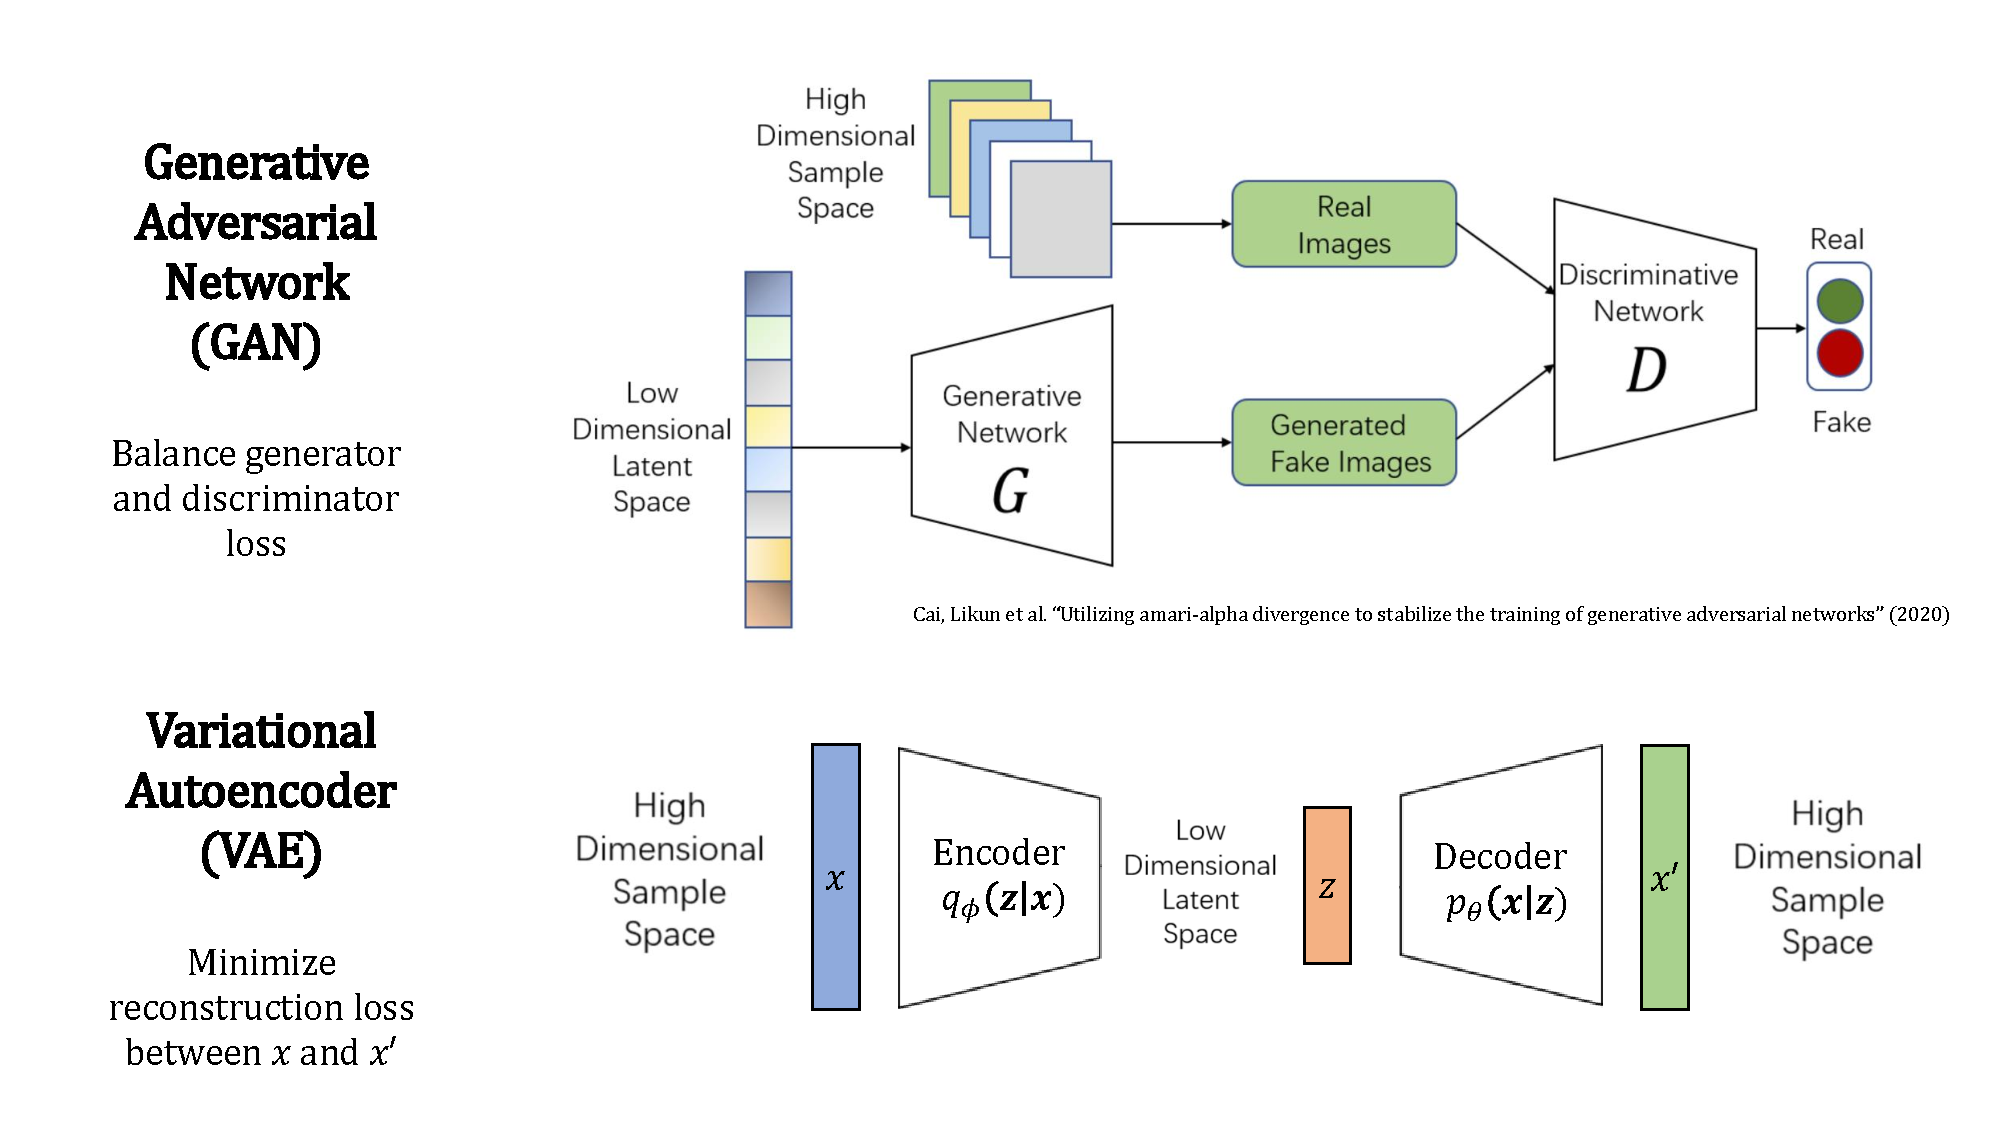
\includegraphics[width=\linewidth]{figs/gan_vae.pdf}
\end{figure*}

Generative Adversarial Networks (GANs) \citep{goodfellow2020generative} estimate generative models through adversarial training with two models: a generator that captures the data distribution and a discriminator which estimates whether a sample came from the generator as opposed to the training data. GANs have been empirically shown to generate higher-quality samples than VAEs \citep{bond2021deep} but require more tuning to synchronize the two models and are prone to problems like vanishing gradients \citep{arjovsky2017towards}, mode collapse, and catastrophic forgetting \citep{thanh2020catastrophic}.

Variational Auto-Encoders (VAEs) \citep{kingma2013auto} are powerful deep generative models that work on unlabeled data and are straightforward to train, as opposed to GANs which require many training tricks for convergence \citep{bond2021deep}. VAEs attempt to map some input $x$ to a latent representation $z$ that can be reconstructed to $x'$, such that the difference between $x$ and $x'$ is minimal. VAEs comprise two jointly learned models: a probabilistic encoder, $q(z|x)$, and a probabilistic decoder, $p(x|z)$.

% \begin{figure*}[ht]
%   \centering
%   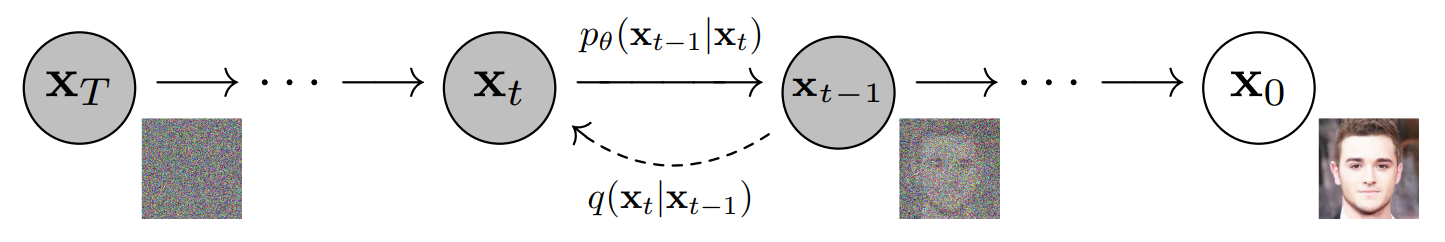
\includegraphics[width=\linewidth]{figs/rel_diffusion.png}
%   \caption{A graphical representation of the forward and reverse diffusion processes in the image domain \citep{ho2020denoising}.}
%   \vspace{0.1in}
%   \label{fig:diffusion}
%   \vspace{-5pt}
% \end{figure*}

% Diffusion probabilistic models (\ie diffusion models) \citep{ho2020denoising} are parameterized Markov chains that learn to reverse an incremental noising process to approximate samples from the target data distribution. Training a diffusion model consists of a forward and backward process. The former incrementally adds Gaussian noise to a data point until at step $T$, the latent representation is approximately Gaussian. The latter learns a parameterization $p(x_{t-1} | x_t)$ to mimic the reverse of the noising function $q(x_t | x_{t-1})$. Diffusion models have been applied in continuous domains to allow for language modeling through diffusion. \citep{li2022diffusion} show that these models are capable of learning complex controls that autoregressive models have failed on. 

\section{Textual Style Transfer}
\label{rel:tst}

Prior work has explored textual style transfer in diverse settings ranging from ``clickbait'' headlines to formalizing text \citep{jin2020hooks, chawla-yang-2020-semi, xu2019clickbait}. While strictly supervised approaches show high fidelity to input samples~\citep{hu2017toward, jhamtani-etal-2017-shakespearizing}, unsupervised and minimally supervised learning are widely applicable since parallel samples are unavailable \citep{shen2017style, yang2018unsupervised}.

Disentanglement, prototype editing, and pseudo-parallel corpus creation are popular approaches for non-parallel data. Prototype editing applies stylistic markers to predefined sentence templates, replacing unwanted parts of the text with text that conforms to a desired attribute \citep{guu2018generating, li-etal-2018-delete}. Disentanglement extracts style independent of the content in a latent space \citep{shen2017style, hu-et-al-controllable}. Pseudo-parallel corpus construction aligns sentences from two mono-style corpora \citep{jin-etal-2019-imat, zhang2018style}. Audience-centric feedback may not conform to the rigid hypotheses of prototype editing and disentanglement. In the case of the former, unconstrained generation allows for freedom in sentence and paragraph-level constructs to define the style \citep{li2020}. For the latter, the separability of content and style is more challenging in specialized domains reliant on domain-specific jargon \citep{woodward2008more} and expressions. Our bootstrapping approach shares some commonalities with pseudo-parallel corpus creation \citep{jin-etal-2019-imat, zhang2018style}, but only utilizes a generic topical corpus to expand the audience-generated ``seed set'' of pairwise judgments. 

Adversarial training has also been used to quantify style \citep{yang-2022-adversarial, John2018}, specifically in disentanglement. \citet{John2018} use auxiliary adversarial and multi-task training objectives to disentangle content from style. For both style and content, they create a multi-task loss to ensure the functionality of the latent representation and an adversarial loss to ensure style does not bleed into content and vice versa. Our approach explicitly decouples the style discrimination and generation tasks for modularity and incremental training purposes, leading to a more robust representation of style.

The evaluation of textual style transfer is generally broken into three parts: fluency, semantic preservation, and strength of the transferred style. Fluency and semantic preservation are well-explored metrics with existing automatic evaluation techniques such as BLEU \citep{Papineni2002bleu}, ROUGE \citep{lin-2004-rouge}, language model perplexity, and BERTScore \citep{zhang2019bertscore}. Most works often use a separately trained stylistic discriminator for automatically evaluating the transferred style strength; however, a robust and reliable classifier requires additional high-quality labeled data, which is problematic in low-resource scenarios. Our approach utilizes the existing pairwise judgments to learn how different linguistic features contribute to the strength of the transferred style.

\section{Controllable Text Generation}
\label{rel:control}

Controllable text generation (CTG) is a fundamental task in natural language generation with a wide variety of applications, such as emotional control in dialogue generation and ensuring that toxic, biased, or discriminatory language is not used in generation. Early literature relied on deep generation models such as variational auto-encoders (VAEs) \citep{guu2018generating, xu2020variational, wang2019topic} and generative adversarial networks (GANs) \citep{scialom2020discriminative} because of the capability of the learned low-dimensional representation to represent linguistic features. \citet{guu2018generating} propose a prototype-then-edit model which generates a sentence by randomly sampling an example from the training set and then applying a randomly sampled edit vector. \citet{scialom2020discriminative} use a GAN-style architecture, training a discriminator to guide the generator toward human-style writing. Recently, \citet{li2022diffusion} utilized diffusion models to denoise a sequence of Gaussian vectors into word vectors while controlling the denoising steps with a gradient-based method, allowing for controllable text generation.

With the recent success of pretrained language models (PLMs), current approaches have generally shifted to a plug-and-play approach to exploit the knowledge from PLMs without significant task-specific retraining. \citet{keskar2019ctrl} attempts to retrain a language model conditioned on control codes ranging from styles and domains (\eg science, politics, horror) to links, questions, and languages. \citet{Dathathri2020Plug} propose using the gradients from simple attribute classifiers (\eg bag of words, single learned layer) during sampling to guide the generation of a PLM. 

\citet{krause2020gedi} guides the generation of a larger PLM using two class-conditional language models, one conditioned on the desired control and one conditioned on the ``anti-control''. Their work resolved the expensive decoding problem from \citet{scialom2020discriminative} and inspired many follow-up works \citep{yang2021fudge, liu-etal-2021-dexperts}. \citet{yang2021fudge} adjusts the output logits of any given PLM with a learned attribute predictor that predicts whether an attribute will be true in the future, as opposed to existing work which judges based on the present. 

Many approaches have also attempted to control generations during decoding. \citet{liu-etal-2021-dexperts} steers the output distribution of a PLM with an ensemble of ``expert'' and ``anti-expert'' LMs by obtaining the outputs of all LMs at timestep $t$ based on prompt $x_{<t}$, obtaining $z_t$ (from the PLM), $z_t^+$ (from the ``expert''), and $z_t^-$ (from the ``anti-expert''). The resulting distribution (\ie product-of-experts ensemble) is:

\begin{equation}
    \tilde{P}(X_t | x_{<t}) = \text{softmax}(z_t + \alpha (z_t^+ - z_t^-))
\end{equation}

where $\alpha$ is a hyperparameter that controls the amount of change to $z_t$. \citet{kumar2021controlled} formulates decoding as an optimization problem with multiple differentiable constraints: a primary negative log-likelihood constraint (for fluency) and multiple secondary constraints for desired attributes.

To summarize, existing approaches only empirically evaluate three types of control conditions: semantic (\eg emotion, topics), structural (\eg syntax tree, parts-of-speech), and lexical controls (\eg keyword/phrase inclusion) \citep{Zhang2022ASO}. Furthermore, while some studies claim to support multiple controls during text generation, there has been little evidence for any such technique. Our work addresses the former by exhibiting control over speed \citep{toubia-2021}, a linguistic feature that does not cleanly fall into the three control conditions. We leave it to future work to text and explore methods to condition text on multiple controls effectively.

In the next chapter, we introduce the task of \textit{style infusion} and propose a novel approach to infuse audience-centric styles into pretrained language generation models.






\ctparttext{
    \lipsum[2]
}
\chapter{Style Infusion as a Control}\label{chp:style_infusion}
In this chapter, we introduce a method to infuse audience-centric styles into pretrained language generation models. Specifically, we bootstrap an initial style analysis model to discriminate the positive and negative samples from audience feedback. Our model then selects additional samples from a generic topical sentence collection to expand the seed set of audience judgments. By separating style analysis and text generation models, we create an adversarial setup to infuse the audience's stylistic feedback in any generative LM. We weight the noisy reward from the style analysis model (discriminator) with a reconstruction loss to balance style adoption and fluency. We test our approach on two audience-centric styles, persuasion, and memorability, including empirical and qualitative evidence to show that our infusion approach generates compelling stylized examples with generic text prompts.\footnote{This work has led to the following publication: Samraj Moorjani, Adit Krishnan, Hari Sundaram, Ewa Maslowska, and Aravind Sankar. ``Audience-Centric Natural Language Generation via Style Infusion.'' \textit{Findings of the Association for Computational Linguistics: EMNLP 2022} \citep{moorjani-etal-2022-audience}.}

In summary, our abbreviated contributions are as follows: 
\begin{enumerate}
    \item \textbf{Audience-centric Style Infusion}: We introduce the task of style infusion to tether the definition of style to the target audience. By utilizing explicit audience feedback via pairwise comparisons, we promote a more human- and audience-centric approach to text styling.
    
    \item \textbf{Decoupling Style}: We propose an automatically weighted loss to decouple the training objectives of the style discriminator and text generation model, leading to a more robust representation of style than in fused settings.

    \item \textbf{Automatic Style Evaluation}: We present an automatic evaluation metric for quantifying the transfer of audience-centric styles by computing the correlations of linguistic features with a given style. We then evaluate our model's generations based on their agreements with the audience-derived correlations. 
\end{enumerate}
% Persuasiveness Scorer Section
\section{Discriminative Language Model}
\label{sec_discriminator}

In this section, we train a BERT-based style discriminator on pairwise audience judgements to provide feedback to our generator. In~\Cref{subsec:discrim_arch}, we describe the architecture and training details along with the pairwise feedback datasets in~\Cref{subsection:pairwise_datasets}. Then in~\Cref{subsec:discrim_obse}, we present the results of the style discriminator and in~\Cref{subsec:siamesebert}, we describe an alternate approach with a Siamese BERT discriminator.

\subsection{Model Architecture and Training}
\label{subsec:discrim_arch}

Our style discriminator (style analysis module) adds a fully connected (FC) layer with dropout to pre-trained BERT~\citep{devlin-etal-2019-bert}. We use the 'bert-base-uncased' model from the Huggingface Transformers library \citep{wolf2019} (12-layers, 768 dimension). We concatenate with a '$\langle$SEP$\rangle$' token and jointly tokenize the compared pair of sentences. The FC layer generates a single output ($\mathbb{R}^{768} \rightarrow \mathbb{R}$). We threshold the sigmoid of the output at 0.5 to decide the preferred sentence. We train all layers (including BERT) on the pairwise audience feedback (batch size 32, 5 epochs, $\eta=0.0001$, dropout~$=0.2$). 
% We also train a Siamese BERT architecture \citep{reimers2019} with the same settings but find it to underperform BERT (results in~\Cref{subsec:siamesebert}).

\subsection{Pairwise Feedback Datasets}
\label{subsection:pairwise_datasets}
% Quantifying a specific style of an argument is a challenging task for humans, but labeling which of two arguments is more likely to contain that style is much easier. 
We select one pairwise feedback dataset for both the persuasiveness and memorability tasks to evaluate our approach. The UKPConvArg1 corpus~\citep{habernal-gurevych-2016-argument} presents pairs of arguments where human annotators select the more persuasive argument. The authors generate 16,000 argument pairs over 16 distinct, non-overlapping topics. Both arguments in a pair belong to the same topic and argue for the same stance (\ie parallel pairwise feedback). For memorability, we leverage the Cornell Movie-Quotes Corpus~\citep{danescu-niculescu-mizil-etal-2012-hello}, containing 2,200 paired movie quotes with crowd-sourced memorability annotations. 

\subsection{Observations and Validation}
\label{subsec:discrim_obse}
Our discriminator achieves 89\% accuracy over 5-fold cross-validation for the persuasiveness task. We further validate for overfitting by holding out two topics from the test set and training on the remaining topics, ensuring the discriminator has no exposure to these held-out topics during training. After training from scratch, the discriminator still achieves 87\% accuracy on the held-out topics. On the Cornell Movie-Quotes corpus, the discriminator achieves  80\% accuracy. We repeat the held-out topic test to validate the classification performance for the memorability task.

In summary, these tests validate the ability of our style discriminator to learn audience style preferences with small volumes of pairwise feedback. In \Cref{sec_generator}, we describe our approach to infuse the style discriminator feedback into a generative language model.

\subsection{Siamese BERT Discriminator}
\label{subsec:siamesebert}

To further validate our results, we tried another architecture, similar to Siamese BERT \citep{reimers2019}, where we tokenized the texts individually and passed them through their own BERT layers, producing two embeddings, $e_1$ and $e_2$. We concatenated the two outputs along with the distance between the two as follows:
\begin{equation}
    [e_1 ; e_2 ; |e_2 - e_1|]
\end{equation}
We passed this new vector of $\mathbb{R}^{3 \times h}$, where $h$ is the hidden dimension of BERT, through a fully connected classification layer.

While the original discriminator achieves approximately 89\% accuracy on the random test set, the Siamese BERT model achieves a smaller, but still significant, 83\% accuracy. On the Cornell Movie-Quotes corpus, with the same hyperparameters, the original discriminator achieves 80\% accuracy and a 77\% accuracy with the Siamese BERT architecture. We choose to use the simpler discriminator architecture because it seems to capture style better than the Siamese BERT architecture. 
\section{Style-Aware Language Generation}
\label{sec_generator}

\begin{figure*}[ht]
  \centering
  \caption{Training diagram that shows how the loss is calculated as a weighted sum of the discriminator ($L_{D}$) and reconstruction ($L_{R}$) loss. $\alpha_S$ is decided by the discriminator as a form of contrastive learning.}
  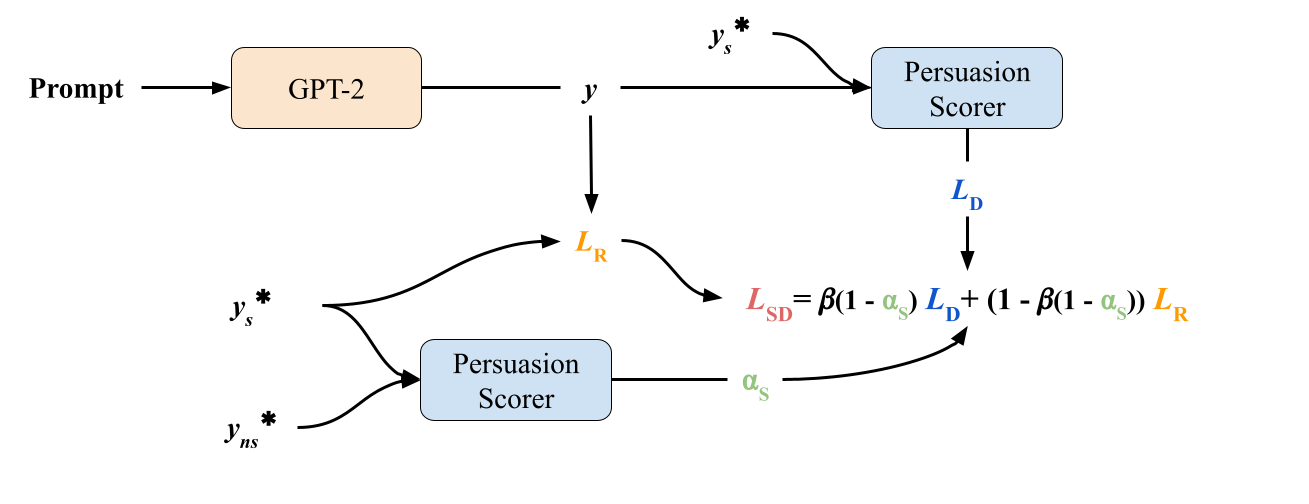
\includegraphics[width=0.9\linewidth]{figs/Architecture.png}
  \label{fig:architecture}
  \vspace{-5pt}
\end{figure*}

In this section, we infuse the stylistic preferences learned by our style discriminator in \Cref{sec_discriminator} into a GPT-2 model~\citep{radford2019language} pretrained on the causal language modeling (CLM) objective~\footnote{https://huggingface.co/gpt2}. The model takes in a textual prompt and generates text, $y$, that we want to infuse with the audience preferred style. For the persuasiveness task, the UKPConvArg1 dataset provides prompts for each argument pair. For the memorability task, we use the previous sentence as the prompt.

During training, we feed the prompt and feedback pair to GPT-2 - the more preferred (styled) sample, $y^*_s$, and the corresponding less-preferred (non-styled) sample, $y^*_{ns}$. We use an adversarial training paradigm to enable the generator to learn from the discriminator, illustrated in~\Cref{fig:architecture}. 

In~\Cref{subsec:si_training}, we introduce the custom loss function used for training. Then in~\Cref{subsec:si_dataset}, we discuss our augmentation approach for pairwise style data. Lastly, in~\Cref{subsec:si_gpt}, we describe GPT-2 and its benefits over other generation architectures.

\subsection{Training}
\label{subsec:si_training}

We utilize two losses during training: a reconstruction loss, $L_R$, and a discriminator loss, $L_D$. The reconstruction loss maximizes the log probability of the styled argument, $y_s^*$.

\begin{equation}
    L_{R} = -\frac{1}{N} \sum_{i=1}^{N} \log p(y_s^{*(i)})
\end{equation}

The reconstruction loss teaches the model to mimic the gold-standard samples. The discriminator loss maximizes the score of the discriminator, $\mathcal{D}$, and is formulated as:

\begin{equation}
    L_{D} = \mathcal{D}(y_s^*, y) - \frac{1}{N} \sum_{i=1}^{N} \hat{R}_i \log p(y^{(i)})
\end{equation}

where $y^{(i)}$ is the $i$-th token of the generated sentence $y$, and $\hat{R}_i$ is a baseline reward meant to reduce the noise from the discriminator. The baseline reward is meant to reduce the noise from the reward given by our discriminator \citep{ranzato2015sequence}. The baseline reward, $\hat{R}_i$, is calculated using a linear layer, with the input being the hidden states of our generator at timestep $i$. The intuition is that the linear layer approximates the value of the reward for a certain timestep and in practice, reduces the variance from the reward. We train the linear layer with the following loss:

\begin{equation}
    L_{BR} = \frac{1}{N} \sum_{i=1}^{N} |\mathcal{D}(y_s^*, y) - \hat{R}_i|^2
\end{equation}

where $\mathcal{D}(y_s^*, y)$ is the output of the discriminator when fed a gold argument and the generated argument (i.e. the reward). 

We find that too strong of a discriminator loss negatively impacts fluency. Thus, we introduce a regularization constant, $\beta$, to ensure that the discriminator loss remains only a fraction of the loss. The two losses are weighted together to create the final loss as follows:

\begin{equation}
    L_{SD} = C \cdot L_{D} + (1-C) \cdot L_{R}
\end{equation}

where $C = \beta (1-\alpha_{S})$ and $\alpha_{S} = \mathcal{D}(y_s^*, y_{ns}^*)$. Note that $y_{ns}^*$ is the non-styled training argument. 

Instead of making the weighted ratio between the two losses constant, we make them sample dependent. The intuition is that when $\alpha_{S}$ is high (e.g. the sample is persuasive), we can just use the reconstruction loss to replicate the gold standard which will directly reflect the style. However, when $\alpha_{S}$ is low (i.e. we have a weak sample), we instead switch to learning the trends from the discriminator. This loss is referred to as the sample-dependent discriminator (SD) loss. We also compare the discriminator loss with a simpler supervised loss defined as $L_{S} = \frac{1}{N} \sum_{i=1}^{N} \mathcal{D}(y_s^*, y^{(1..i)})$.

% \begin{equation}
%     L_{S} = \frac{1}{N} \sum_{i=1}^{N} \mathcal{D}(y_s^*, y^{(1..i)})
% \end{equation}

\subsection{Dataset Augmentation Approach}
\label{subsec:si_dataset}

The UKPConv1 and Cornell Movie Quotes corpora we presented in~\Cref{subsection:pairwise_datasets} provide approximately 16,000 and 2,200 unique pairs for stylistic feedback; not nearly enough to train a large language model. To increase our model's breadth of knowledge, we generate additional pairwise feedback with the CNN/Daily Mail dataset \citep{see-etal-2017-get}, containing over 300,000 unique news articles. 

First, we generate the Universal Sentence Embeddings~\citep{cer-2018} of all unique sentences in our style corpora (UKPConv1, Cornell) and external corpora (CNN/Daily Mail). For each candidate sentence in the external dataset, $s_i$, we find the top-k similar sentences ($y_1 ... y_k$) in the style corpus to be augmented. We then perform pairwise comparisons $\lor_{j} \mathcal{D}(s_i, y_j) > 0.5, j \in \{1, ..., k\}$ where if the discriminator prefers the candidate external sentence ($s_i$) over \textit{any one} of the similar sentences ($y_1 ... y_k$) from the style corpus, we include the pair. Through this bootstrapped augmentation method, we ensure we have sentences that are relatively more ``styled'', as defined by our discriminator, and similar to those in our existing corpus. 

\subsection{Style-Aware Generation with GPT-2}
\label{subsec:si_gpt}

The OpenAI GPT-2 \citep{radford2019language} model is a large transformer-based language model pretrained on nearly 8 million web pages, allowing generalization to many domains and tasks. This is closer to the unconstrained scenarios that we wish to target with our style-infusion task. Alternate generators such as pointer-generators rely on copying~\citep{xu2019clickbait}, thus introducing more limitations in the extent of style infusion. The ability to extensively pretrain transformer-based models makes them more widely applicable for syle infusion~\citep{gururangan2020pretraining}.

In this section, we introduced the adversarial training mechanism for the style-aware language generator and the bootstrapped data augmentation method used to produce robust generations. Next, we will introduce the baselines, evaluation metrics, and training settings.

% We found that the pre-trained GPT-2 provided by Huggingface ran into many issues with fluency and degeneration. Instead, we utilize GPT-2 fine-tuned on news data to provide an initial breadth of knowledge and diversity in generations. 
\section{Experiments}
\label{sec:si_experiments}

In this section, we describe the baseline approaches (\S\ref{subsec:si_baseline}) along with the experimental settings used (\S\ref{subsec:si_exp}). In~\Cref{sec:style_strength}, we present our novel automatic evaluation method for the strength of the infused style. Lastly, in~\Cref{subsec:si_similarity}, we discuss the automatic lexical and semantic similarity metrics used to evaluate our approach.

\subsection{Baselines}
\label{subsec:si_baseline}

We compare our architecture against a few strong baselines:

\textit{\textbf{Pretrained GPT-2}} \citep{radford2019language} We use this pre-trained model as a representation of average text, allowing us to show shifts in style that occur due to training.

\textit{\textbf{Fine-tuning}} We fine-tune the pre-trained GPT-2 model using the reconstruction objective on the style-specific corpus only (e.g. UKPConv1).

\textit{\textbf{Fine-tuning + Data Augmentation}}  We fine-tune the pre-trained GPT-2 model using the reconstruction objective on the augmented data.

\textit{\textbf{TitleStylist}} \citep{jin2020hooks} We adapt the stylistic headline generation framework to generate stylistic text based on a prompt. \citet{jin2020hooks} utilize a Denoising Autoencoder with parameter sharing to disentangle style from content to control the style with a set of parameters.  

\subsection{Experimental Settings}
\label{subsec:si_exp}
For all GPT-2 based models, we use a base GPT-2 model from Huggingface \citep{wolf2019} (1024 dimensions, Adam optimizer, $\eta = 5e-5$). Because of the length of our text and size of our models, we utilize DeepSpeed \citep{rasley-2020-deepspeed} to distribute training over two 32GB V100s, and we train with FP16 mixed precision. We experiment with the loss parameters of $C$ and $\beta$ and discuss our findings in~\cref{section:discussion}. 
% , using $0.1, 0.5, 0.8$, and $1.0$. We also experiment with hard-coded values of the coefficients in the weighted loss. For example, we tried a setting with 90\% of the weight going to $L_{R}$ and 10\% going to $L_{S}$. 

% \section{Evaluation Metrics} 
% In this section, we detail the evaluation metrics used to ensure our model was able to effectively transfer style while preserving content and fluency.

\subsection{Infused Style Strength}
\label{sec:style_strength}

We take a deeper look into the annotator labels in the UKPConvArg1 dataset and we find that some linguistic features play a significant role in the persuasiveness of text. We create a hierarchical Bayesian model to find the correlation between a set of collected linguistic features and the desired style. We first take the unique sentences from a dataset and compute a set of linguistic features over them. A full list of features can be found in~\Cref{apx:lfc}.

We define the hierarchical Bayesian model as a binomial distribution around $p$. Note that text A always demonstrates the style more strongly than text B or equally to text B. We calculate $p$ as follows:

\begin{equation}
    logit_p = \bar{p} + (\alpha[A_{id}] - \beta[B_{id}]) + \gamma[t] * (A_{ft} - B_{ft})
\end{equation}

where $\bar{p}$ is the intercept, $\alpha$ and $\beta$ are meant to capture any existing bias towards either text and $\gamma$ measures the correlation between the linguistic feature and the style for a specific topic $t$. We construct $\alpha$ and $\beta$ for all texts, hence why we index them with $A_{id}$ and $B_{id}$, respectively. Similarly, we construct $\gamma$ for each topic. $A_{ft}$ and $B_{ft}$ are the features of text A and B, respectively. $\alpha$, $\beta$, and $\gamma$ are all constructed similarly. Let's take $\alpha$ as an example:

\begin{equation}
    \alpha = \bar{\alpha} + \alpha_{v} \alpha_{\sigma}
\end{equation}

where $\bar{\alpha} \sim \mathcal{N}(0, 0.25)$ and $\alpha_{\sigma}$ is drawn from an exponential distribution with $\lambda = 1$. We construct a separate $\alpha_{v}$ for each unique $A_{id}$ where each $\alpha_{v} \sim \mathcal{N}(0, 1.0)$. These values are chosen because they help the MCMC sampling converge. $\beta$ and $\gamma$ follow the same construction except with different shapes for $\beta_{v}$ and $\gamma_{v}$. 

For each linguistic feature-topic pair, we infer the correlation between the feature and the text that demonstrates the style by running a Markov Chain Monte-Carlo (MCMC) process using the No-U-Turn Sampler (NUTS). During the training of the hierarchical Bayesian model, we use 1000 warmup steps and generate an additional 1000 samples. Note that the results we show are in the logit scale, meaning even a change of $\mp 1$ has a big effect on the probability (about a 23\% difference in odds of winning).  

The models then generate text based on the prompts in a held-out test set and we calculate the features of the generations. We run a t-test to determine if the difference in features between a pretrained GPT-2 and one of our models is statistically significant. This evaluation shows how our trained model learns to use these linguistic features to construct more stylized arguments.

\subsection{Semantic and Lexical Similarity Metrics}
\label{subsec:si_similarity}

In addition, we use \textit{pyrouge} library to collect the ROUGE \citep{lin-2004-rouge} score, a commonly used metric that measures the N-gram overlap between the training and generated arguments. While these scores will not tell us how persuasive our generations are, they will ensure that the generations remain on topic.

Lastly, we compute the BERTScore \citep{zhang2019bertscore}, another automatic evaluation metric that computes token similarity using contextual embeddings. The BERTScore represents the semantic similarity of the generations to the test set which will ensure generations are relevant, but not necessarily persuasive.
\section{Results on Persuasiveness}
\label{sec:pers_results}

In this section, we analyze our results by showing a significant usage of linguistic features that resemble persuasive text (\S\ref{subsec:si_pers_corr}), showing generated text (\S\ref{subsec:si_pers_sample}), and with standard metrics (\S\ref{subsec:si_pers_auto}).  

\subsection{Linguistic Feature Correlations}
\label{subsec:si_pers_corr}

\Cref{fig:feature_correlations} shows the correlations between linguistic features and convincingness in the UKPConvArg1 corpus. The model details are in~\Cref{apx:lfc}.
% Persuasiveness Feature Correlations
\begin{figure}[h]
  \centering
  \caption{The correlations between linguistic features and convincingness in the UKPConvArg1 corpus. The lower x-axis is in the logit scale, and the percentage difference in odds of winning is on the upper x-axis. The figure is read as: if the feature for argument A is one standard deviation greater than the feature for argument B, the odds of A winning shift by the respective percent value. Notice that the correlations show a strong positive correlation with readability (\eg the Flesh score is positive while length and average syllables are negative). }
  \label{fig:feature_correlations}
  \scalebox{1.0}{
  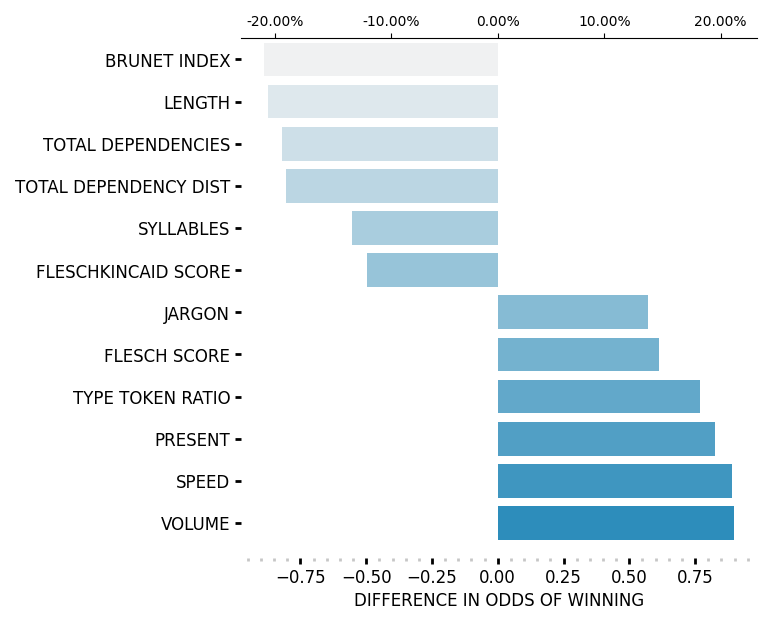
\includegraphics[width=\linewidth]{figs/16k_corr.png}
  }
\end{figure}

We find a strong positive correlation between readability and winning arguments. This is reflected by both readability scores (\eg SMOG, Flesch-Kincaid, etc.) and correlation with smaller words, fewer total dependencies, and a smaller overall total dependency distance. We notice a positive correlation with speed and volume. \citet{toubia-2021} define speed as the total distance covered by a text's word embeddings, normalized by the length of the text. Volume represents the amount of material covered by the text, calculated by estimating the volume enclosed by the word embeddings \citep{toubia-2021}. We also find a negative correlation with passive voice and a positive correlation with misspelled words (not shown for brevity).

We run a significance test to see how well our models learned the style (see~\Cref{apx:featureagreement}). Most models consistently learn pronounced trends (\ie Brunet index, length, speed, and volume). The augmented data likely led to this change because fine-tuning on the augmented set displays the same trends. In cases like total dependencies (TD) and the ratio of present tense verbs, models trained with the sample-dependent discriminator (SD) loss are significantly better at learning the trend, despite the data not actively showing the trend (or completely opposing it). In the case of Flesch score, models trained with SD loss can nullify the trend which occurs in the incorrect direction. This displays that models trained with the SD loss are substantially better at learning from the dataset than the baselines and models trained with the sample-dependent supervised (SS) loss. One example of failure is the ratio of jargon, likely because the model could not generate out of vocabulary words, but this is a limitation of how we define jargon.

% We also show the results of Table~\Cref{tab:feature-evaluation} in the context of the full feature set in the Appendix by computing an agreement score. 


\subsection{Sample Generations}
\label{subsec:si_pers_sample}



% Persuasiveness Sample Generations

  \begin{table}[htb]
  \small
  \centering
  \caption{The baseline models and our model (GPT2 with the SD loss and $\beta=0.5$ on the augmented data). The models are fed the input ``Plastic bottles are bad because'' and ``Gaming is good for child development because'', generating up to 100 tokens using beam search.}
  \label{tab:example_persuasive} 
  \begin{tabularx}{\linewidth}{@{}>{\raggedright\arraybackslash}X@{}}
   \toprule[1.5pt]
  \textsc{Model} \& \textsc{Generated Text}\\
  \midrule[0.75pt]
  \textsc{Example 1:}\\
  \textbf{GPT2}:  Plastic water bottles are bad because they are not recyclable," he said. "They are not good for the environment, they are not recyclable."  \\
  \textbf{GPT2-Aug}: Plastic water bottles are bad because it causes pollution. Also water bottles also cost more than regular water. \\
  \textbf{TStylist}: Plastic water bottles are bad because plastic water bottles are bad for our environment.\\
  \textbf{Ours (SD-0.5)}: Plastic water bottles are bad because they are not recycled and end up in landfills which lead to pollution of our environment. Plastic requires up to 47 million gallons of oil per year to produce.  \\
  \addlinespace[0.5em]
  \textsc{Example 2:}\\
  \textbf{GPT2}: Gaming is good for child development because it teaches them how to use a computer. It's good for the economy, it's good for the environment, it's good for the children, it's ...  \\
  \textbf{GPT2-Aug}: Gaming is good for child development because it allows the child to grow and develop. I believe eSports (LoL) should be a spectator sport and not a major part of the sports calendar.   \\
  \textbf{TStylist}: Gaming is good for child development because gaming is good for your child.\\
  \textbf{Ours (SD-0.5)}: Gaming is good for child development because it allows children to grow up in a world where they are exposed to a wide variety of ideas and experiences.   \\
  \bottomrule[1.5pt]\\
  \end{tabularx}
  \vspace{-10px}
  \end{table}


\Cref{tab:example_persuasive} shows the generations of three baselines and our best-performing method. We find that for both prompts, the generations of models trained with the sample-dependent discriminator (SD) loss generally have the highest values of speed, volume, and lexical diversity. For the second prompt, the speed and volume of our generation are larger than that of GPT2 and TStylist, but slightly smaller than that of GPT2 fine-tuned on the augmented data. Intuitively, this makes sense because the GPT-Aug generation covers much more information in the same time frame; however, this information isn't relevant to the argument, making our generation much more sensible. The baselines often suffer from neural degeneration, but the model trained with the SD loss does not face this issue. Since length had a strong negative correlation with persuasiveness, the model likely implicitly learned from the discriminator to handle this kind of neural degeneration. However, it is still an issue in some cases with out-of-domain samples.






% Persuasiveness ROUGE
  \begin{table}[htb]
  \centering
  \small
  \caption{ROUGE-\{1,2, L\} scores and BERT scores (F1) for all models. Baseline models: GPT2, GPT-2 fine-tuned on UKPConvArg1, GPT-2 with augmented data, TitleStylist \citep{jin2020hooks}. Our models are trained on augmented data and a sample-dependent discriminator (SD) or sample-dependent supervised (SS) loss with parameter $\beta$. The baseline ROUGE score increases due to data augmentation; the relevance of our models' generations is largely insensitive to loss type and parameter value.}
  \label{tab:automatic-evaluation}
  \scalebox{1.0}{
  \begin{tabularx}{0.9\linewidth}{@{}>{\raggedright\arraybackslash}Xcccc@{}}
   \toprule[1.5pt]
  \textsc{Model} & \textsc{RG-1}            & \textsc{RG-2}           & \textsc{RG-L}        &\textsc{B-F1} \\     
  \midrule[0.75pt]
  GPT2     & 0.1856          & 0.0968          & 0.1769         & 89.28          \\
  GPT2-UKP & 0.2474          & 0.1061          & 0.1989         & 87.21         \\
  GPT2-Aug & 0.2987          & 0.1845          & 0.2774         & 86.90          \\ 
  TStylist & 0.2578          & 0.1569          & 0.2391         & 84.70          \\ 
  \midrule[0.75pt]
  % \addlinespace[0.5em]
  SS-0.1   & 0.2925          & 0.1802          & 0.2717         & 88.95          \\
  SS-1.0   & 0.2862          & 0.1774          & 0.2634         & 89.18          \\
  SD-0.1  & 0.3036          & 0.1903          & 0.2802          & 88.75         \\
  SD-0.5  &    \textbf{0.3168} & \textbf{0.2296} & \textbf{0.3065 } & \textbf{89.56}       \\
  SD-0.8  & 0.2872          & 0.1957          & 0.2733          & 89.12         \\
  SD-1.0  & 0.2929          & 0.2224          & 0.2848          & 89.05         \\ 
  \bottomrule[1.5pt]\\
  \end{tabularx}
  }
  \vspace{-25pt}
  \end{table}
%   \begin{table}[htb]
  
%   \centering
%   \small
%   \caption{ROUGE-\{1,2, L\} scores for all models. Baseline models: GPT2, GPT-2 fine-tuned on UKPConvArg1, GPT-2 with augmented data, TitleStylist \citep{jin2020hooks}. Our models are trained on augmented data, and a sample-dependent discriminator (SD) or sample-dependent supervised (SS) loss with parameter $\beta$. The baseline ROUGE score increases due to data augmentation; the relevance of our models' generations is largely insensitive to loss type and parameter value.}
%   \label{tab:automatic-evaluation}
%   \scalebox{1.0}{
%   \begin{tabularx}{0.85\linewidth}{@{}>{\raggedright\arraybackslash}Xccc@{}}
%   \toprule[1.5pt]
%   \textsc{Model} & \textsc{RG-1}            & \textsc{RG-2}           & \textsc{RG-L} \\     
%   \midrule[0.75pt]
%   GPT2     & 0.1856          & 0.0968          & 0.1769                    \\
%   GPT2-UKP & 0.2474          & 0.1061          & 0.1989                   \\
%   GPT2-Aug & 0.2987          & 0.1845          & 0.2774                    \\ 
%   TStylist & 0.2578          & 0.1569          & 0.2391                    \\ 
%   \midrule[0.75pt]
%   % \addlinespace[0.5em]
%   SS-0.1   & 0.2925          & 0.1802          & 0.2717                    \\
%   SS-1.0   & 0.2862          & 0.1774          & 0.2634                    \\
%   SD-0.1  & 0.3036          & 0.1903          & 0.2802                    \\
%   SD-0.5  &    \textbf{0.3168} & \textbf{0.2296} & \textbf{0.3065 }         \\
%   SD-0.8  & 0.2872          & 0.1957          & 0.2733                    \\
%   SD-1.0  & 0.2929          & 0.2224          & 0.2848                    \\ 
%   \bottomrule[1.5pt]\\
%   \end{tabularx}
%   }
%   \vspace{-25pt}
%   \end{table}


\subsection{Automatic Metrics}
\label{subsec:si_pers_auto}
We compare the ROUGE scores of our experimental models in ~\Cref{tab:automatic-evaluation}, ensuring that the topics in the test set are not discussed anywhere in the UKPConvArg1 or augmented datasets. The data augmentation leads to a sharp increase in the ROUGE scores of the generations, showing that it is essential for robust and relevant generations. The results are relatively insensitive to variation in $\beta$ parameter that controls the tradeoff between reconstruction loss ($L_R)$ and discriminator loss ($L_R$). These scores show that our models generate relevant, but not necessarily persuasive, text. We find similar insights from the BERTScore; although the augmentation has a slight negative impact on the score, the difference is negligible. 

\section{Results on Memorability}
\label{sec:mem_results}

In this section, we focus on memorability and show that our model can generate more robust, relevant, and memorable text than the baselines. In~\Cref{subsec:si_mem_corr}, we find linguistic features that are strongly correlated with memorability. Then in~\Cref{subsec:si_mem_sample}, we show samples of generated text and lastly, in~\Cref{subsec:si_mem_auto}, we present the results on our automatic metrics.

\subsection{Linguistic Feature Correlations}
\label{subsec:si_mem_corr}
% Memorability Feature Correlations
% \begin{wrapfigure}{r}{0.5\textwidth}
\begin{figure}[t]

  \centering
  \caption{The correlations between linguistic features and persuasiveness in the Cornell Movie-Quotes Corpus. The lower x-axis is in the logit scale, and the percentage difference in odds of winning is on the upper x-axis. Notice that the correlations show a negative correlation with long and winding text (\ie circuitousness \citep{toubia-2021}). }
  \label{fig:mem_feature_correlations}
  \scalebox{1.0}{
    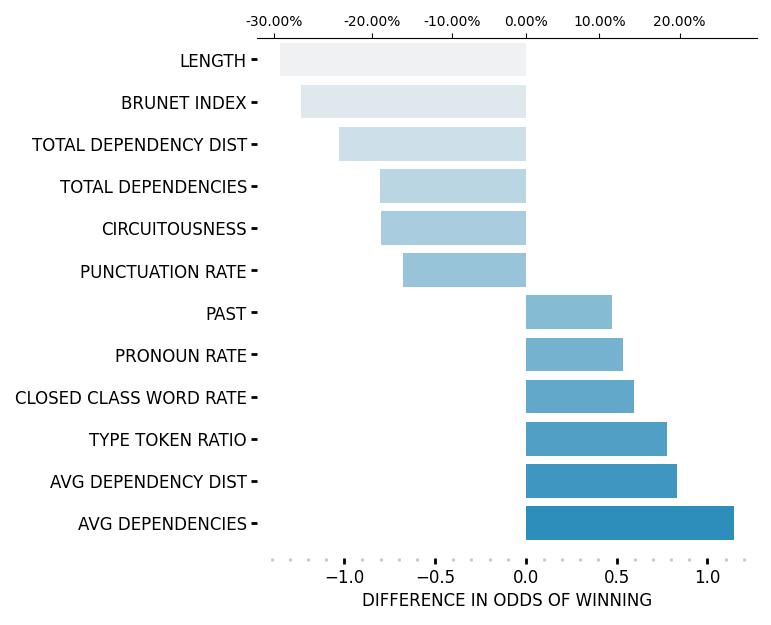
\includegraphics[width=\linewidth]{figs/imdb_corr.png}
  }
\end{figure}
% \end{wrapfigure}

We train a Bayesian hierarchical model for the Cornell Movie Quotes corpus, which produces the correlations shown in~\Cref{fig:mem_feature_correlations}. We find a strong negative correlation with long, winding text, shown by the trends in total dependencies, total dependency distance, length, and circuitousness. A higher circuitousness implies that a less direct route was taken to convey information \citep{toubia-2021}. Circuitousness is detrimental to memorability as winding text tends to be harder to remember. The negative correlation with the punctuation rate and positive correlation with the average dependencies show that more memorable text tends to have a few sentences, independent of the length of sentences. Lastly, there is a strong emphasis on uncommon vocabulary with a negative correlation with the Brunet index and a positive correlation with token type ratio. This is supported by findings from \citep{danescu-niculescu-mizil-etal-2012-hello} who find that memorable quotes are built upon less common word choices. 

We run the significance test on a held-out test set to see how well our models learned to generate memorable text. In some cases in~\Cref{tab:mem-feature-evaluation}, models trained with the sample-dependent discriminator (SD) loss have similar performance as the fine-tuned models, indicating that some relevant features are learned solely from fine-tuning. However, many other incorrect trends are corrected with training using the SD loss. The only feature that does not improve is the pronoun rate, likely because of shorter sentences with more emphasis on uncommon word choices. 

\subsection{Sample Generations}
\label{subsec:si_mem_sample}

We look at a few examples of generations to see how training influenced the model's generations in~\Cref{tab:example_the_more}. There is a visible decrease in the number of sentences, overall length, and circuitousness in both the GPT2-Aug and SD-0.5 models. This reflects the trends shown in~\Cref{tab:mem-feature-evaluation}, but we can see that the model trained with the SD loss generates sentences that are more sophisticated than the fine-tuned GPT2 model's. TitleStylist generates sentences that are identical to our generation feature-wise but are not as sophisticated as our generations.

% Memorability Sample Generations
% \mbox{}
  \begin{table}[htb]
%   \vspace{-15pt}
  \small
  \centering
  
  \begin{tabularx}{\linewidth}{@{}>{\raggedright\arraybackslash}X@{}}
  \caption{Generations of GPT2, GPT2 fine-tuned on augmented data, and GPT2 with the SD loss ($\beta=0.5$) on the augmented data. The models are fed in the inputs ``The more you'' and ``When solving problems, dig''.}
  \label{tab:example_the_more}
   \toprule[1.5pt]
  \textsc{Model} \& \textsc{Generated Text}\\
  \midrule[0.75pt]
  \textsc{Example 1:}\\
  \textbf{GPT2}:  The more you know about it, the more likely you are to believe that it is true. If you don't believe that it is true, you're not alone. If you don't believe that it is true, you're not alone... \\
  \textbf{GPT2-Aug}: The more you smoke, the more you will smoke  \\
  \textbf{TStylist}: The more you need to know. \\
  \textbf{Ours (SD-0.5)}: The more you learn, the more you see.  \\
  \addlinespace[0.5em]
  \textsc{Example 2:}\\
  \textbf{GPT2}: When solving problems, dig a hole in the ground and dig a hole in the ground and dig a hole in the ground and dig a hole in the ground and ...    \\
  \textbf{GPT2-Aug}: When solving problems, dig your heels in and try to find a solution, even if you don't have the answers, and even if you don't know the answers. \\
  \textbf{TStylist}: When solving problems, dig better and better.\\
  \textbf{Ours (SD-0.5)}: When solving problems, dig deeper than a grave.   \\
  \bottomrule[1.5pt]

  \end{tabularx}
  \end{table}
  
\vspace{-0.25in}

 \subsection{Automatic Metrics}
 \label{subsec:si_mem_auto}
Similar to persuasiveness,~\Cref{tab:mem-automatic-evaluation} shows that the ROUGE scores increase mainly due to data augmentation. Once again, these results demonstrate that the augmented data leads to more relevant generations, increasing the breadth of knowledge transferred to the model. The same trends generally hold for the BERTScore, which shows that the generations remain semantically relevant.

% Memorability ROUGE

\begin{table}[t]
  \centering
  \small
  \caption{ROUGE-\{1,2, L\} scores and BERT scores (F1) for all models. Baseline models: GPT2, GPT-2 fine-tuned on UKPConvArg1, GPT-2 with augmented data, TitleStylist \citep{jin2020hooks}. Our models are trained on augmented data, and a sample-dependent discriminator (SD) or sample-dependent supervised (SS) loss with parameter $\beta$. The baseline ROUGE score increases due to data augmentation; again, the relevance of generations is largely independent of loss type and parameter value.}
  \label{tab:mem-automatic-evaluation}
  \begin{tabularx}{0.9\linewidth}{@{}>{\raggedright\arraybackslash}Xcccc@{}}
   \toprule[1.5pt]
  \textsc{Model} & \textsc{RG-1}            & \textsc{RG-2}           & \textsc{RG-L}    & \textsc{B-F1} \\     
  \midrule[0.75pt]
GPT2      & 0.1503          & 0.0853          & 0.1461          & 81.12          \\
GPT2-IMDB & 0.1579          & 0.0853          & 0.1510          & \textbf{88.87}          \\
GPT2-Aug  & 0.2737          & 0.1703          & 0.2685          & 87.24          \\
TStylist  & 0.2542          & 0.1617          & 0.2439          & 85.99          \\
  \midrule[0.75pt]
  % \addlinespace[0.5em]
  SS-0.1  & 0.2746          & \textbf{0.1759} & 0.2668          & 85.98          \\
  SS-1.0  & 0.2740          & 0.1723          & 0.2661          & 85.93         \\
  SD-0.1  & 0.2743          & 0.1735          & 0.2686          & 86.87          \\
  SD-0.5  & 0.2718          & 0.1706          & 0.2680          & 83.94         \\
  SD-0.8  & \textbf{0.2812} & 0.1705          & \textbf{0.2733}    & 85.81       \\
  SD-1.0  & 0.2739          & 0.1681          & 0.2675          & 86.12         \\
  \bottomrule[1.5pt]\\
  \end{tabularx}
  \vspace{-10pt}
  \end{table}

% \begin{table}[t]
%   \centering
%   \small
%   \caption{ROUGE-\{1,2, L\} scores for all models. Baseline models: GPT2, GPT-2 fine-tuned on UKPConvArg1, GPT-2 with augmented data, TitleStylist \citep{jin2020hooks}. Our models are trained on augmented data, and a sample-dependent discriminator (SD) or sample-dependent supervised (SS) loss with parameter $\beta$. The baseline ROUGE score increases due to data augmentation; again, the relevance of generations is largely independent of loss type and parameter value.}
%   \label{tab:mem-automatic-evaluation}
%   \begin{tabularx}{0.85\linewidth}{@{}>{\raggedright\arraybackslash}Xccc@{}}
%   \toprule[1.5pt]
%   \textsc{Model} & \textsc{RG-1}            & \textsc{RG-2}           & \textsc{RG-L} \\     
%   \midrule[0.75pt]
% GPT2      & 0.1503          & 0.0853          & 0.1461                    \\
% GPT2-IMDB & 0.1579          & 0.0853          & 0.1510                    \\
% GPT2-Aug  & 0.2737          & 0.1703          & 0.2685                    \\
% TStylist  & 0.2542          & 0.1617          & 0.2439                    \\
%   \midrule[0.75pt]
%   % \addlinespace[0.5em]
%   SS-0.1  & 0.2746          & \textbf{0.1759} & 0.2668                    \\
%   SS-1.0  & 0.2740          & 0.1723          & 0.2661                    \\
%   SD-0.1  & 0.2743          & 0.1735          & 0.2686                    \\
%   SD-0.5  & 0.2718          & 0.1706          & 0.2680                    \\
%   SD-0.8  & \textbf{0.2812} & 0.1705          & \textbf{0.2733}           \\
%   SD-1.0  & 0.2739          & 0.1681          & 0.2675                    \\
%   \bottomrule[1.5pt]\\
%   \end{tabularx}
%   \vspace{-10pt}
%   \end{table}
  
We show that our model generates more robust, relevant, and memorable text than the baselines. Next, we discuss how tuning the loss parameters affects generations.

\section{Empirical Observations}
\label{section:discussion}

We analyze how the value of $\beta$ affects generations, finding that generations from $\beta=0.1$ suffer the same degeneration as fine-tuning while higher values avoid these issues. Because $\alpha_{S}$ is not always 1, the constant in front of the discriminator loss is less than $\beta$. Consequently, the discriminator is not given enough weight, and the generator cannot learn as effectively from the discriminator. It is difficult to distinguish differences between $\beta=0.5$ and $\beta=1.0$, but aside from $\beta=0.5$, $\beta=1.0$ outperforms every other value of $\beta$.  

% Beta Weights Generations
\begin{table}[t]
  \small
  \centering
  \caption{Generations of GPT2 trained with the sample-dependent discriminator loss objective with different values of $\beta$. The generations for SD-0.5 and SD-1.0 tend to be much better than for SD-0.1}
  \label{tab:example_beta}
  \begin{tabularx}{\linewidth}{@{}>{\raggedright\arraybackslash}X@{}}
   \toprule[1.5pt]
  \textsc{Model} \& \textsc{Generated Text}\\
  \midrule[0.75pt]
  \textbf{SD-0.1:} IE sucks and makes development on your computer much more difficult than it should be. I believe that Internet Explorer (IE) is far inferior to Internet Explorer (IE) and Internet Explorer (IE) is far inferior to Internet Explorer (IE) \\
\textbf{SD-0.5:} IE sucks and makes development more difficult \\
\textbf{SD-1.0:} IE sucks and makes development on your computer much more difficult than it should be.  \\

  \bottomrule[1.5pt]\\
  \end{tabularx}
  \vspace{-20pt}
  \end{table}

We also experiment with hard-coding the coefficients for the discriminator and reconstruction loss in~\Cref{tab:example_hardcoded_weights}. Putting too much weight on the discriminator loss, $L_D$, (\ie 0.9) leads to poor quality arguments having some of the strongest linguistic feature changes (\eg shorter length). Conversely, limiting $L_D$ to 0.1 leads to much stronger generations. We introduced the $\beta$ parameter to cap $L_D$ at $\beta$. Because of the $\beta$ parameter, the previous experiments show similar but less obvious trends. 

% Hard-coded Weights Generations

\begin{table}[t]
  \small
  \centering
  \caption{Generations of our model trained with a mixed reconstruction and discriminator loss objective with hard-coded weights (as opposed to sample-dependent). }
  \label{tab:example_hardcoded_weights}
  \begin{tabularx}{\linewidth}{@{}>{\raggedright\arraybackslash}X@{}}
   \toprule[1.5pt]
  \textsc{Model} \& \textsc{Generated Text}\\
  \midrule[0.75pt]
  \textsc{Example 1:}\\
  
  \textbf{0.9 Supervised + 0.1 MLE:} Schools should teach
physical education because it's a good thing. \\
\textbf{0.1 Supervised + 0.9 MLE:} Schools should teach 
physical education because PE helps children develop 
good habits later on in life. Plus, there's the benefit of 
working together as a team that doesn't always happen in 
other classes. \\

  \addlinespace[0.5em]
  \textsc{Example 2:}\\

\textbf{0.9 Supervised + 0.1 MLE:} Plastic water bottles 
are bad because they are not recyclable. \\
\textbf{0.1 Supervised + 0.9 MLE:} Plastic water bottles 
are bad because they are bad for the environment and they 
are bad for the economy.Some people think that bottled 
water is bad for consumers and should only be used in 
situations such as disasters when no other clean water 
is available.\\ 

  \addlinespace[0.5em]
  \textsc{Example 3:}\\

\textbf{0.9 Supervised + 0.1 MLE:} Gaming is good for
child development because you can play with other kids. \\
\textbf{0.1 Supervised + 0.9 MLE:} Gaming is good for child
development because it teaches them how to think and 
solve problems. It also teaches them how to communicate 
with each other. \\

  \bottomrule[1.5pt]\\
  \end{tabularx}
  \vspace{-20pt}
  \end{table}


\section{Conclusion}
\label{sec:si_conclusion}

In this chapter, we propose the novel task of \textit{style infusion} to motivate infusing audience-centric, stylistic preferences into unconstrained text generation models. We introduce a bootstrapped data augmentation method to handle limited audience feedback availability and infuse style into GPT-2 via an adversarial training framework. We show that our approach generates compelling stylized examples through traditional metrics and a novel automatic evaluation technique for the transfer of audience-specific styles. In the next chapter, we explore controllable natural language generation techniques to target specific linguistic features strongly correlated with styles like persuasion.

\ctparttext{
    \lipsum[3]
}

\chapter{Controllable Stylistic Generation}\label{chp:control_gen}
In this chapter, we explore controllable text generation methods for complex linguistic features. Specifically, we target speed \citep{toubia-2021}, a measure of how quickly the content in text changes, for two reasons. First, we find a strong correlation between persuasive text and speed in~\Cref{sec:pers_results}. Furthermore, it does not fit cleanly into existing control conditions (\eg semantic, structural, or lexical) explored by existing work because it is a mix of semantic and structural conditions. We compute speed as 

\begin{equation}
s = \frac{\sum_{t=1}^{T-1} \|x_{t+1} - x_{t}\|}{T-1}    
\end{equation}

where $T$ is the number of windows in a document, and $x_t$ is the word embedding of the $t$-th window. We use a window size of $n = 3$ across all experiments.

Our task is sequence-to-sequence: given a sentence $x$ with speed $s$ and a speed control $\Delta$, we want to generate a new sentence $x'$ with speed $s'$ such that $s' - s = \Delta$. We explore two main frameworks to achieve this ``tuning knob''-like control: 

\begin{itemize}
    \item \textbf{Prototype-then-Edit Model}: \citet{guu2018generating} propose a generative language model that edits prototype sentences by altering the latent representation. We condition the edits, allowing us to control the speed of generated text.
    \item \textbf{Adversarial Control}: We alter our architecture from~\Cref{chp:style_infusion} to adversarially control the speed of generated text with a trained attribute regressor.
    % \item \textbf{Diffusion-LM}: \citep{li2022diffusion} apply diffusion models to text generation, exhibiting control by conditioning the intermediate latent variables. We apply a control on speed to empirically investigate the strength of control on generated text.
\end{itemize}

Our abbreviated contributions are as follows: 
\begin{enumerate}
    \item \textbf{Controllable Generation}: We modify prior works \citep{guu2018generating, moorjani-etal-2022-audience}, allowing for controllable text generation. Through quantitative and qualitative evaluations, we show that our methods lead to coherent, relevant, and controlled generations.
    \item \textbf{Nonstandard Controls}: We apply controllable text generation methods on nonstandard control conditions (\ie not within semantic, structural, or lexical controls). Through both approaches, we demonstrate control over features such as speed \citep{toubia-2021}.
\end{enumerate}

% \newpage

% Persuasiveness Scorer Section
\section{Prototype-then-Edit For Control}
\label{sec:neural_editor}

In this section, we detail our work extending the prototype-then-edit framework proposed by \citet{guu2018generating} to include a fine-grained control on speed. We provide some background context in~\Cref{subsec:ne_background} and then present the main prototype-then-edit model in~\Cref{subsec:ne_model}. We propose two novel modifications to the framework for controllable generation in~\Cref{subsec:ne_methodology}. Then in~\Cref{subsec:ne_exp_settings}, we describe the experimental settings, baselines, and metrics. Lastly, in~\Cref{subsec:ne_results}, we present the results of our modifications.

\subsection{Background}
\label{subsec:ne_background}

\citet{guu2018generating} introduce a novel unconditional generative model that samples a ``prototype'' sentence from the training corpus and edits it using a randomly sampled edit vector. The authors find that within the Yelp restaurant review corpus, 70\% of the test set is within a Jaccard distance of 0.5 of a training set sentence, implying that a neural editor with smooth and consistent edits should capture the test set. There are two significant constraints for the edit model:
\begin{itemize}
    \item \textbf{Semantic Smoothness}: Edits should change the semantics of a sentence by a small amount and, when stacked together, create a larger change.
    \item \textbf{Consistent Edit Behavior}: The edit vector, $z$, should control the change in a sentence such that when applied to different sentences, the edits are semantically analogous.
\end{itemize}

\subsection{Prototype-then-edit Model}
\label{subsec:ne_model}

We provide details into how \citet{guu2018generating} define their model. The likelihood of a sentence is formulated as:

\begin{equation}
p(x) = \sum_{x' \in \mathcal{X}} p(x | x') p(x')    
\end{equation}

where $x'$ is prototype sentence, $x$ is the generated sentence, and  $p(x | x') = \mathbb{E}_{z \sim p(z)} [p_{edit}(x | x', z)]$. However, since this requires a sum over all prototypes $x'$, the authors only sum over the $x'$ that are lexically similar to $x$. They create a lexical similarity neighborhood:

\begin{equation}
\mathcal{N}(x) = \{x' \in \mathcal{X} : d_J(x, x') < 0.5\}
\end{equation}

where $d_J$ is the Jaccard distance. The model is trained by maximizing the marginal likelihood, $p(x)$, with gradient ascent. However, $p(x|x')$ has no closed-form solution, which is solved by lower bounding the expectation with the evidence lower bound (ELBO) \citep{kingma2013auto}. 

Ultimately, the model features three main components: a neural editor $p_{edit}(x | x', z)$, an inverse neural editor $q(z | x', x)$, and an edit prior $p(z)$. The neural editor and inverse neural editor combine to form a VAE. The neural editor is a sequence-to-sequence model with attention, where given $x'$ as input and $z$, which is concatenated to the input of the decoder at each step, it generates $x$. The edit vector is $z = z_{norm} \cdot z_{dir}$ where $z_{norm}$, the strength of the edit, is drawn from $\mathcal{U}(0,10)$ and $z_{dir}$, the direction of the edit, is sampled from a uniform distribution on the unit sphere. The inverse neural editor is given the edit pair $(x, x')$ and must infer the edit vector $z$. The difference between $x$ and $x'$ is represented as

\begin{equation}
    f(x, x') = \sum_{w \in I} \Phi(w) \oplus \sum_{w \in D} \Phi(w)
\end{equation}

where $I = x \setminus x'$ (\ie the set of words added to $x'$), $D = x \setminus x'$ (\ie the set of words deleted from $x'$), and $\Phi(w)$ is the GloVe \citep{pennington2014glove} vector for $w$. The inverse neural editor outputs a perturbed version of $f(x, x')$ as the edit vector, as follows:

\begin{equation}
q(z_{dir} | x', x) = \text{vMF}(f_{dir}, \kappa)
\end{equation}
\begin{equation}
q(z_{norm} | x', x) = \mathcal{U}(f_{norm}, f_{norm} + \epsilon)
\end{equation}

where $f_{norm} = \min(\|f\|, 10 - \epsilon)$ and $f_{dir} = \frac{f}{f_{norm}}$. Let $\text{vMF}(\mu, \kappa)$ be a von-Mises Fisher distribution where $\mu$ is the mean vector, and $\kappa$ is the concentration parameter\footnote{$\kappa$ controls the rate of decay as the log-likelihood of a point decays linearly with the cosine similarity to $\mu$ in vMF distributions}.

\subsection{Controlling Edits}
\label{subsec:ne_methodology}

In order to introduce a control mechanism for speed, we target two aspects of the prototype-then-edit model: neighborhood creation and edit vector perturbation.

\textbf{Neighborhood Creation}: The model's behavior is heavily constrained by the lexical similarity condition in the creation of the neighborhood. By creating an additional constraint on speed, we can ensure that edit vectors drawn from $p(z)$ correspond to a specified change in speed. More formally, we define the neighborhood as

\begin{equation}
\mathcal{N}_{\Delta}(x) = \{x' \in \mathcal{X} : d_J(x, x') < 0.5, |(s(x) - s(x')) - \Delta| \leq \epsilon \}
\end{equation}

where $s(\cdot)$ is the speed of a text, $\delta$ is a desired change in speed, and $\epsilon$ is some tolerance. Note that the direction of speed is enforced with $(s(x) - s(x'))$.

\textbf{Edit Vector Peturbation}: We hypothesize that by altering the magnitude of $z_{norm}$ and the direction $z_{dir}$, we can control the strength and behavior of the edit vector. Expressly, we can condition the formulation of the inverse neural editor on speed by defining $q(z_{norm} | x', x) = \mathcal{N}(\Delta, 1) \cdot \mathcal{U}(f_{norm}, f_{norm} + \epsilon)$, where $\mathcal{N}$ is the normal distribution, $\mathcal{U}$ is the uniform distribution, and $\Delta$ is the desired change in speed.

\subsection{Experimental Settings}
\label{subsec:ne_exp_settings}

We train multiple variants of the edit-then-prototype model on the Yelp Restaurant Reviews Corpus\footnote{Formerly, \url{https://www.yelp.com/dataset/challenge}}:

\textit{\textbf{\textsc{NeuralEditor} Baseline}} We use the out-of-the-box model to provide a baseline on sequence-to-sequence evaluation metrics as well as a baseline $\Delta$.

\textit{\textbf{Neighborhood Creation}} We add the $\Delta$ constraint during neighborhood creation and train on the newly formed data. We try $\epsilon = \{0.05, 0.1, 0.2\}$ as tolerance values.

\textit{\textbf{Perturbation}} We add the $\Delta$-centered normal distribution to perturb the edit vector during training.

\textit{\textbf{Perturbation \& $\Delta$-Tolerance}} We combine the previous two approaches, again testing $\epsilon = \{0.05, 0.1, 0.2\}$.

All hyperparameters are left the same as in the original paper \citep{guu2018generating}. We record a few evaluation metrics to test the strength of the control as well as to ensure generations are not too different:

\textit{\textbf{Delta}} We record the learned change in speeds (\ie $\Delta$).

\textit{\textbf{BLEU}} We measure the n-gram overlap (lexical similarity) through BiLingual Evaluation Understudy (BLEU) scores \citep{Papineni2002bleu} for both the training and test sets. 

\textit{\textbf{BERTScore}} We measure the semantic similarity through the BERTScore \citep{zhang2019bertscore} to ensure that generations remain on topic.

\subsection{Results}
\label{subsec:ne_results}

We analyze the distribution of $\Delta$ (\ie change in speed) in $\mathcal{N}(x)$ in~\Cref{fig:ne_speed_distr}. The distribution is centered at 0 and denser at smaller magnitudes of $\Delta$, implying a lack of training data for larger shifts in speed. We will discuss this limitation later.

\begin{figure*}[t]
  \centering
  \caption{Histogram of delta values (\ie $s(x) - s(x')$) within the Yelp Restaurant Review Corpus. The x-axis represents the difference in speed within the pairs of our created neighborhood, $\mathcal{N}(x)$, without any constraint on speed. The y-axis counts the number of pairs exhibiting the given delta in log-scale.}
  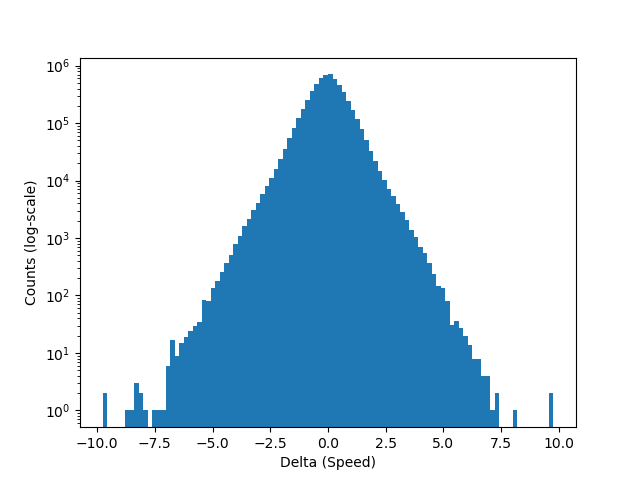
\includegraphics[width=0.6\linewidth]{figs/nedit_speed_distr.png}
  \vspace{0.1in}
  \label{fig:ne_speed_distr}
\end{figure*}

~\Cref{tab:neural-editor-eval} shows the results of training. We run all training scenarios three times and take the average. We find that all modifications significantly change the resulting $\Delta$ value while generally preserving lexical and semantic similarity. The variance across test samples is relatively low for each metric (\eg $0.005$ for BERTScore) so we only report the averaged metric. Unsurprisingly, when tolerance is low, we find good performance in $\Delta$ and poor performance in the similarity metrics. This result is likely due to overfitting from the lack of large amounts of training data. We see the strongest results with the Perturbation \& $\Delta$-Tolerance approaches, indicating that combining the two approaches is beneficial when the tolerance is tuned. 

At tolerance $\epsilon = 0.05$, including perturbed edit vectors improves the similarity metrics at the cost of $\Delta$, indicating that the perturbed approach may help combat overfitting. With tolerance $\epsilon = 0.1$, we see that perturbation is generally not helpful, and surprisingly, at tolerance $\epsilon = 0.2$, the perturbation approach leads to a higher $\Delta$. We hypothesize that at tolerance $\epsilon = 0.2$, there is an effective balance of constraint to a certain $\Delta$ and enough data for robust training. Further, the perturbation likely benefits from having $\Delta$-constrained pairs. We leave it to future work to investigate this behavior.

\begin{table}[h]
  \centering
  \small
  \caption{Evaluation metrics (BLEU \citep{Papineni2002bleu} and BERTScore \citep{zhang2019bertscore}) and strength of control on $\Delta$ for the trained models (ideally, $\Delta = 0.5$). The scores are averaged across three training runs with different seeds. We train a baseline model \citep{guu2018generating} (NeuralEditor Baseline), as well as multiple variants of the baseline. Neighborhood creation models are listed as ``Tol=$\epsilon$'' where $\epsilon$ is the tolerance. We also train a model following the edit vector perturbation approach and multiple models combining the two approaches. }
  \label{tab:neural-editor-eval}
  \begin{tabularx}{0.9\linewidth}{@{}>{\raggedright\arraybackslash}Xcccc@{}}
   \toprule[1.5pt]
  \textsc{Model} & \textsc{Delta} & \textsc{Train BLEU} & \textsc{Test BLEU} & \textsc{BERTScore} \\     
  \midrule[0.75pt]
  % \addlinespace[0.5em]
\textsc{NeuralEditor} Baseline    & 0.0113 & \textbf{0.6691}     & \textbf{0.5679}    & 0.9327 \\
  \midrule[0.75pt]
Tol=0.05               & 0.4559 & 0.8057     & 0.4266    & 0.9326 \\
Tol=0.1                & 0.4558 & 0.7146     & \textbf{0.5747}    & 0.9340 \\
Tol=0.2                & 0.4405 & 0.5994     & 0.5628    & 0.9355 \\
  \midrule[0.75pt]
Perturbation            & 0.4433 & 0.5513     & 0.4531    & 0.9346 \\
Perturbation + Tol=0.05 & 0.4279 & 0.5709     & 0.5218    & 0.9329 \\
Perturbation + Tol=0.1  & 0.4355 & 0.6375     & 0.5100    & 0.9386 \\
Perturbation + Tol=0.2  & \textbf{0.4596} & \textbf{0.6751}     & \textbf{0.5679}    & 0.9334 \\
  \bottomrule[1.5pt]\\
  \end{tabularx}
  \vspace{-10pt}
  \end{table}

\Cref{tab:ne_example} shows the generations of the \textsc{NeuralEditor} Baseline and each method with the tolerance at $0.2$. For both sequences, the generations of our modified models are much shorter while preserving content, indicating higher speed. The baseline for both prompts made minimal edits to the input sentences (\eg ``excellent'' to ``amazing''), resulting in close to no change in speed but an extremely high similarity. 

  \begin{table}[htb]
  \small
  \centering
  \caption{The baseline \citep{guu2018generating} (Prototype-then-Edit) as well as multiple variants of the baseline. Neighborhood creation models are listed as ``Tol=$\epsilon$'' where $\epsilon$ is the tolerance. The models are fed the input (\ie \textbf{Original}) and generate by applying an ``edit vector'' to the latent representation of the input sentence.}
  \label{tab:ne_example} 
  \begin{tabularx}{\linewidth}{@{}>{\raggedright\arraybackslash}X@{}}
   \toprule[1.5pt]
  \textsc{Model} \& \textsc{Generated Text}\\
  \midrule[0.75pt]
  \textsc{Example 1:}\\
  \textbf{Original}: He went above and beyond in providing us excellent customer service and was extremely courteous friendly and kind.  \\
  \textbf{\textsc{NeuralEditor} Baseline}: He went above and beyond in providing us with amazing customer service and was extremely courteous friendly and kind.  \\
  \textbf{Tol=0.2}: Always amazing customer service and very knowlegable staff. \\
  \textbf{Perturbation + Tol=0.2}: He was knowledgable, courteous, and went provided excellent customer service.\\
  \addlinespace[0.5em]
  \textsc{Example 2:}\\
  \textbf{Original}: The staff is very professional and friendly \& environment is clean.  \\
  \textbf{\textsc{NeuralEditor} Baseline}: The staff is very professional and likable \& the environment is clean. \\
  \textbf{Tol=0.2}: The friendly staff is very professional \& environment is clean. \\
  \textbf{Perturbation + Tol=0.2}: Friendly staff and clean environment.\\
  \bottomrule[1.5pt]\\
  \end{tabularx}
  \vspace{-10px}
  \end{table}

While the architecture shows a strong control over speed, it is hard to adjust our formulation to a wide range of controls. Neighborhood creation can easily be adapted for any control but severely restricts the amount of training data. Perturbation works well with constraints defined with word embeddings due to how the edit vector is constructed, but it likely will struggle with other controls. 

For traits like persuasiveness, we mainly enforce controls with a learned classifier or many smaller constraints (\eg speed). In the case of the former, this architecture would likely struggle because it would not have access to the learned weights. For the latter, having many constraints would limit the size of the training data and pollute the edit vector perturbation. We look to other models to resolve these issues.

In this section, we adapt the prototype-then-edit model proposed by \citet{guu2018generating} to controllable text generation. We show that our approach leads to significant control over speed while preserving relevance to the original text. In the next section, we modify the adversarial framework from~\Cref{chp:style_infusion} to control the speed of generated text and compare the results against this section's approach.

% Example 1
% he went above and beyond in providing us excellent customer service and was extremely courteous friendly and kind. 
% always amazing customer service and very knowlegable staff.
% he was knowledgable, courteous, and went provided excellent customer service.

% Example 2
% the staff is very professional and friendly & environment is clean.
% the friendly staff is very professional & environment is clean.
% friendly staff and clean environment.


\section{Adversarial Control}
\label{sec:adversarial_control}

In this section, we adapt the architecture proposed in Chapter \ref{chp:style_infusion} to encourage a pretrained sequence-to-sequence model to generate sentences with a specific change in speed through an adversarial training paradigm. In~\Cref{subsec:ac_data}, we describe the dataset used. Then in~\Cref{subsec:ac_attribute_regressor} we present an attribute regressor to predict speed, and in~\Cref{subsec:ac_model}, we plug in the regressor to the adversarial training framework to control speed. We describe the training process in~\Cref{subsec:ac_training} along with experiment settings, baselines, and metrics (\S\ref{subsec:ac_experimental}). Lastly, we present the results of our approach in~\Cref{subsec:ac_results}.

\subsection{Pairwise Data Generation}
\label{subsec:ac_data}

We utilize the Yelp Dataset\footnote{\url{https://www.yelp.com/dataset}} for this approach because many sentences are lexically similar (\ie within word-token Jaccard distance 0.5) but not repeated verbatim \citep{guu2018generating}. Since obtaining large amounts of pairwise data is hard, we create lexically similar pairs with a similar method to~\Cref{subsec:si_dataset}. For each sentence in the Yelp Dataset, we compute the top three similar sentences based on the Universal Sentence Encoder (USE) embeddings. For both sentences in the pair, we compute the speed, and the difference in speeds between the two, $\Delta = c' - c$, where $c'$ is the target speed, and $c$ is the original speed. 

\subsection{Attribute Regressor}
\label{subsec:ac_attribute_regressor}

We need a differentiable way to compute the relevant attribute to apply a constraint to the architecture from~\Cref{chp:style_infusion}. In the case of speed, the typical formulation is incompatible with PyTorch's backpropagation, so we train a language model to predict the direct speed of a sentence. We add a fully connected layer ($\mathbb{R}^d \rightarrow \mathbb{R}$, where $d$ is the hidden dimension) on top of a pre-trained LM. We use two models from the Huggingface Transformers library \citep{wolf2019}: \textit{bart-base} (12-layers, 768-dimensional) \citep{lewis2019bart} and \textit{roberta-base} (12-layers, 768-dimensional) \citep{liu2019roberta}. We train the entire model for five epochs with a batch size of 32 and $\eta = 5e-5$. Both architectures achieve a Mean Absolute Error (MAE) of approximately $0.073$ on a held-out test set.

\subsection{Architecture}
\label{subsec:ac_model}


% \begin{wrapfigure}{r}{0.5\textwidth}
%   \vspace{-0.35in}
%   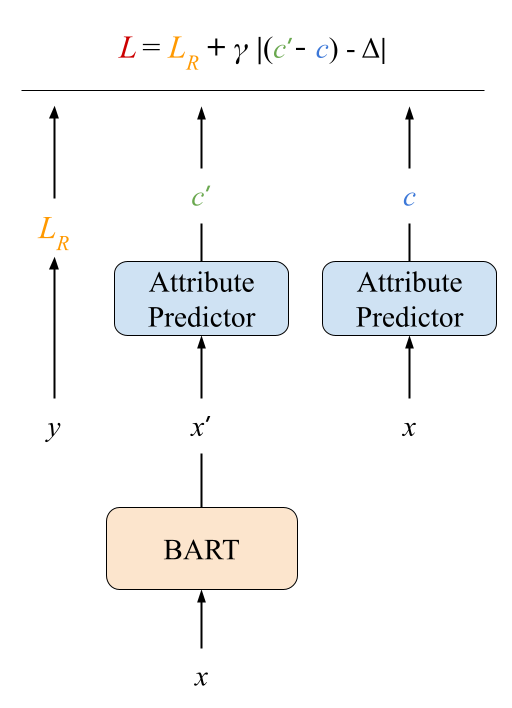
\includegraphics[width=0.9\linewidth]{figs/AC-Architecture.png}
%   \caption{Training diagram for adversarial control of an attribute (\eg speed). We compute the loss as a sum of the negative log likelihood ($L_R$) and the control tuning loss $L_C = \gamma |(c' - c) - \Delta|$.}
%   \label{fig:ac_architecture}
% \end{wrapfigure}

\begin{figure}
    \centering
    \caption{Training diagram for adversarial control of an attribute (\eg speed). We illustrate two approaches to enforce a control constraint via the input $x$: prepending a special token and adding an additional ``speed embedding''. In the latter approach, we add the speed embedding to every layer of BART to ensure information is not lost between encoder/decoder layers. We compute the loss as a weighted sum of the negative log-likelihood ($L_R$) and the control tuning loss $L_C = |(c' - c) - \Delta|$, where $\Delta$ is the desired change in speed. Note that we precompute $c$ to avoid unnecessary inference during training.}
    \label{fig:ac_architecture}
    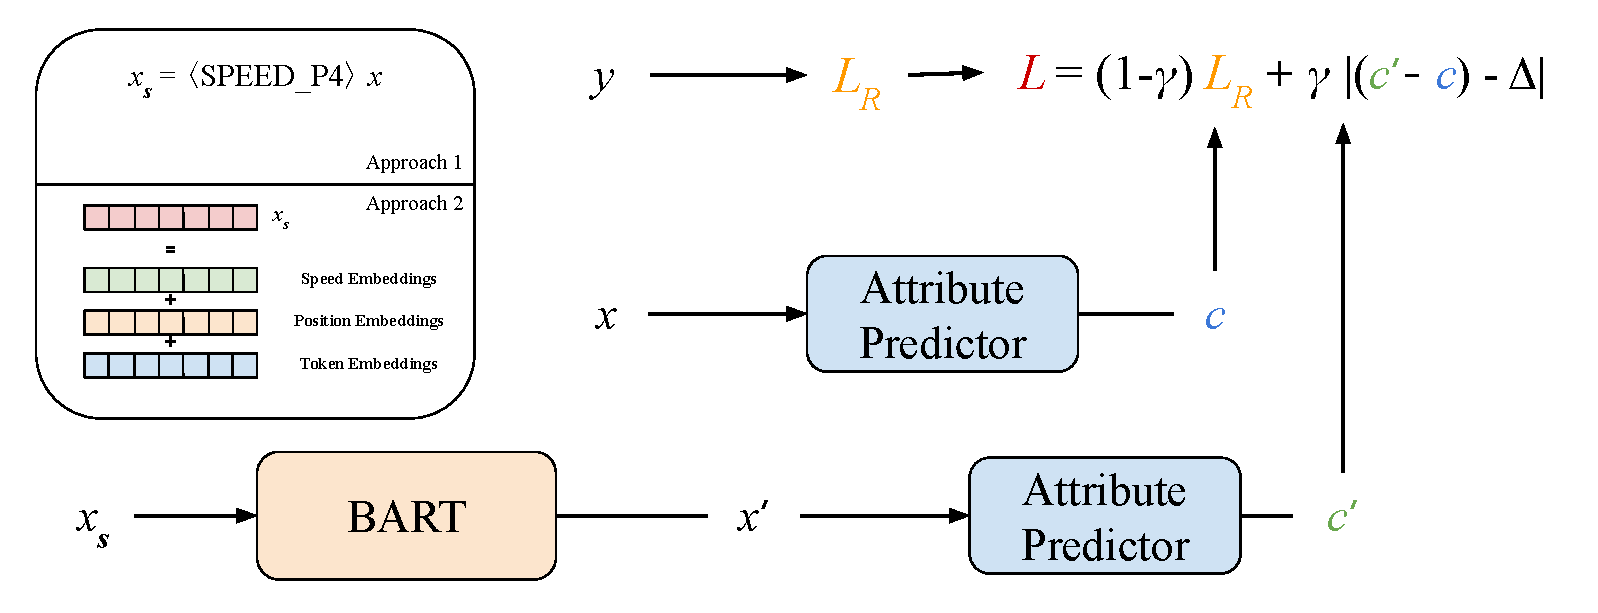
\includegraphics[width=\linewidth]{figs/AC-Architecture-H.pdf}
\end{figure}

In this section, we enforce controls learned by the attribute regressor in~\Cref{subsec:ac_attribute_regressor} into a sequence-to-sequence BART model. The architecture takes in an input sentence $x$ and a desired change in attribute, $\Delta$, generating an output sentence $x'$ that reflects the desired change in the attribute. However, we must modify BART to take $\Delta$ as an input to express the control. We try two methods: prepending a special token and adding a ``speed embedding'' to the token and positional embeddings, as well as in every encoder/decoder layer.

In the former approach, we quantize possible speed values into $2n + 1$ possible bins: $n$ for a positive change in speed, $n$ for a negative change in speed, and $1$ for no change in speed. We convert the bin into a special token containing the strength of change of speed and the direction (\eg ``$\langle$SPEED\_P4$\rangle$'' reflects a change in speed in the fourth highest bin). Each of the $n$ bins covers a range of speeds corresponding to an equal number of samples.

In the latter approach, we add a ``speed embedding'' vector to the token and positional embeddings in BART. The vector is the same size as the token embeddings and is filled with $\Delta$, the desired change in the attribute. We add the embedding vector after every encoder and decoder layer to ensure information is not lost between layers, and then batch normalization is applied.

We use a similar adversarial training paradigm to enable the generator to be controlled by the attribute classifier, illustrated in~\Cref{fig:ac_architecture}. 

\subsection{Training}
\label{subsec:ac_training}

We utilize two losses during training: a reconstruction loss, $L_R$, and a control tuning loss, $L_C$. The reconstruction loss maximizes the log probability of the original sentence, $y_s^*$.

\begin{equation}
    L_{R} = -\frac{1}{N} \sum_{i=1}^{N} \log p(y_s^{*(i)})
\end{equation}

The reconstruction loss teaches the model to mimic the gold-standard samples, preserving content. The control tuning loss enforces a target control and is formulated as follows:

\begin{equation}
    L_{C} = |(\mathcal{A}(x') - \mathcal{A}(x)) - \Delta|
\end{equation}

where $\Delta$ is the desired change in attribute (\eg speed) and $\mathcal{A}(\cdot)$ is the attribute classifier. During training, $x'$ is the first hidden state of the decoder (\ie the representation of the beginning of sequence token), and only the classifier head of the attribute regressor is used to compute the generated sequence's attribute. The final loss is a weighted sum of the two:

\begin{equation}
    L = (1-\gamma) L_R + \gamma L_C
\end{equation}

where $\gamma$ is a hyperparameter to weigh the effect of the control tuning loss and negative log-likelihood. 

\subsection{Experimental Settings}
\label{subsec:ac_experimental}

We train multiple variants of the modified architecture by modifying $\gamma$, the learning rate $\eta$, the attribute classifier architecture (\ie between BART and RoBERTa), and the control method (\ie between the special token and additional embedding methods). 

\textit{\textbf{Perturbation \& $\Delta$-Tolerance Baseline}} We utilize our approach from~\Cref{sec:neural_editor} as a strong baseline. For $\Delta$-Tolerance, we add a $\Delta$ constraint during neighborhood creation and train on the newly formed data. We try $\epsilon = \{0.05, 0.1, 0.2\}$ as tolerance values. For Perturbation, we add the $\Delta$-centered normal distribution to perturb the edit vector during training.

We utilize nucleus sampling to generate sentences with $p=0.8$ and include a repetition penalty \citep{keskar2019ctrl}. We record a few evaluation metrics to test the strength of the control as well as to ensure generations remain similar, lexically and semantically:

\textit{\textbf{METEOR}} We measure the METEOR (Metric for Evaluation of Translation with Explicit ORdering) score \citep{lavie-agarwal-2007-meteor}, essentially the harmonic mean for the test set. While we record BLEU for the previous approach, it will be artificially deflated in this comparison because we are not starting with a prototype. 

\textit{\textbf{BERTScore}} We measure the semantic similarity through the BERTScore \citep{zhang2019bertscore} to ensure that generations remain on topic.

\textit{\textbf{Mean Absolute Error (MAE)}} We record the mean absolute error between the target $\Delta$ and achieved $\Delta$.

\textit{\textbf{MAE From Bounds}} The special token approach for control quantizes speeds, making vanilla MAE an incomplete metric. We also compute the MAE of the generated text's $\Delta$ against the bounds of the respective target bin for speed. More formally, it is represented as 

\begin{equation}
    |\min(l - \Delta, u - \Delta)|
\end{equation}

where $l$ is the lower bound of the bin and $u$ is the upper bound of the bin.

\textit{\textbf{MAE From Center}} Similarly, we compute the MAE of the generated text's $\Delta$ against the mean of the respective target bin. We compute the mean using the $\Delta$s of the training samples instead of directly using $u$ and $l$. 

\subsection{Results}
\label{subsec:ac_results}

% Alter attribute classifier
\begin{table}[]
\centering
\small
\caption{Evaluation metrics for lexical similarity (METEOR \citep{lavie-agarwal-2007-meteor}), semantical similarity (BERTScore \citep{zhang2019bertscore}), and strength of control on $\Delta$, measured with Mean Absolute Error (MAE), MAE from Bounds (MAE-B), and MAE from Center (MAE-C). We compare both the token-based control and the embedding-based control across two different attribute classifier architectures - BART \citep{lewis2019bart}, and RoBERTa \citep{liu2019roberta} - denoted by $\mathcal{A}$. We compare these approaches against the Perturbation \& $\Delta$-Tolerance Baseline from~\Cref{sec:neural_editor}. All of our approaches from this section are trained with $\eta=5e-5$ and $\gamma=0.1$.}
\label{tab:ac_model_variation}

\begin{tabularx}{\linewidth}{@{\extracolsep{\fill}} ccccccc}
\toprule[1.5pt]
                               & $\mathcal{A}$   & \textsc{MAE}    & \textsc{MAE-B} & \textsc{MAE-C} & \textsc{METEOR} & \textsc{BERTScore} \\
\midrule[0.75pt]
Perturb + Tol=0.05             & -               & 0.0721          & -              & -              & 0.5123          & 0.9326 \\
Perturb + Tol=0.1              & -               & 0.0645          & -              & -              & 0.4993          & \textbf{0.9386} \\
Perturb + Tol=0.2              & -               & \textbf{0.0404} & -              & -              & \textbf{0.5391} & 0.9334 \\
\midrule[0.75pt]
\multicolumn{1}{c}{Token}      & BART            & 0.2918          & 0.2136          & 0.2886          & 0.1633          & 0.8710  \\
                               & RoBERTa         & 0.2193          & 0.1405          & 0.2174          & 0.1605          & 0.8749  \\
\midrule[0.75pt]
\multicolumn{1}{c}{Embedding}  & BART            & 0.2819          & -              & -              & 0.1724          & 0.8728  \\
                               & RoBERTa         & 0.2187          & -              & -              & 0.1515          & 0.8728  \\
  \bottomrule[1.5pt]\\
\end{tabularx}
\end{table}

We present the results of our approach in~\Cref{tab:ac_model_variation},~\Cref{tab:ac_lr_variation}, and~\Cref{tab:ac_gamma_variation}, with the former having varied attribute classifier architectures and the latter two having varied learning rates and values of $\gamma$, respectively. The variance across test samples is relatively low for each metric (\eg $0.005$ for BERTScore and $0.03$ for METEOR), so we only report the averaged metric. Our results show that despite the variations of our approach, it fails to outperform our approach from~\Cref{sec:neural_editor}. While lexical and semantical similarity scores are lower than the baseline, this is expected from a larger neural model that is not trained to ``prototype''. However, the metrics for control of speed show that it is difficult for the model to exhibit fine-grained control.

In~\Cref{tab:ac_model_variation}, we find that RoBERTa is significantly stronger than BART in the case of the special token approach, while both are approximately equal in the embedding approach. The decoder layers in BART are likely unnecessary for predicting speed, making RoBERTa more efficient. However, both achieved similar performance on a held-out test set, as mentioned in~\Cref{subsec:ac_attribute_regressor}, implying that RoBERTa developed more robust representations that were transferred during the adversarial training. 

% Alter Learning rate table
\begin{table}[]
\centering
\small
\caption{Evaluation metrics for lexical similarity (METEOR \citep{lavie-agarwal-2007-meteor}), semantical similarity (BERTScore \citep{zhang2019bertscore}), and strength of control on $\Delta$, measured with Mean Absolute Error (MAE), MAE from Bounds (MAE-B), and MAE from Center(MAE-C). We compare the token-based and embedding-based control across three learning rates ($\eta$). We compare these approaches against the Perturbation \& $\Delta$-Tolerance Baseline from~\Cref{sec:neural_editor}. All of our approaches from this section are trained with $\mathcal{A}$ as RoBERTa and $\gamma=0.1$.}
\label{tab:ac_lr_variation}

% 
\begin{tabularx}{\linewidth}{@{\extracolsep{\fill}} ccccccc}
\toprule[1.5pt]
                              & $\eta$           & \textsc{MAE}    & \textsc{MAE-B} & \textsc{MAE-C} & \textsc{METEOR} & \textsc{BERTScore} \\
\midrule[0.75pt]
Perturb + Tol=0.05            & -                & 0.0721          & -              & -              & 0.5123          & 0.9326 \\
Perturb + Tol=0.1             & -                & 0.0645          & -              & -              & 0.4993          & \textbf{0.9386} \\
Perturb + Tol=0.2             & -                & \textbf{0.0404} & -              & -              & \textbf{0.5391} & 0.9334 \\
\midrule[0.75pt]
                              & 1e-5      & 0.3149          & 0.2361         & 0.3111         & 0.1566          & 0.8746  \\
\multicolumn{1}{c}{Token}     & 5e-5      & 0.2193          & 0.1405         & 0.2172         & 0.1605          & 0.8749  \\
                              & 1e-6      & 0.2539          & 0.1754         & 0.2516         & 0.1898          & 0.8710  \\
\midrule[0.75pt]
                              & 1e-5      & 1.7268          & -              & -              & 0.1278          & 0.8721  \\
\multicolumn{1}{c}{Embedding} & 5e-5      & 0.2187          & -              & -              & 0.1515          & 0.8728  \\
                              & 1e-6      & 0.2182          & -              & -              & 0.1724          & 0.8687  \\
  \bottomrule[1.5pt]\\
\end{tabularx}
\end{table}

In~\Cref{tab:ac_lr_variation}, we find an optimal learning rate of $\eta = 5e-5$, which strongly outperforms the other models. Both tables clearly show that the special token-based approach outperforms the embedding-based approach. This result is likely because the special token encodes more information than the uniform embedding, which is confounded with the positional and token embeddings. One exciting avenue for future work is to add the ``control embedding'' to disentangle all three embeddings similarly to \citet{he2020deberta}. 

In~\Cref{tab:ac_gamma_variation}, we vary the value of $\gamma$ across the token-based control. $\gamma=0$ (\ie fine-tuning on our training data) behaves as expected with high lexical and semantic similarity scores, relative to the other values of $\gamma$, but poor control over speed. Empirically, $\gamma = 0.1$ was the strongest approach, balancing control over speed and similarity to the target text. The embedding-based control did not exhibit a significant difference when $\gamma$ was altered; thus, we omitted it from the table.

% Alter gamma table
\begin{table}[]
\centering
\small
\caption{Evaluation metrics for lexical similarity (METEOR \citep{lavie-agarwal-2007-meteor}), semantical similarity (BERTScore \citep{zhang2019bertscore}), and strength of control on $\Delta$, measured with Mean Absolute Error (MAE), MAE from Bounds (MAE-B), and MAE from Center(MAE-C). We compare the token-based control across three different values of $\gamma$. We compare these approaches against the Perturbation \& $\Delta$-Tolerance Baseline from~\Cref{sec:neural_editor}. All of our approaches from this section are trained with $\mathcal{A}$ as RoBERTa and $\eta=5e-5$.}
\label{tab:ac_gamma_variation}

\begin{tabularx}{\linewidth}{@{\extracolsep{\fill}} ccccccc}
\toprule[1.5pt]
                              & $\gamma$           & \textsc{MAE}    & \textsc{MAE-B} & \textsc{MAE-C} & \textsc{METEOR} & \textsc{BERTScore} \\
\midrule[0.75pt]
Perturb + Tol=0.05            & -                & 0.0721          & -              & -              & 0.5123          & 0.9326 \\
Perturb + Tol=0.1             & -                & 0.0645          & -              & -              & 0.4993          & \textbf{0.9386} \\
Perturb + Tol=0.2             & -                & \textbf{0.0404} & -              & -              & \textbf{0.5391} & 0.9334 \\
\midrule[0.75pt]
                              & 0.0              & 0.5051          & 0.4282         & 0.4889         & 0.1724          & 0.8877  \\
\multicolumn{1}{c}{Token}     & 0.1              & 0.2193          & 0.1405         & 0.2172         & 0.1605          & 0.8749  \\
                              & 0.2              & 0.2517          & 0.1730         & 0.2492         & 0.1655          & 0.8710  \\
                              & 0.5              & 0.3304          & 0.2501         & 0.3251         & 0.1446          & 0.8746  \\
  \bottomrule[1.5pt]\\
\end{tabularx}
\end{table}

\Cref{tab:ac_example} shows the generations of the baselines of the previous approach (\S\ref{sec:neural_editor}) and $\gamma$-variants of the adversarial training approach. We find that while all generations are generally fluent and on topic, the change in speed of the baseline approach, $\gamma=0.1$, and $\gamma=0.2$ are more positive than the other approaches, as they tend to cover more content in a shorter time frame. However, it is interesting that the generations of $\gamma=0.0$ are similar to, if not the same as, generations from models with the control tuning loss. We also notice that this approach tends to hallucinate some details. For example, for the input ``He went above and beyond in providing us excellent customer service and was extremely courteous friendly and kind,'' the model generates ``The service was great, the gentleman who helped us was very friendly and helpful. \textit{He made sure we were happy with our purchase},'' incorrectly implying the reviewer made a purchase. However, this is a common problem in existing generation models \citep{ji2022survey}, and we leave it to future work to explore this issue in depth.

  \begin{table}[htb]
  \small
  \centering
  \caption{The previous section's approach (Perturbation + Tol=0.2) along with variants of our adversarial training approach. Neighborhood creation models are listed as ``Tol=$\epsilon$'' where $\epsilon$ is the tolerance. The adversarially-trained models are all trained with the Token-based method, RoBERTa as $\mathcal{A}$, and $\eta=5e-5$ as they are empirically the best settings. We vary the value of $\gamma$ to test the impact of the control tuning loss. The models are fed the input (\ie \textbf{Original}) with a target $\Delta=0.5$ and either generate by applying an ``edit vector'' to the latent representation of the input or through nucleus sampling with $p=0.8$.}
  \label{tab:ac_example} 
  \begin{tabularx}{\linewidth}{@{}>{\raggedright\arraybackslash}X@{}}
   \toprule[1.5pt]
  \textsc{Model} \& \textsc{Generated Text}\\
  \midrule[0.75pt]
  \textsc{Example 1:}\\
  \textbf{Original}: He went above and beyond in providing us excellent customer service and was extremely courteous friendly and kind.  \\
  \textbf{Perturbation + Tol=0.2}: He was knowledgable, courteous, and went provided excellent customer service.\\
  \textbf{Ours ($\gamma=0.0$)}: The service was great. The gentleman who helped us was very friendly and helpful, but not pushy at all.\\
  \textbf{Ours ($\gamma=0.1$)}:  The service was great, the gentleman who helped us was very friendly and helpful. He made sure we were happy with our purchase!\\
  \textbf{Ours ($\gamma=0.2$)}:  The service was prompt and friendly and the food delicious.  Also cheap as hell.\\
  \textbf{Ours ($\gamma=0.5$)}: He was very friendly and helpful. He made our experience a great one! Thank you for being such an amazing customer service!! \\
  \addlinespace[0.5em]
  \textsc{Example 2:}\\
  \textbf{Original}: The staff is very professional and friendly \& environment is clean.  \\
  \textbf{Perturbation + Tol=0.2}: Friendly staff and clean environment.\\
  \textbf{Ours ($\gamma=0.0$)}: The staff is very friendly and helpful. \\
  \textbf{Ours ($\gamma=0.1$)}: The staff is very friendly and helpful. \\
  \textbf{Ours ($\gamma=0.2$)}:  The staff is friendly.\\
  \textbf{Ours ($\gamma=0.5$)}:  The staff is very friendly and professional.  The place is clean, well kept and the environment was nice as well!\\
  \bottomrule[1.5pt]\\
  \end{tabularx}
  \vspace{-10px}
  \end{table}

While the approach was relatively successful in some settings, fine-tuning the entire BART model may be unnecessarily expensive and degrade generation quality. \citet{li2021prefix} propose a lightweight alternative that optimizes the prefix, a relatively small, task-specific, continuous vector prepended to the input. By learning a small fraction of the parameters of the entire model, prefix-tuning capitalizes on extensive pretraining while outperforming other baselines in task-specific settings. Initial experiments have shown some promise, but we want to continue exploring this direction for lightweight, controllable text generation techniques. We also leave it to future work to discover methods for multiple constraints and to empirically investigate existing formulations that allow for more than one control.

In this section, we propose an adversarial training framework to control the speed of generated text and show that our approach exhibits decent control over speed. We propose a few avenues to improve this exploratory work which we plan to continue investigating.

\section{Conclusion}
\label{sec:ctrl_conclusion}

In this chapter, we propose two separate approaches to controllable text generation for complex linguistic features: modifications to the prototype-then-edit framework \citep{guu2018generating} and an adversarial framework with an attribute regressor to control target features. Through various evaluation metrics, we show that both approaches result in fluent, relevant, and controlled generations and propose multiple directions for future work. In the next chapter, we conclude this thesis and discuss the limitations of this thesis as well as the ethical considerations of our work.

\chapter{Conclusions}
\label{chp:concl}
% \section{Conclusion}
% p1 summarize findings p2 consequences/impact
This thesis investigates how to synthesize persuasive content through a combination of state-of-the-art natural language generation techniques and theoretical constructs from advertising and journalism. 

In~\Cref{chp:style_infusion}, we introduced \textit{style infusion} to motivate infusing audience-centric, stylistic preferences into unconstrained natural language generation models. We present a bootstrapped data augmentation method for limited pair-wise audience feedback and an adversarial training framework with a decoupling loss to train a style-infused GPT-2. Through an automatic evaluation method for the transfer of audience-specific styles, we show that our approach generates compelling stylized examples with generic text prompts better than the baselines. 

In~\Cref{chp:control_gen}, we experiment with novel approaches for controllable natural language generation to condition text on a "tuning-knob" for target controls (\eg speed). We present a modified prototype-then-edit model \citep{guu2018generating} and empirically show that our modifications lead to a substantial control on speed. We then alter our architecture from~\Cref{chp:style_infusion} to adversarially enforce a desired change in speed, finding that it can control speed, although less strongly than the previous approach.

Synthesizing text with highly subjective styles, such as persuasion and memorability, remains a significant challenge in domains like computational advertising. Our work takes the first few steps to address this problem, and we hope to inspire future research on this topic with this thesis. Ultimately, we aspire for the persuasive text generation systems we develop to be used with abstractive summarization techniques for scientific literature to generate more approachable and appealing science communication.

We mention the limitations of our work in~\Cref{sec:limitations} and then address the ethical implications of this thesis in~\Cref{sec:ethics}.

\section{Limitations}
\label{sec:limitations}

As with other unconstrained natural language generation applications, our systems are prone to issues like degeneration from beam search and neural hallucinations \citep{ji2022survey}. We post-process generations to combat the former problem, but future work will hopefully provide better methods to prevent this issue. The latter primarily applies to~\Cref{chp:style_infusion}, in which we increase our dataset with samples from the CNN/DailyMail dataset \citep{see-etal-2017-get}, partially mitigating the problem, but out-of-domain topics still suffer. Expanding the dataset size will only work for so long due to diminishing marginal returns.

We also note that our frameworks are limited by the computational resources available to us. Thus, we could not effectively support long text generation while preserving the quality of the generated text. During training, we decreased the batch size and utilized the DeepSpeed framework \citep{rasley-2020-deepspeed}, but it is still insufficient to handle long text. Furthermore, traditional left-to-right generation struggles with long text as the topics tend to diverge \citep{Tan2020}. Because many styles, like persuasiveness, depend on paragraph-level features in addition to sentence-level features, it is beneficial for our application to support longer texts.

Due to the limited data available for our style infusion approach, we considered iteratively training the discriminator with the augmented data while we trained the generator. Ultimately, we felt that the weak labels would dilute the learned trends in the discriminator, but it may be interesting to see how it affects the framework's performance. Currently, collecting pairwise datasets to use with this framework can be considered a limitation. With increasing interest in the computational synthesis of persuasive text and imagery, we expect to see more relevant curated datasets in the near future. Generating pairwise data through human subject experiments is expensive, which is why the data augmentation methods introduced in this paper are crucial for future work. We also note that while we claim that humans are better at pairwise evaluations, recent work has shown that humans are not always the gold standard for labeling, especially in natural language generation tasks \citep{clark2021all}.

One of the most significant limitations of the style infusion approach is in showing the effectiveness of our chosen architecture. Because most baselines are in style transfer and fundamentally differ from our task, we find it difficult to make a fair comparison with prior work. Regardless, style infusion is a critical step for unconstrained NLG systems such as dialogue systems and chatbots, especially in the context of human-centric stylistic objectives, which are already difficult enough to define. We encounter similar challenges in our work on stylized controllable text generation because many existing architectures do not generalize well and produce poor results. 

As mentioned in~\Cref{subsec:ne_results}, the modified prototype-then-edit model for controllable text generation is limited by its formulation. While it produces good results for speed, it will likely struggle with other constraints due to how the edit vector is constructed and requires expensive retraining for different values of $\Delta$. Conversely, the adversarial architecture in~\Cref{sec:adversarial_control} is likely able to adapt well to other constraints and can exhibit control on any arbitrary value of $\Delta$. However, neither of our current formulations would allow for the control of multiple constraints simultaneously, eliminating them as candidates for controlling styles that depend on the composition of features (\eg persuasiveness). 






\section{Ethics Statement}
\label{sec:ethics}

Our objective for developing controllable stylistic generative language models that leverages domain and audience-specific feedback is to enable unconstrained generation applications to appeal to more human users. For example, generating more persuasive real news might help combat misinformation by propagating the truth faster than falsehoods. In advertising and communication, persuasiveness and memorability are critical traits, and having an unconstrained generation model that could replicate these features would have a multitude of positive applications, especially in targeted interventions. Previous research has focused chiefly on predicting audience characteristics and targeting rather than synthesizing matching messages.

We acknowledge the dual-use concerns of the misuse of such a generation framework to, for example, spread misinformation. For this reason, we do not release the models or the pretrained generator checkpoints used in this work. 



  % Inserts content from "conclusion.tex" here

\chapter{Future Directions}
\label{chp:future}
We plan to continue improving our work in many directions to achieve persuasive text-generation systems that make scientific literature more approachable and appealing to the general public. Primarily, we aim to run multiple human subject evaluation studies to ensure that our proposed approaches lead to fluent, relevant, and stylized or controlled generations. We also look to the following areas as promising avenues for future work:

\begin{itemize}
    \item \textbf{Abstractive Summarization}: Studies have shown that the dissemination of scientific literature is strongly correlated with sharing work through social media (\eg Twitter) \citep{eysenbach2011can, tahamtan2016factors}. \citet{eysenbach2011can} find that research tweeted about frequently in the first few days following publications was 11 times more likely to be highly cited than less tweeted articles. By utilizing abstractive summarization techniques for scientific literature \citep{cohan2018discourse, altmami2020automatic}, we hope to help scientists share their findings and encourage the direct dissemination of scientific information.

    \item \textbf{Discourse Structure}: Despite scientific news articles conveying similar information to scientific literature, the former tends to be more appealing to a layperson audience \citep{plaven2017research}. Studies have found that news articles often follow an inverted pyramid structure while scientific literature follows its own structure \citep{rafiee2018culture, cohan2018discourse}. We hypothesize that the discourse structure plays a significant role in ordering how ideas are conveyed and capturing the attention of target audiences. We hope to generate more appealing texts by altering the discourse structure while presenting the same content.
    
    \item \textbf{Long-text Processing \& Generation}: Scientific texts tend to be long \citep{tretyak2020combination} and infeasible to process with vanilla transformers \citep{vaswani2017attention} due to memory and computational requirements growing quadratically with sequence length. Furthermore, vanilla transformers struggle to remember long-term dependencies when generating text, leading to incoherent and contradictory texts. Potential solutions include incorporating long-document attention mechanisms \citep{beltagy2020longformer, zaheer2020big} to capture document-level style features and using progressive generation, instead of planning-then-generation, to improve long-document generation quality \citep{Tan2020}.
    
    \item \textbf{Knowledge-Driven Natural Language Generation}: Existing large language models are prone to neural hallucinations \citep{ji2022survey}, which can be extremely dangerous for persuasive systems for scientific literature. Existing methods have explored ways to incorporate external knowledge structures into text generation \citep{yu2022survey, wang2019paperrobot}, and we hope to utilize these works to ensure the factuality of our generations.
\end{itemize}

\ctparttext{
    \lipsum[3]
}
%\addtocontents{toc}{\protect\clearpage} % <--- just debug stuff, ignore
% \include{Chapters/Chapter03}
%\include{multiToC} % <--- just debug stuff, ignore for your documents
% ********************************************************************
% Backmatter
%*******************************************************
\appendix
%\renewcommand{\thechapter}{\alph{chapter}}
\cleardoublepage
\chapter{Appendix}
\part{Feature Agreement}
\label{apx:featureagreement}

% Persuasiveness Correlation Results
\begin{table*}[ht!]
\caption{\label{tab:feature-evaluation}Significance tests on the change in features between a pretrained GPT-2 model and a trained model. In order, these features are: Brunet Index (BI), Length (in characters), Total Dependencies (TD), Total Dependency Distance (TDD), Average Syllables per Word, Flesh-Kincaid readability score, Ratio of Jargon (i.e. out of vocab words), Flesch readability score, Token Type Ratio (TTR), Ratio of Present Tense Verbs, Speed, and Volume. In the table, the number of checks or crosses indicates the level of p-value and the correctness of the direction of the trend. Note that \cmark : $p < 0.05$, \ccmark : $p < 0.01$, \cccmark : $p < 0.001$, \ccccmark : $p < 0.0001$.}
\scalebox{0.7}{
\begin{tabular}{|l|cccccc|cccccc|}
\hline
Model    & BI                                            & Length                                        & TD                                            & TDD                                           & Syllables           & Flesch-Kincaid                        & Jargon       & Flesch                                        & TTR                                   & Present                                       & Speed                                 & Volume                                \\ \hline
GPT2     & -                                             & -                                             & -                                             & -                                             & -                   & -                                     & -            & -                                             & -                                     & -                                             & -                                     & -                                     \\
GPT2-16k & \cmark                                  & \xxxxmark         & \xxxxmark         & -                                             & -                   & -                                     & \xmark & -                                             & \ccmark                   & \xxxxmark & -                                     & \ccccmark \\
GPT2-Aug & \ccccmark & \ccccmark & \cmark                                  & \ccccmark & -                   & \xxxxmark & -            & \xxxxmark & \cmark                            & -                                             & \ccccmark & \ccmark                   \\
TStylist & \cmark & \ccccmark & \cccmark                                  & - & \ccmark                   & \xxxxmark & \xxxxmark            & \xxxxmark & \cmark                            & -                                             & \cccmark & \cccmark                   \\ \hline
AP-0.1   & \ccccmark & \ccccmark & \ccmark                       & \ccccmark & -                   & \xxxxmark & -            & \xxxxmark & \ccmark                   & \cmark                                    & \ccmark                   & \cccmark          \\
AP-1.0   & \ccccmark & \ccccmark & \cmark                                  & \ccccmark & -                   & \xxxxmark & -            & \xxxxmark & \ccmark                   & -                                             & \cccmark          & \ccccmark \\
SD-0.1  & -                                             & -                                             & \cmark                                  & -                                             & \xxmark & \xxxxmark & -            & \xxxxmark & \xmark                          & -                                             & \cmark                            & -                                     \\
SD-0.5  & \ccccmark & \ccccmark & \ccccmark & \ccccmark & -                   & -                                     & -            & \xmark                                  & \ccccmark & \ccccmark         & \ccccmark & \ccccmark \\
SD-0.8  & -                                             & \ccccmark & \ccccmark & \cmark                                  & -                   & \xxmark                   & -            & \xxxmark            & \ccmark                   & \cmark                                    & \ccccmark & \ccccmark \\
SD-1.0  & \ccccmark & \ccccmark & \ccccmark & \cccmark            & \xmark          & -                                     & -            & -                                             & \ccccmark & \ccccmark         & \ccccmark & \ccccmark \\ \hline
\end{tabular}}
\end{table*}

% Memorability Correlation Results
\begin{table*}[ht!]
\caption{\label{tab:mem-feature-evaluation}Significance tests on the change in features between a pretrained GPT-2 model and a trained model. In order, these features are: Length (in characters), Brunet Index (BI), Total Dependency Distance (TDD), Total Dependencies (TD), Circuitousness, Punctuation Rate, Past, Pronoun Rate, Closed Class Word (CCW) Rate, Token Type (TTR) Ratio, Average Dependency Distance (ADD), Average Dependencies (AD). In the table, the number of checks or crosses indicates the level of p-value and the correctness of the direction of the trend. Note that \cmark : $p < 0.05$, \ccmark : $p < 0.01$, \cccmark : $p < 0.001$, \ccccmark : $p < 0.0001$.}
\scalebox{0.65}{
\begin{tabular}{|l|cccccc|cccccc|}
\hline
Model    & Length                                            & BI                                        & TDD                                            & TD                                           & Circuitousness           & PunctRate                        & Past       & Pronoun Rate                                        & CCW Rate                                   & TTR                                       & ADD                                 & AD                                \\ \hline
GPT2     & -                                             & -                                             & -                                             & -                                             & -                   & -                                     & -            & -                                             & -                                     & -                                             & -                                     & -                                     \\
GPT2-IMDB & - & \ccccmark                                 & \xxmark & - & \xmark                   & \cmark & \cccmark            & \xxxxmark & \ccccmark                            & -                                             & \ccccmark & \ccccmark                   \\
GPT2-Aug & \ccccmark & \ccccmark                                  & \ccccmark & \ccccmark & \ccccmark                   & \cmark & \ccccmark            & \xxxxmark & \xxxxmark                            & \ccccmark                                             & \xxxxmark & \xxxxmark                   \\ 
TStylist & \ccccmark & \ccccmark & \cccmark & \cccmark & \cccmark & \cmark & \ccccmark & \xxxmark & - & \ccccmark & \xxxmark & \ccccmark \\\hline
AP-0.1 & \ccccmark & \ccccmark & \ccccmark & \ccccmark & \ccccmark & - & \ccccmark & \xxxxmark & \xxxxmark & \ccccmark & \xxxxmark & \xxxxmark  \\
AP-1.0 & \ccccmark & \ccccmark & \ccccmark & \ccccmark & \ccccmark & - & \ccccmark & \xxxxmark & \xxxxmark & \ccccmark & \xxxxmark & \xxxxmark  \\
SD-0.1 & \ccccmark & \ccccmark & \ccccmark & \ccccmark & \ccccmark & - & \ccccmark & \xxxxmark & \xxxmark & \ccccmark & \xxxxmark & \xxxxmark  \\
SD-0.5   & \ccccmark & \ccccmark                                  & \ccccmark & \ccccmark & \ccccmark                   & \cmark & \ccccmark            & \xxxmark & \ccccmark                            & \ccccmark                                             & \ccmark & \ccccmark  \\
SD-0.8 & \ccccmark & \ccccmark & \ccccmark & \ccccmark & \ccccmark & - & \ccccmark & \xxxxmark & \xxmark & \ccccmark & \xxxxmark & \xxxxmark  \\
SD-1.0  & \ccccmark & \ccccmark                                  & \ccccmark & \ccccmark & \ccccmark                   & \ccmark & \ccccmark            & \xxxxmark & \cccmark                            & \ccccmark                                             & \cmark & \ccccmark  \\ \hline
\end{tabular}}
\end{table*}

To demonstrate feature agreements, we calculate a weighted average to quantify the results of~\Cref{tab:feature-evaluation} in the context of the full feature set, using the correlations obtained from the Bayesian model as weights. The results are shown in~\Cref{tab:agreement-evaluation}. 

  \begin{table*}[ht!]
  \centering
  \caption{Percentage agreement with the linguistic feature correlations calculated using the hierarchical Bayesian model. Baseline models: GPT2, GPT-2 fine-tuned on UKPConvArg1 or the Cornell Movie Quotes corpus, GPT-2 with augmented data, and TitleStylist \citep{jin2020hooks}. Our models are trained on augmented data and a sample-dependent discriminator (SD) or sample-dependent supervised (SS) loss with parameter $\beta$. We show that our models are significantly better at learning stylistic features compared to our baselines.}
  \label{tab:agreement-evaluation}
  \scalebox{0.8}{
  \begin{tabularx}{0.6\linewidth}{@{}>{\raggedright\arraybackslash}Xccc@{}}
   \toprule[1.5pt]
  \textsc{Model} & \textsc{Persuasiveness}            & \textsc{Memorability}   \\     
  \midrule[0.75pt]
GPT2     & 29.51          & 40.71                 \\
GPT2-FT  & 41.03          & 46.22                  \\
GPT2-Aug & 44.01          & 51.26                \\
TStylist & 35.76          & 43.86                   \\
  \midrule[0.75pt]
  % \addlinespace[0.5em]
SS-0.1   & 42.26          & 49.70                \\
SS-1.0   & 48.57          & 44.97                   \\
SD-0.1  & 43.58          & 48.73                 \\
SD-0.5  & 48.56          & \textbf{62.35} \\
SD-0.8  & 50.04          & 48.14              \\
SD-1.0  & \textbf{50.18}          & 55.61                   \\
  \bottomrule[1.5pt]\\
  \end{tabularx}}
  \end{table*}

\part{Collected Linguistic Features}
\label{apx:lfc}

We collected the following linguistic features: length, verb tenses (e.g. future, past, etc.), punctuation rates, readability scores (Flesch score, Flesch-Kincaid score, Gunning Fog score, SMOG score, Dale-Chall score), part of speech rates (noun rate, verb rate, demonstrative rate, adjective rate, adposition rate, adverb rate, auxiliary rate, conjunction rate, determiner rate, interjection rate, numeral rate, particle rate, pronoun rate, proper noun rate, punctuation rate, subordinating conjunction rate, symbol rate, possessive rate), ratios of part of speech (e.g. noun-verb ratio, noun ratio, pronoun-noun ratio, closed-class word rate, open-class word rate), dependency information (total dependency distance, average dependency distance, total dependencies, average dependencies),  content density, idea density, lexical diversity statistics (Honore statistic, Brunet index), type token ratio, average word length, proportion of inflected verbs, proportion of auxiliary verbs, proportion of gerund verbs, proportion of participles, proportion of mispelled words, amount of alliteration, passive voice, average number of syllables, proportion of jargon, proportion of MTCG verbs (Modal, Tentative, Certainty, Generalizing), rates of named-entity recognition (NER) tags (e.g. PERSON, DATE, CARDINAL, WORK OF ART, NORP, Certainty, GPE, ORG, LOC, PERCENT, MONEY, QUANTITY, TIME, PRODUCT, EVENT, LANGUAGE, FAC), and word embedding-based measures (i.e. speed, volume, circuitousness) \citep{toubia-2021}. The NER tags were obtained from the spaCy library \citep{spacy2} and many of the linguistic features are obtained from the blabla library \citep{shivkumar2020blabla}.

%********************************************************************
% Other Stuff in the Back
%*******************************************************
\cleardoublepage%********************************************************************
% Bibliography
%*******************************************************
% work-around to have small caps also here in the headline
% https://tex.stackexchange.com/questions/188126/wrong-header-in-bibliography-classicthesis
% Thanks to Enrico Gregorio
\defbibheading{bibintoc}[\bibname]{%
  \phantomsection
  \manualmark
  \markboth{\spacedlowsmallcaps{#1}}{\spacedlowsmallcaps{#1}}%
  \addtocontents{toc}{\protect\vspace{\beforebibskip}}%
  \addcontentsline{toc}{chapter}{\tocEntry{#1}}%
  \chapter*{#1}%
}
\printbibliography[heading=bibintoc]

% Old version, will be removed later
% work-around to have small caps also here in the headline
%\manualmark
%\markboth{\spacedlowsmallcaps{\bibname}}{\spacedlowsmallcaps{\bibname}} % work-around to have small caps also
%\phantomsection
%\refstepcounter{dummy}
%\addtocontents{toc}{\protect\vspace{\beforebibskip}} % to have the bib a bit from the rest in the toc
%\addcontentsline{toc}{chapter}{\tocEntry{\bibname}}
%\label{app:bibliography}
%\printbibliography

% \cleardoublepage%*******************************************************
% Declaration
%*******************************************************
\pdfbookmark[0]{Declaration}{declaration}
\chapter*{Declaration}
\thispagestyle{empty}
Put your declaration here.
\bigskip

\noindent\textit{\myLocation, \myTime}

\smallskip

\begin{flushright}
    \begin{tabular}{m{5cm}}
        \\ \hline
        \centering\myName \\
    \end{tabular}
\end{flushright}

% \cleardoublepage\pagestyle{empty}

\hfill

\vfill


\pdfbookmark[0]{Colophon}{colophon}
\section*{Colophon}
This document was typeset using the typographical look-and-feel \texttt{classicthesis} developed by Andr\'e Miede and Ivo Pletikosić.
The style was inspired by Robert Bringhurst's seminal book on typography ``\emph{The Elements of Typographic Style}''.
\texttt{classicthesis} is available for both \LaTeX\ and \mLyX:
\begin{center}
\url{https://bitbucket.org/amiede/classicthesis/}
\end{center}
Happy users of \texttt{classicthesis} usually send a real postcard to the author, a collection of postcards received so far is featured here:
\begin{center}
\url{http://postcards.miede.de/}
\end{center}
Thank you very much for your feedback and contribution.

\bigskip

\noindent\finalVersionString

%Hermann Zapf's \emph{Palatino} and \emph{Euler} type faces (Type~1 PostScript fonts \emph{URW
%Palladio L} and \emph{FPL}) are used. The ``typewriter'' text is typeset in \emph{Bera Mono},
%originally developed by Bitstream, Inc. as ``Bitstream Vera''. (Type~1 PostScript fonts were made
%available by Malte Rosenau and
%Ulrich Dirr.)

%\paragraph{note:} The custom size of the textblock was calculated
%using the directions given by Mr. Bringhurst (pages 26--29 and
%175/176). 10~pt Palatino needs  133.21~pt for the string
%``abcdefghijklmnopqrstuvwxyz''. This yields a good line length between
%24--26~pc (288--312~pt). Using a ``\emph{double square textblock}''
%with a 1:2 ratio this results in a textblock of 312:624~pt (which
%includes the headline in this design). A good alternative would be the
%``\emph{golden section textblock}'' with a ratio of 1:1.62, here
%312:505.44~pt. For comparison, \texttt{DIV9} of the \texttt{typearea}
%package results in a line length of 389~pt (32.4~pc), which is by far
%too long. However, this information will only be of interest for
%hardcore pseudo-typographers like me.%
%
%To make your own calculations, use the following commands and look up
%the corresponding lengths in the book:
%\begin{verbatim}
%    \settowidth{\abcd}{abcdefghijklmnopqrstuvwxyz}
%    \the\abcd\ % prints the value of the length
%\end{verbatim}
%Please see the file \texttt{classicthesis.sty} for some precalculated
%values for Palatino and Minion.
%
%    \settowidth{\abcd}{abcdefghijklmnopqrstuvwxyz}
%    \the\abcd\ % prints the value of the length

% ********************************************************************
% Game Over: Restore, Restart, or Quit?
%*******************************************************
\end{document}
% ********************************************************************
